%1-lep DNN ML

%Motivations and Architecture
\section{Motivations and Architecture}
\label{sec:motivations_and_architecture}

Within the analysis framework, I have adopted a machine learning strategy, termed the DNN approach, to improve sensitivity to the VBS signal. This method utilizes Keras-based neural network models, featuring multiple dense layers. 
The DNN implementation available in Keras \cite{chollet2015keras} has been used, and the Tensorflow package \cite{tensorflow2015-whitepaper} is used as backend.
Figure \ref{fig:DNNArchitecturePic} provides a visual representation of the DNN architecture.
The ReLU (rectified linear unit) function is used for hidden layer activation, with L2 regularization to reduce overfitting risk. The output layer uses a sigmoid activation, generating DNN scores across a continuous range. Details are in Table \ref{tab:1lepDNN layers}.

\begin{figure}[ht]
       \centering
       \subfloat[]{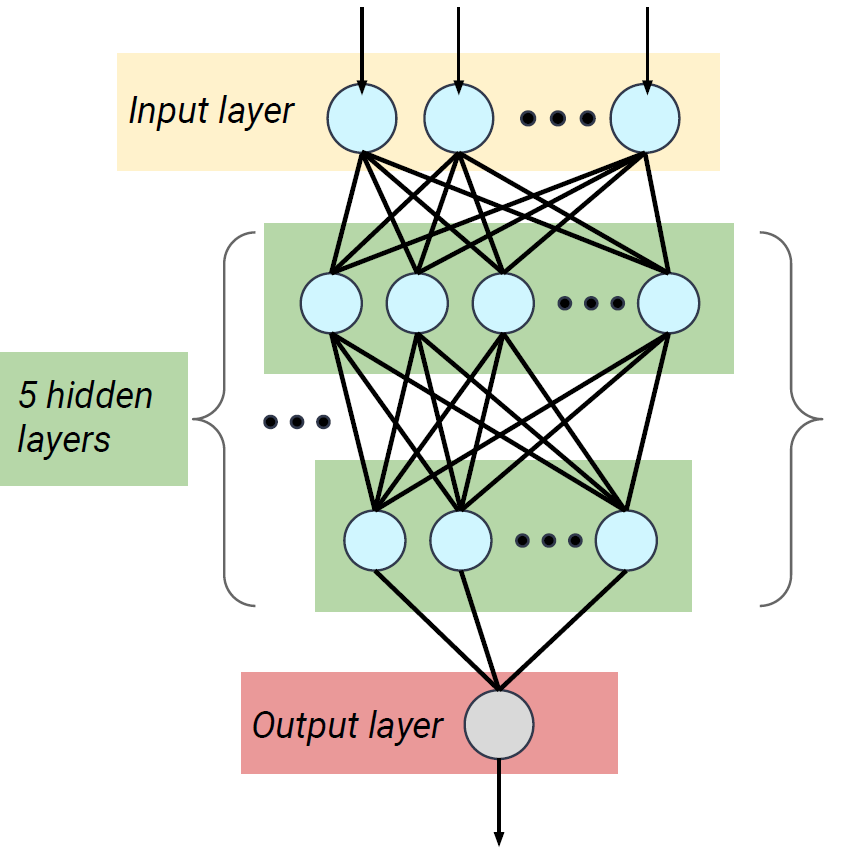
\includegraphics[width=0.55\textwidth]{figures/ml_dnn/DNNArchitecture.png}}
       \caption{Simplified DNN architecture visualisation.}
       \label{fig:DNNArchitecturePic}
\end{figure}

\begin{table}[ht]
    \centering
    \begin{tabular}{c|c|c|c}
     Layer(type) & Number of Neurons & Activation Functions & Regularizers\\
     \hline
     \hline
     Layer1(dense) & 64 & ReLu & L2\\
     Layer2(dense) & 32 & ReLu & L2\\
     Layer3(dense) & 32 & ReLu & L2\\
     Layer4(dense) & 32 & ReLu & L2\\
     Layer5(dense) & 16 & ReLu & L2\\
     Layer Out(dense) & 1 & Sigmoid & -\\
    \end{tabular}
    \caption{1-lepton DNN structure in merged and resolved signal regions.}
    \label{tab:1lepDNN layers}
\end{table}

%%%The importance of input features for the trained neural networks is quantified using the concept of SHAP (SHapley Additive exPlanations), 
%%%as introduced in the referenced NeurIPS paper \cite{LundbergLee2017}.
%%%%url = {https://proceedings.neurips.cc/paper/2017/file/8a20a8621978632d76c43dfd28b67767-Paper.pdf}
%%%SHAP aims to clarify the predictive output of the model for individual events by assessing the contribution of each input feature to the resulting decision (DNN score). For a complex model such as a neural network, an interpretable approximation can offer a simplified, more comprehensible explanation. This surrogate model mirrors the performance of the original model while being more accessible for interpretation.
%%%For the purpose of these calculations, we utilize one half of the MC samples from each signal region.

\section{Input Variables and Feature Engineering}
\label{input_variables}

We measure the impact of input features on our DNNs using SHAP (SHapley Additive exPlanations), as detailed by Lundberg and Lee in their NeurIPS paper \cite{LundbergLee2017}. SHAP helps understand how each feature influences the model's predictions (DNN scores) for individual events. It provides an interpretable approximation of complex neural networks, making the model's decisions easier to grasp. This approach creates a simplified model that still reflects the original's performance, but is more straightforward to interpret.

To optimize the DNN models, we use a backward feature elimination method guided by SHAP value rankings. This involves removing the least important input features step by step. After each round of elimination, the DNN models are retrained, and SHAP values are recalculated to update the feature rankings. In the end, we retain 15 input features for the merged category and 17 for the resolved category.
The final selection of input features for both categories is listed in Table~\ref{tab:1lepNN}, while their SHAP value rankings are shown in Figure~\ref{fig:1lepDNN_shap_rank}.
%%Figures \ref{fig:mer_inputs-part1} to \ref{fig:mer_inputs-part2} display the input feature distributions in the SRs. The differing shapes between signal and background in these figures demonstrate the effectiveness of the feature selection process.
The term ``full system'' refers to variables associated with the entire set of signal jet(s), lepton(s), and tagging jets.
The boson centrality, $\xi(V)$, is defined as :  
\begin{equation} \label{eq:centr} \xi(V)  = min(\Delta\eta_{-},\Delta\eta_{+}) \end{equation} where $$\Delta\eta_{-} = min(\eta_{\Vlep},\eta_{\Vhad}) - min(\etajo,\etajt)$$ and  $$\Delta\eta_{+} = max(\etajo,\etajt) - max(\eta_{\Vlep},\eta_{\Vhad}) $$
Figures~\ref{fig:mer_inputs-part1}, \ref{fig:mer_inputs-part2}, \ref{fig:res_inputs-part1}, and \ref{fig:res_inputs-part2} display the input feature distributions in the SRs. The differing shapes between signal and background in these figures demonstrate the effectiveness of the feature selection process.

Figure~\ref{fig:ROCChecks} shows a comparison between the performance of the initial and final DNN models in both the merged and resolved categories, indicating they are similarly effective. To understand this comparison, we define signal efficiency and background rejection as follows:

\begin{equation}
\text{Signal Efficiency} = \frac{\text{Number of Signal events with DNN} > X}{\text{Total Number of Signal events}}
\end{equation}

\begin{equation}
\text{Background Rejection} = \frac{\text{Number of Background events with DNN} < X}{\text{Total Number of Background events}}.
\end{equation}

%These definitions help in evaluating the DNN's ability to correctly identify signal events and reject background events.

\begin{figure}[ht]
      \centering
       \subfloat[\emph{ROC Curve}]{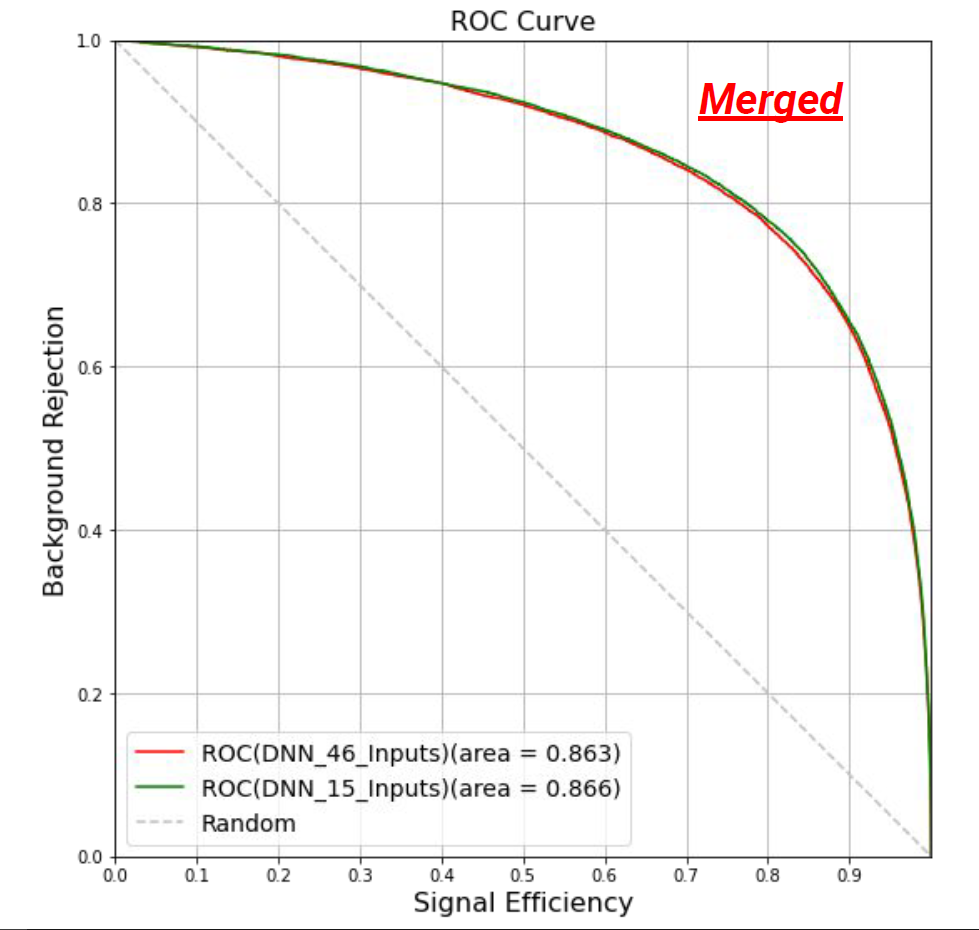
\includegraphics[width=0.4\textwidth]{figures/ml_dnn/ROCImpactMerged.png}}
       \subfloat[\emph{ROC Curve}]{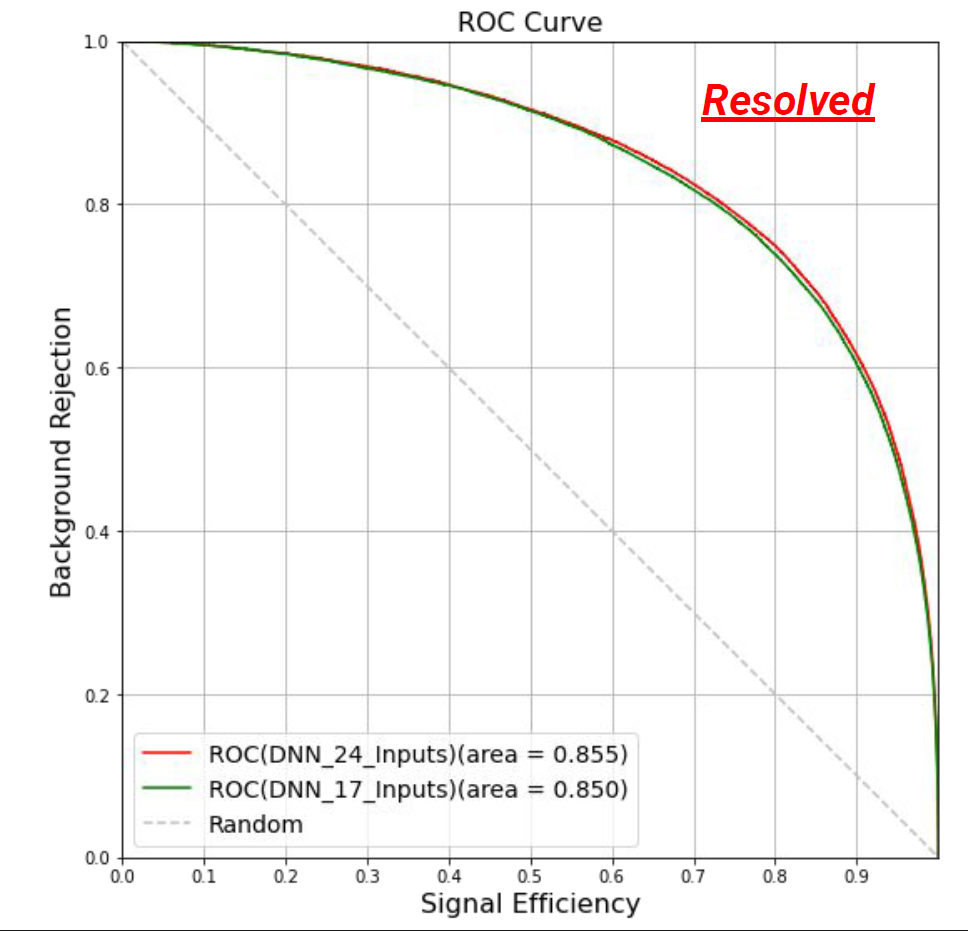
\includegraphics[width=0.4\textwidth]{figures/ml_dnn/ROCImpactRes.png}}
       \caption{ROC curves for the DNN models in the merged (a) and resolved (b) categories. Here, ``area'' refers to the AUC (Area Under the ROC Curve). The AUC values are computed to offer quantitative measures of performance.}
       \label{fig:ROCChecks}
\end{figure}

%%While further refinement of this input feature roster is conceivable through continued iteration, the marginal gains may be limited, given that uncertainties have not been factored into the selection process.

\begin{table}[ht]
    \centering
    \begin{tabular}{r|c|c}
     feature & merged & resolved\\
     \hline
     \hline
     signal jet(s) mass & $m(J^\text{sig})$ & $m(jj^\text{sig})$\\
     signal jet transverse momentum & $ - $ & $p_\text{T}(j^\text{sig}_\text{lead})$ and  $p_\text{T}(j^\text{sig}_\text{sublead})$\\
     signal jet width & $ - $ & $W(j^\text{sig}_\text{lead})$ and  $W(j^\text{sig}_\text{sublead})$\\
     dijet(signal jet) transverse momentum & $ - $ & $p_\text{T}(jj^\text{sig})$\\
     number of tracks associated to the signal jet(s) & $N_\text{trk}(J^\text{sig})$ & -\\
     multiplicity of B-tagged jets & $N(j^\text{B-tagged})$ & -\\
     multiplicity of forward jets & $N(j^\text{forward})$ & -\\
     multiplicity of track jets & - & $N(j^\text{track})$\\
     diboson mass & $m(V^\text{had}V^\text{lep})$ & $ - $\\
     leading tagging jet mass & $m(j^\text{tag}_\text{lead})$ & $ - $\\
     full system mass & $ - $ & $m(V^\text{had}V^\text{lep}+jj^\text{tag})$\\
     tagging jet transverse momentum & $p_\text{T}(j^\text{tag}_\text{sublead})$ & $p_\text{T}(j^\text{tag}_\text{lead})$ and $p_\text{T}(j^\text{tag}_\text{sublead})$\\
     tagging jet width & $W(j^\text{tag}_\text{lead})$ and $W(j^\text{tag}_\text{sublead})$  & $ - $\\
     boson centrality & $\xi(V)$ & $ - $\\
     pseudo-rapidity of tagging jets & - & $\eta(j^\text{tag}_\text{lead})$ and $ \eta(j^\text{tag}_\text{sublead})$\\
     pseudo-rapidity of lepton & - & $\eta(l)$\\
     lepton transverse momentum & $p_\text{T}(l)$ & -\\
%%%     jets multiplicity & \multicolumn{2}{c}{$N(j)$}\\
     number of tracks associated to the tagging jets & $N_\text{trk}(j^\text{tag}_\text{lead})$ and $N_\text{trk}(j^\text{tag}_\text{sublead})$ & -\\
     jets multiplicity & \multicolumn{2}{c}{$N(j)$}\\
     tagging jets mass & \multicolumn{2}{c}{$m(jj^\text{tag})$}\\
     tagging jet separation & \multicolumn{2}{c}{$\Delta\eta(j^\text{tag}_\text{lead},j^\text{tag}_\text{sublead})$}\\
     lepton energy & \multicolumn{2}{c}{$E_{\ell}$}\\
    \end{tabular}
    \caption{Input variables for the 1-lepton DNN in merged and resolved signal regions.}
    \label{tab:1lepNN}
\end{table}

\begin{figure}[ht]
      \centering
       \subfloat[\emph{Rankings Merged}]{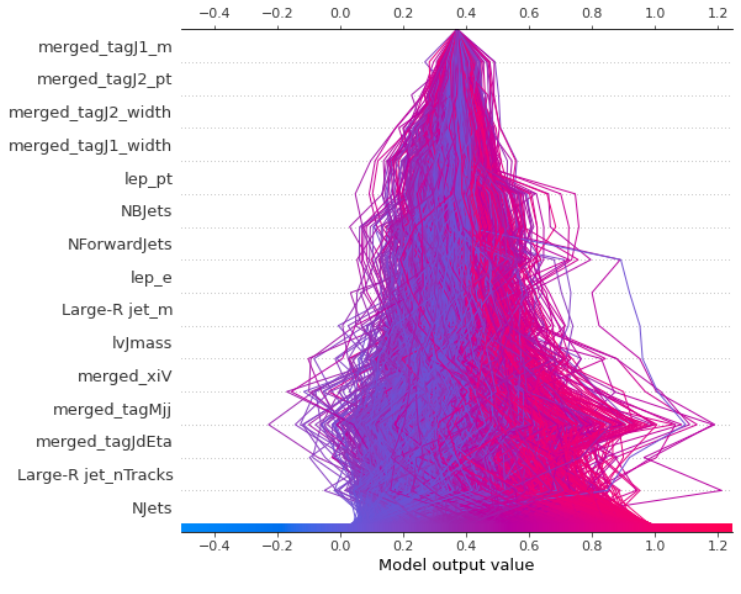
\includegraphics[width=0.4\textwidth]{figures/ml_dnn/rankings/decision_plot_mer.PNG}}
       \hspace{5mm}
       \subfloat[\emph{Rankings Resolved}]{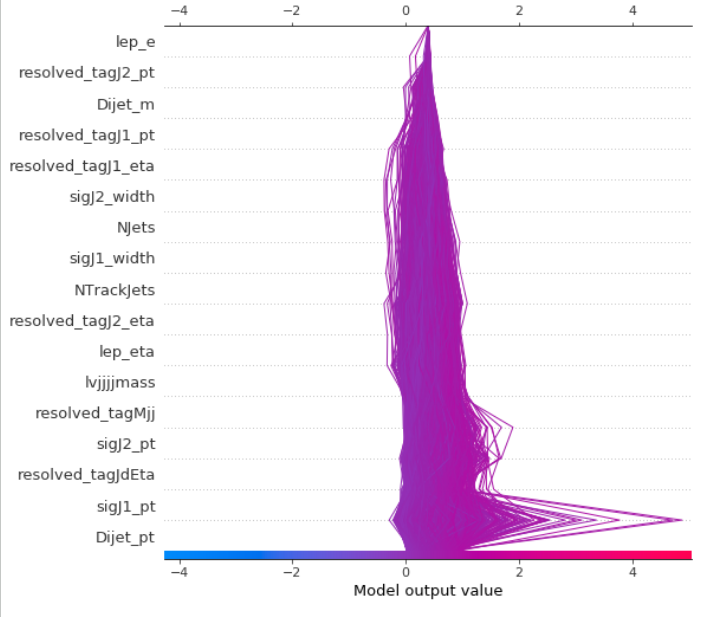
\includegraphics[width=0.4\textwidth]{figures/ml_dnn/rankings/decision_plot_res.PNG}}
       \caption{SHAP value rankings of input variables for both merged and resolved regimes; variables with lower impact appear at the top.}
       \label{fig:1lepDNN_shap_rank}
\end{figure}

\begin{figure}[ht]
 \centering
  % Row 1
  \subfloat[]{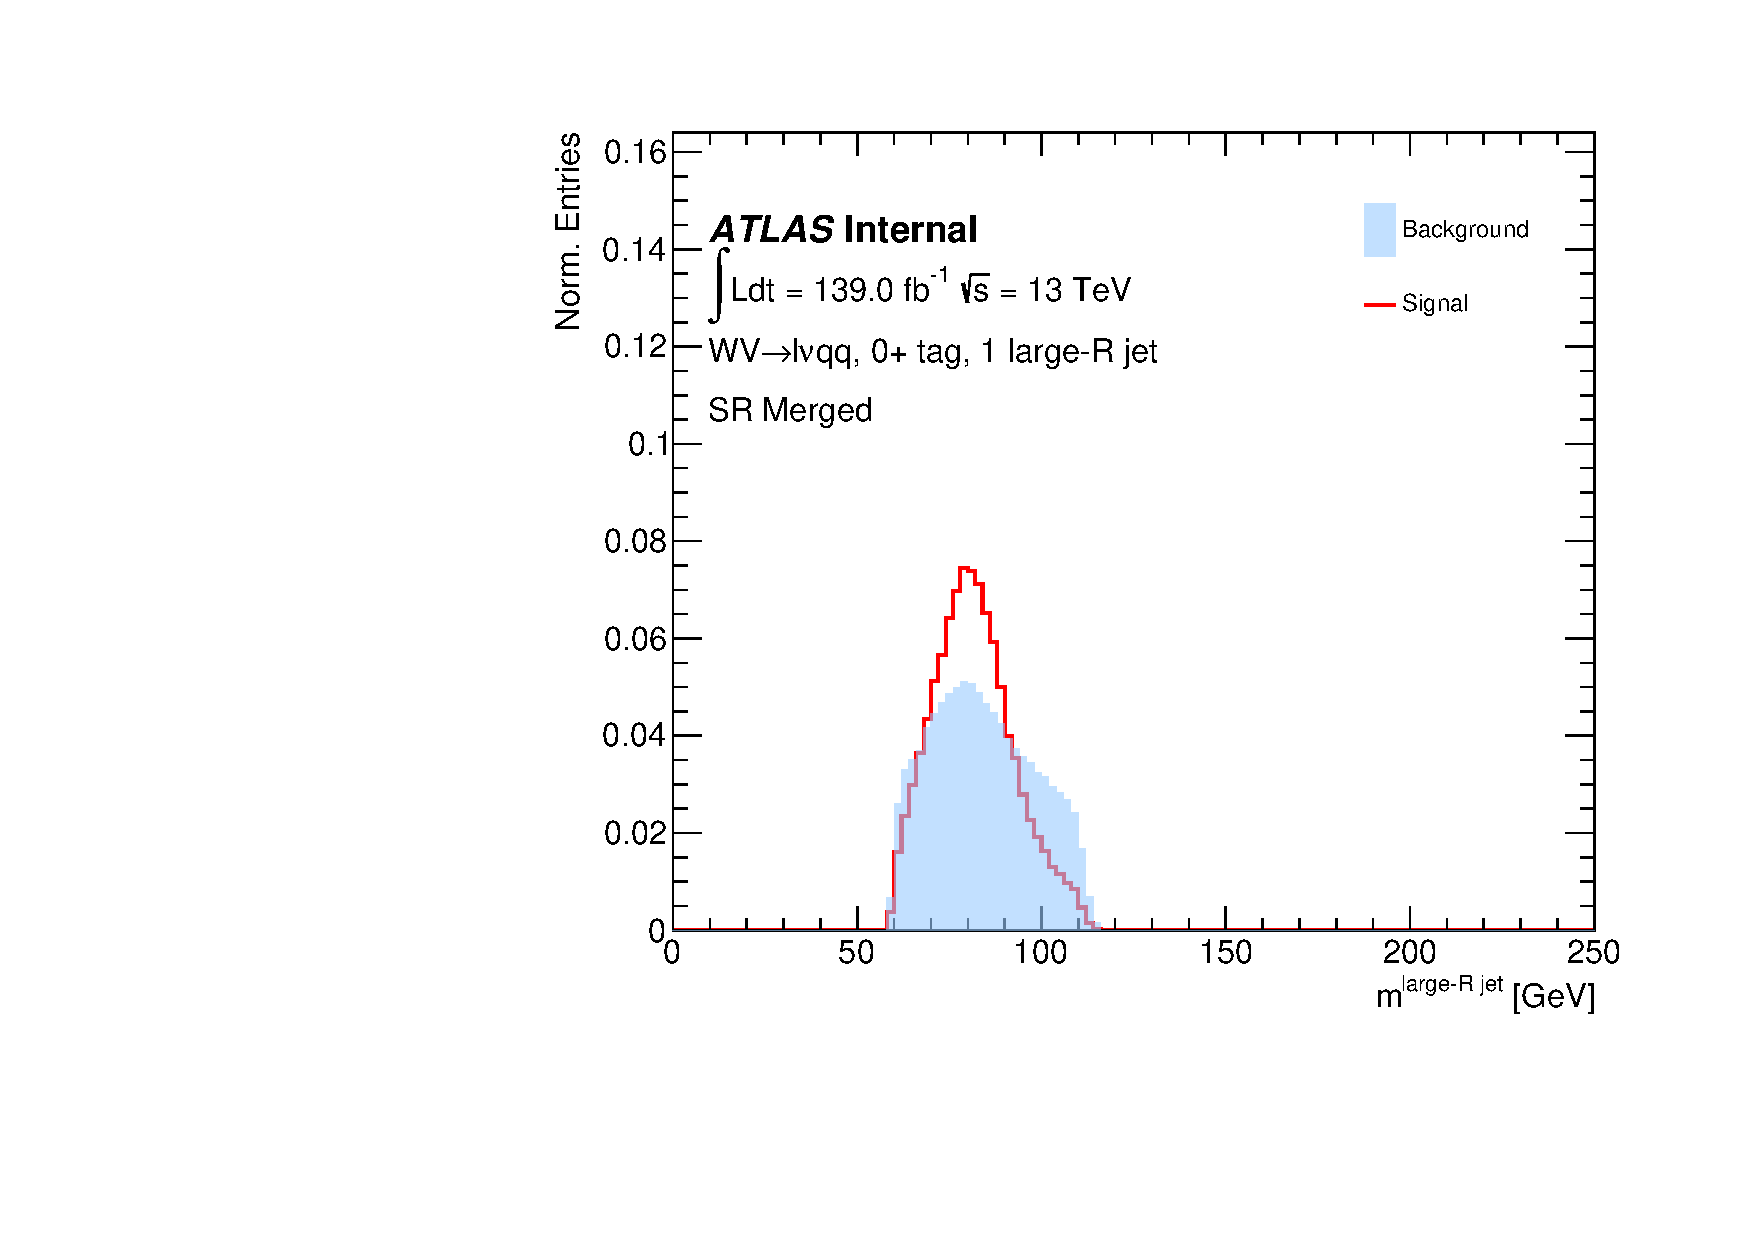
\includegraphics[width=0.3\textwidth]{figures/ml_dnn/variables/SR_Mer/norm_plot_fatJ_m.pdf}}\quad
  \subfloat[]{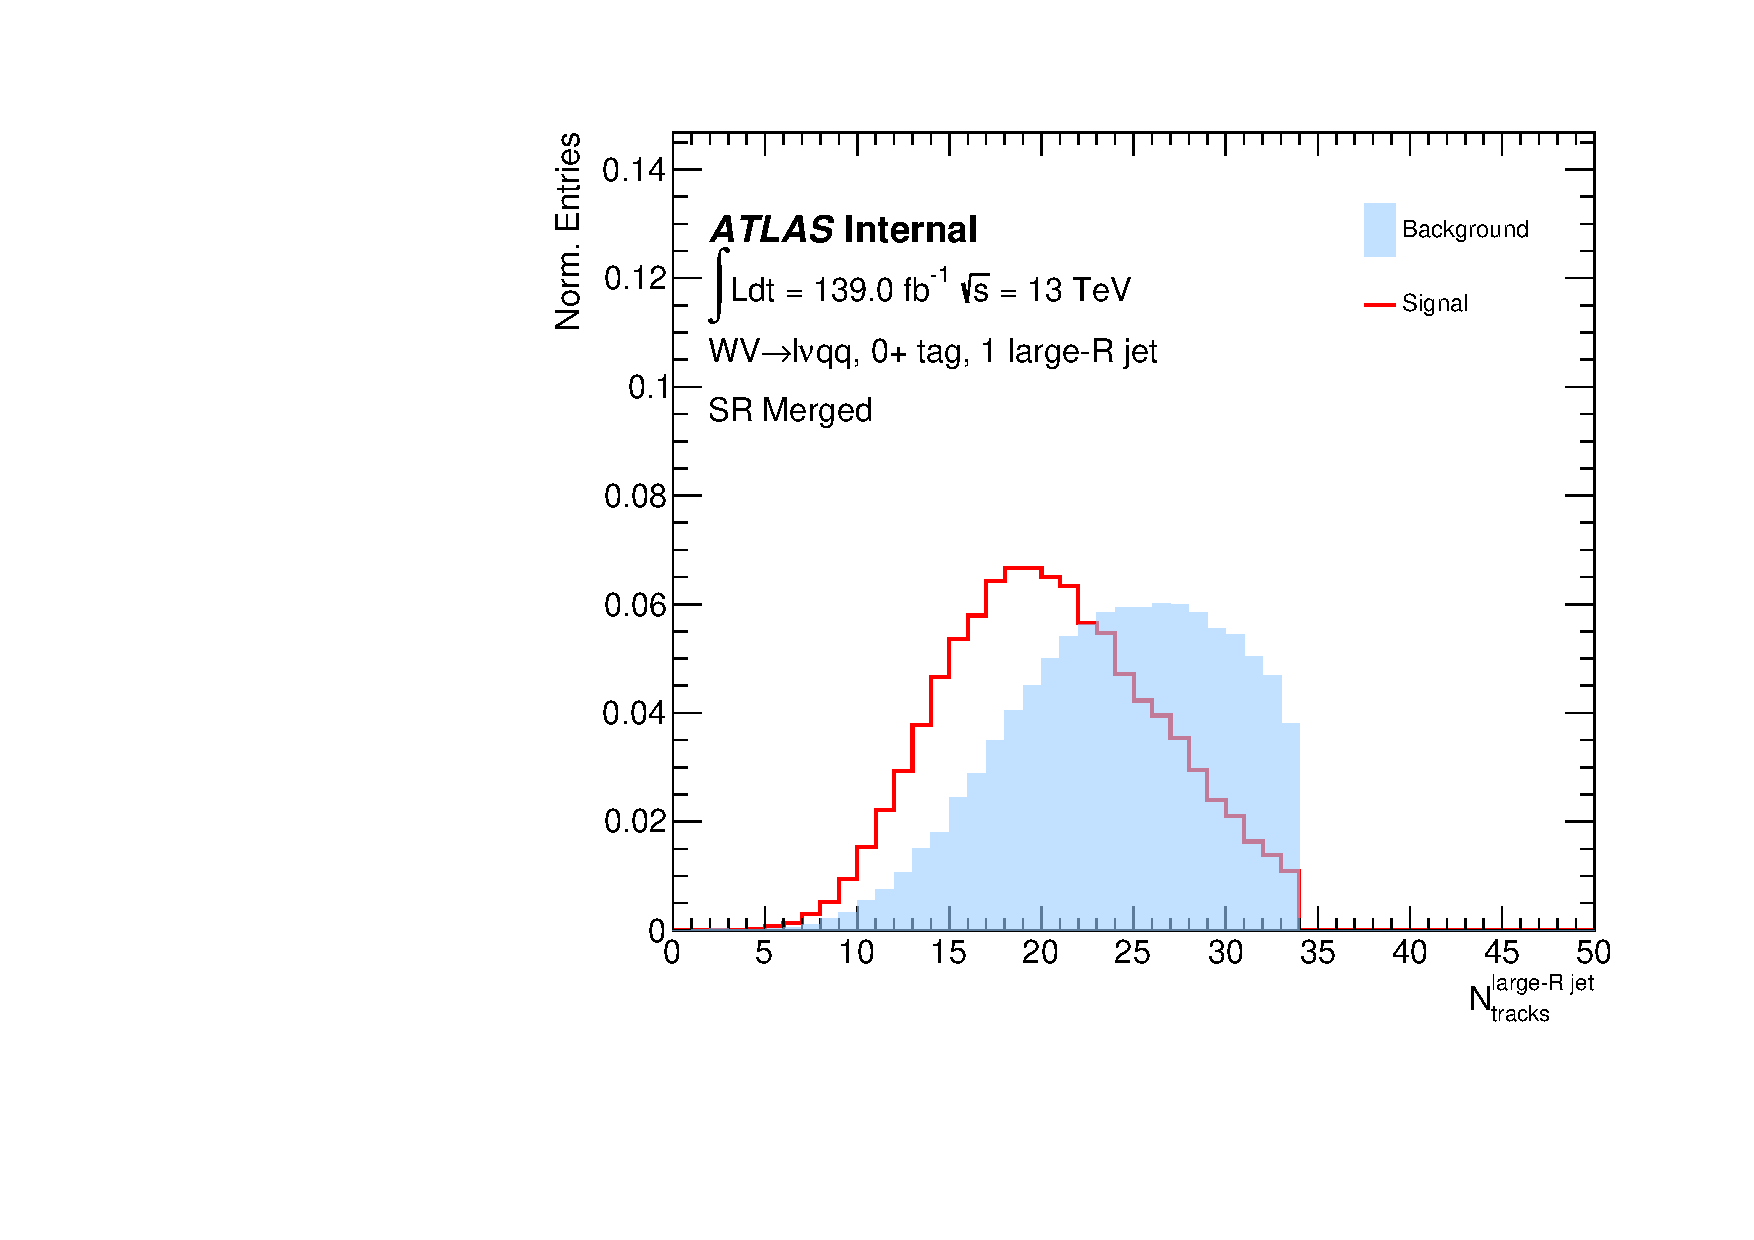
\includegraphics[width=0.3\textwidth]{figures/ml_dnn/variables/SR_Mer/norm_plot_fatJ_nTracks.pdf}}\quad
  \subfloat[]{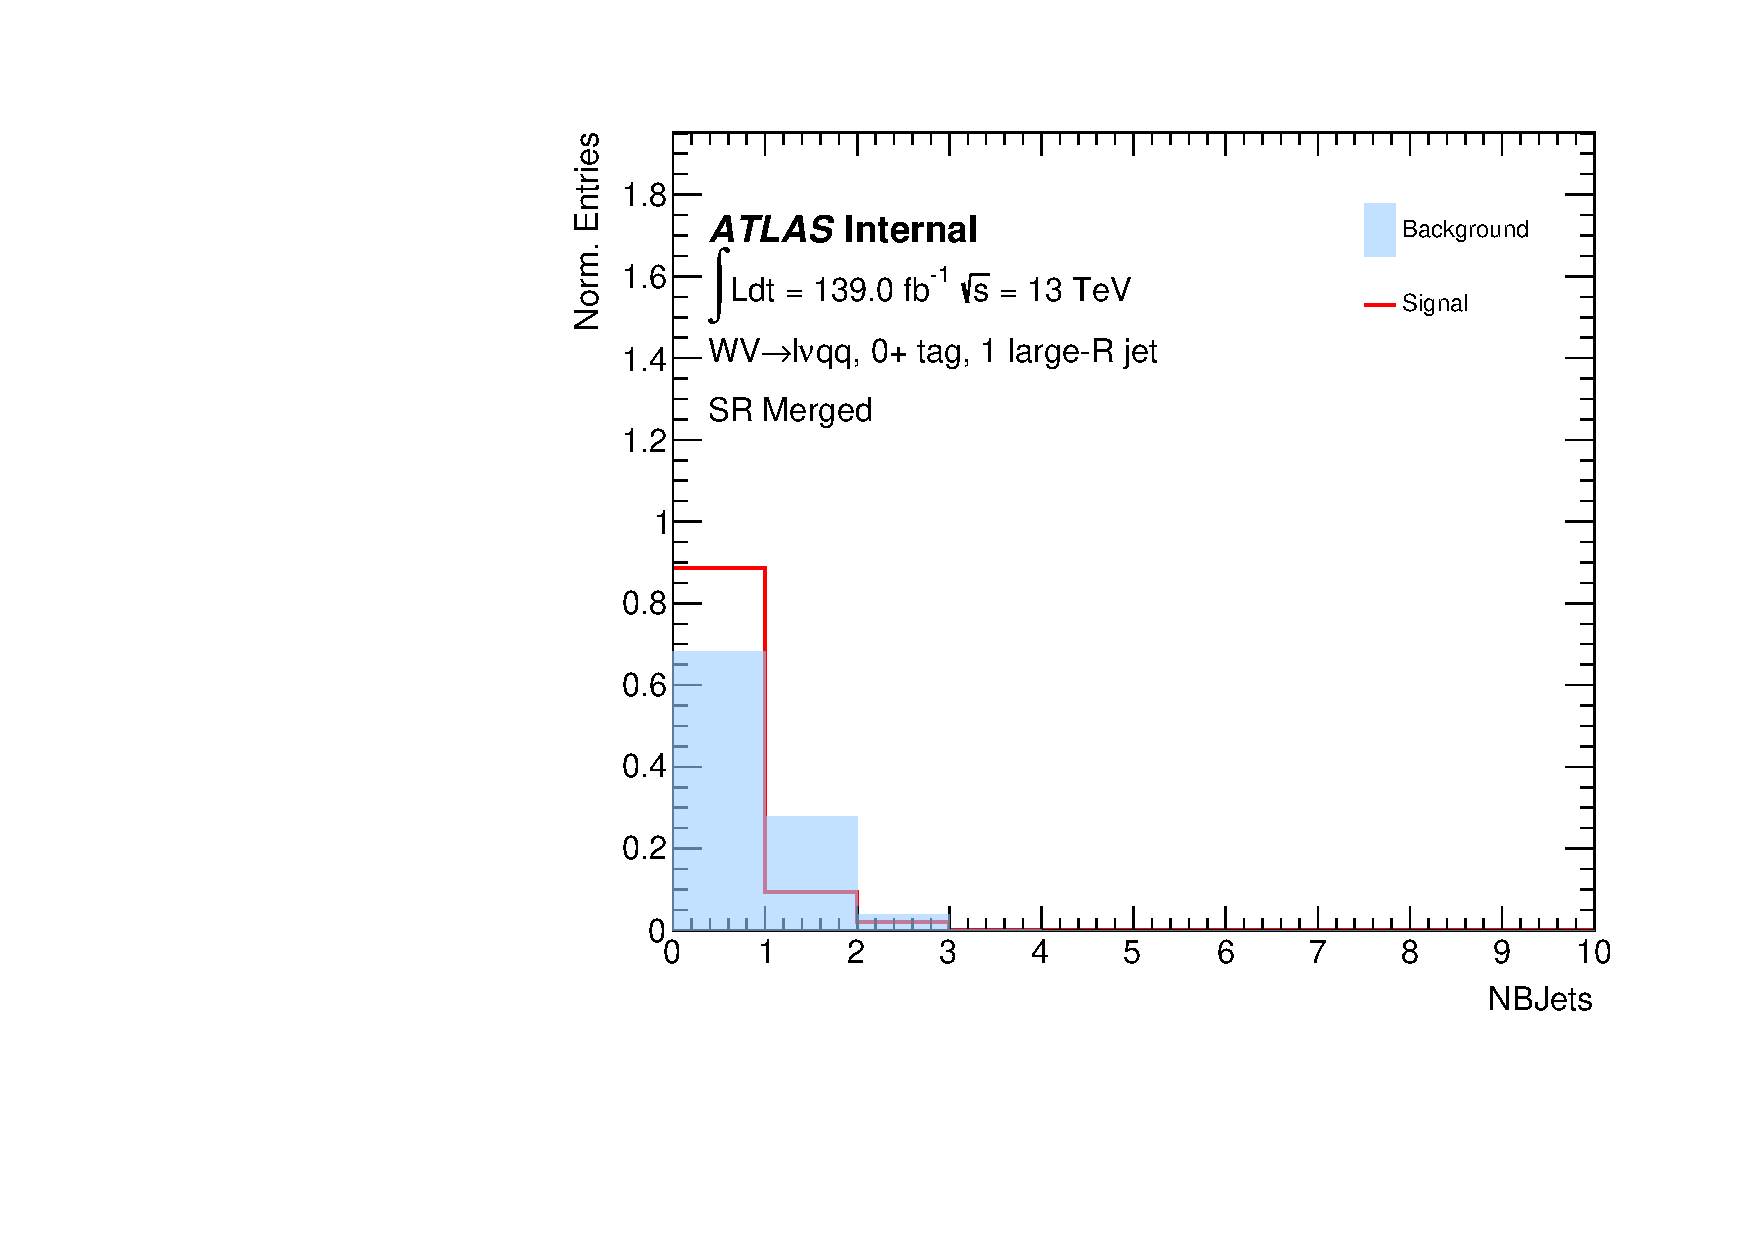
\includegraphics[width=0.3\textwidth]{figures/ml_dnn/variables/SR_Mer/norm_plot_NBJets.pdf}}

  % Row 2
  \subfloat[]{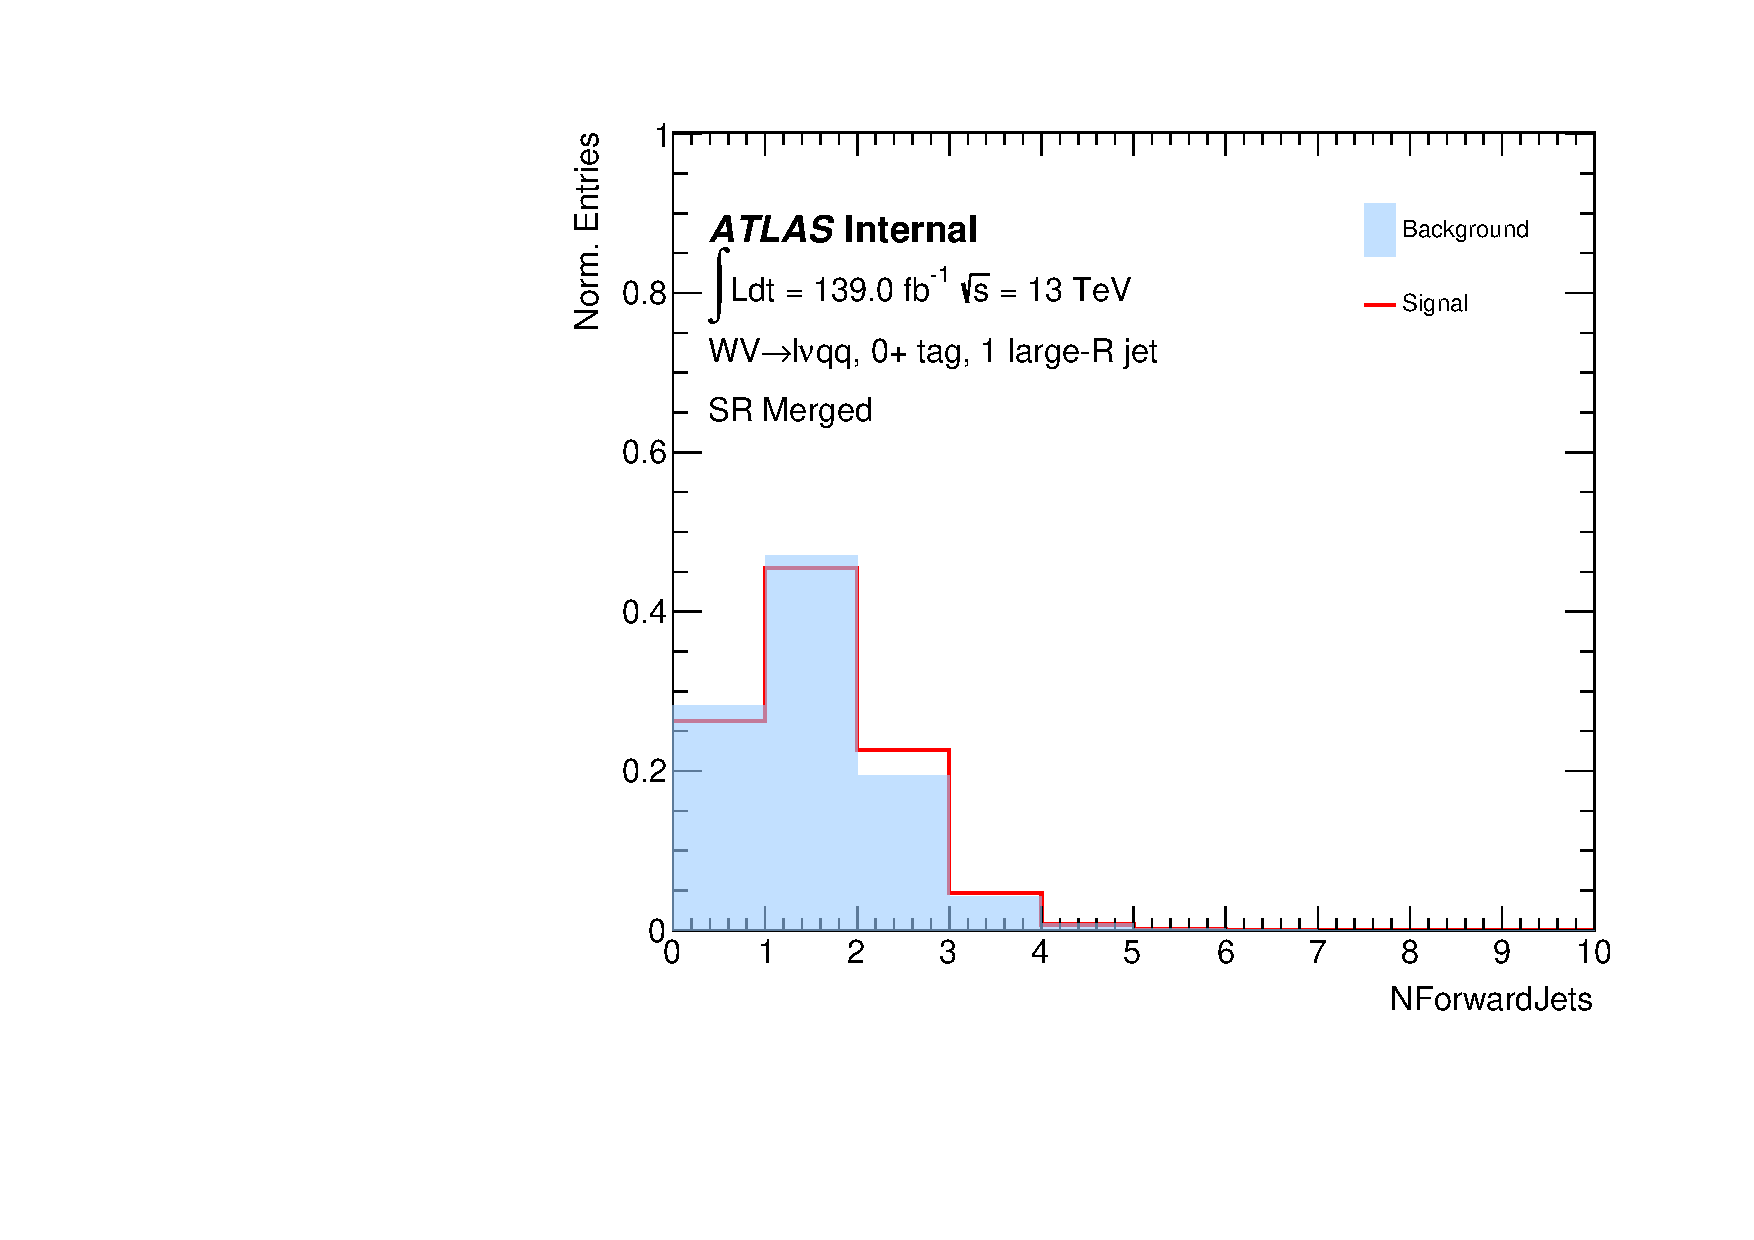
\includegraphics[width=0.3\textwidth]{figures/ml_dnn/variables/SR_Mer/norm_plot_NForwardJets.pdf}}\quad
  \subfloat[]{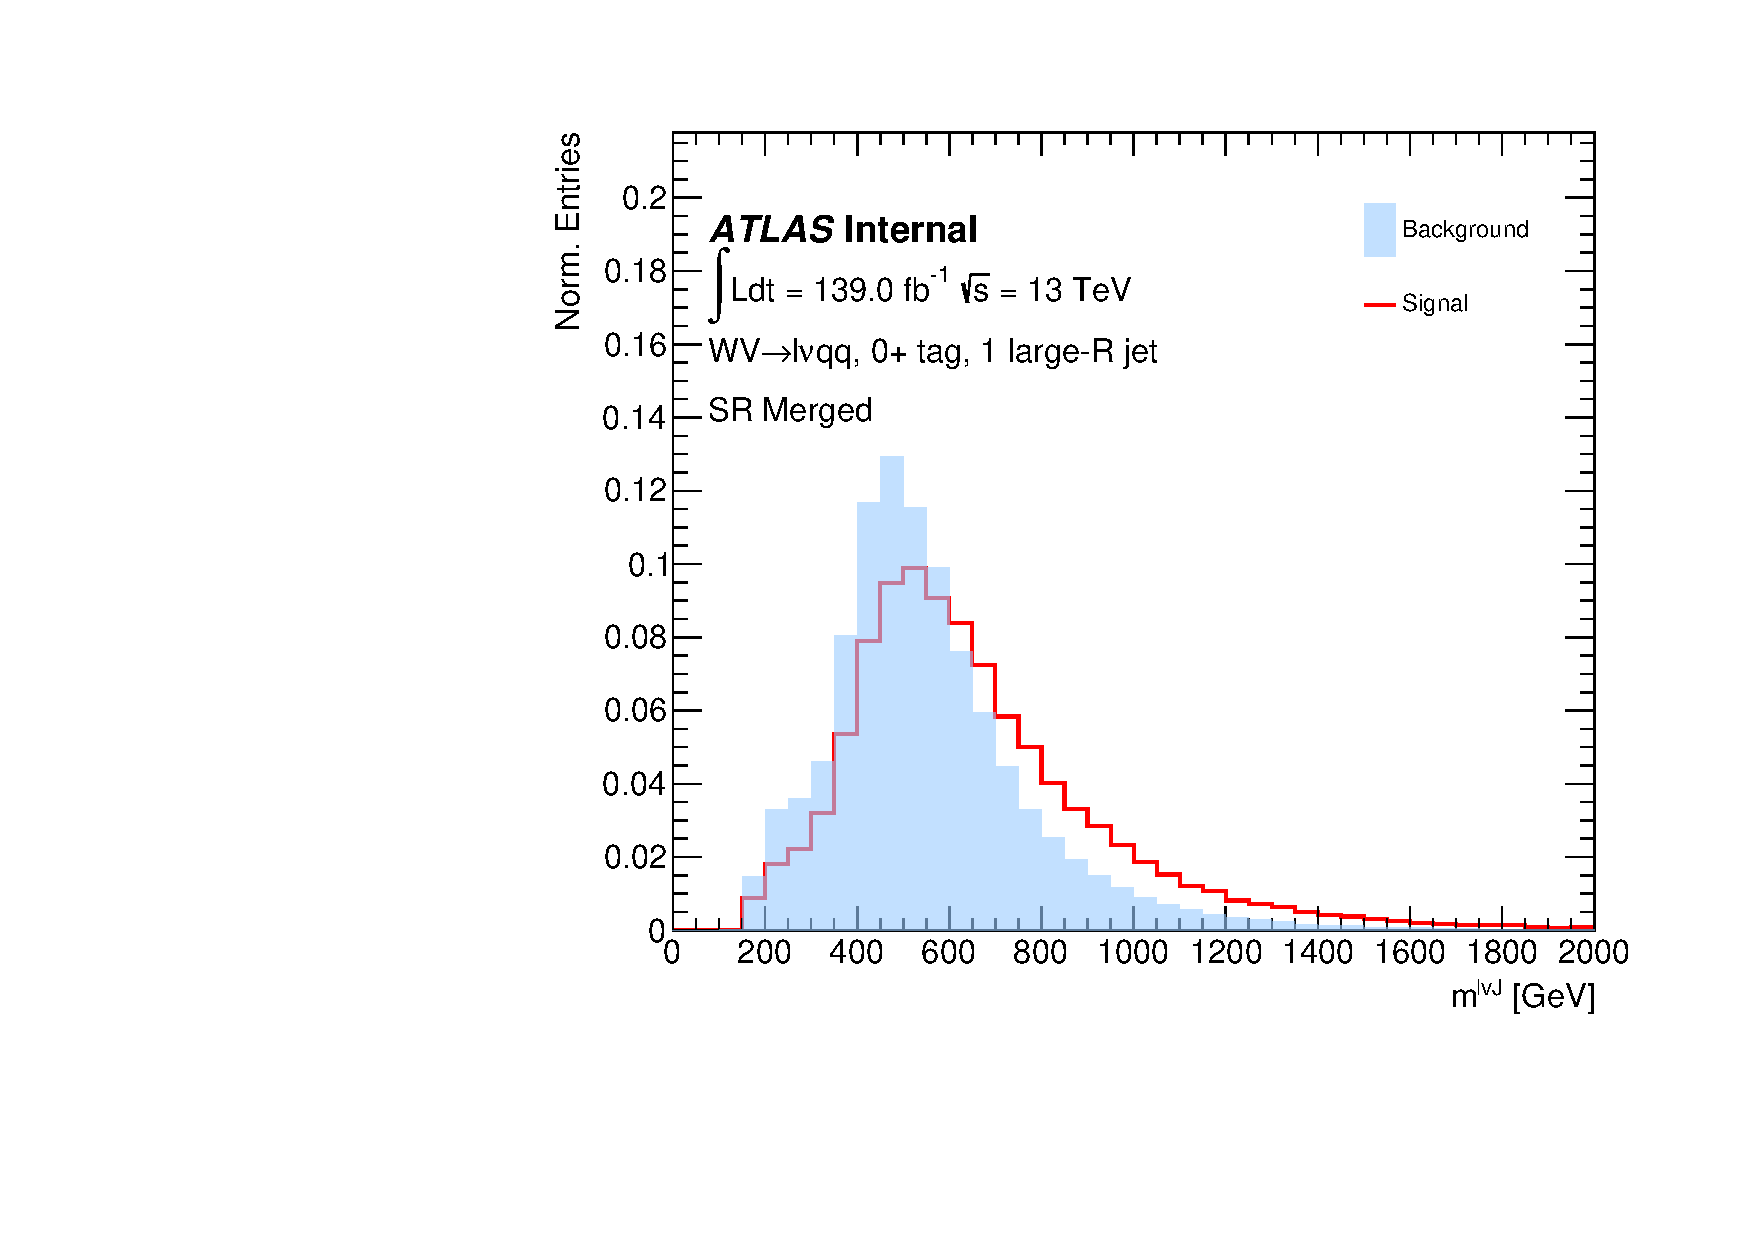
\includegraphics[width=0.3\textwidth]{figures/ml_dnn/variables/SR_Mer/norm_plot_lvJmass.pdf}}\quad
  \subfloat[]{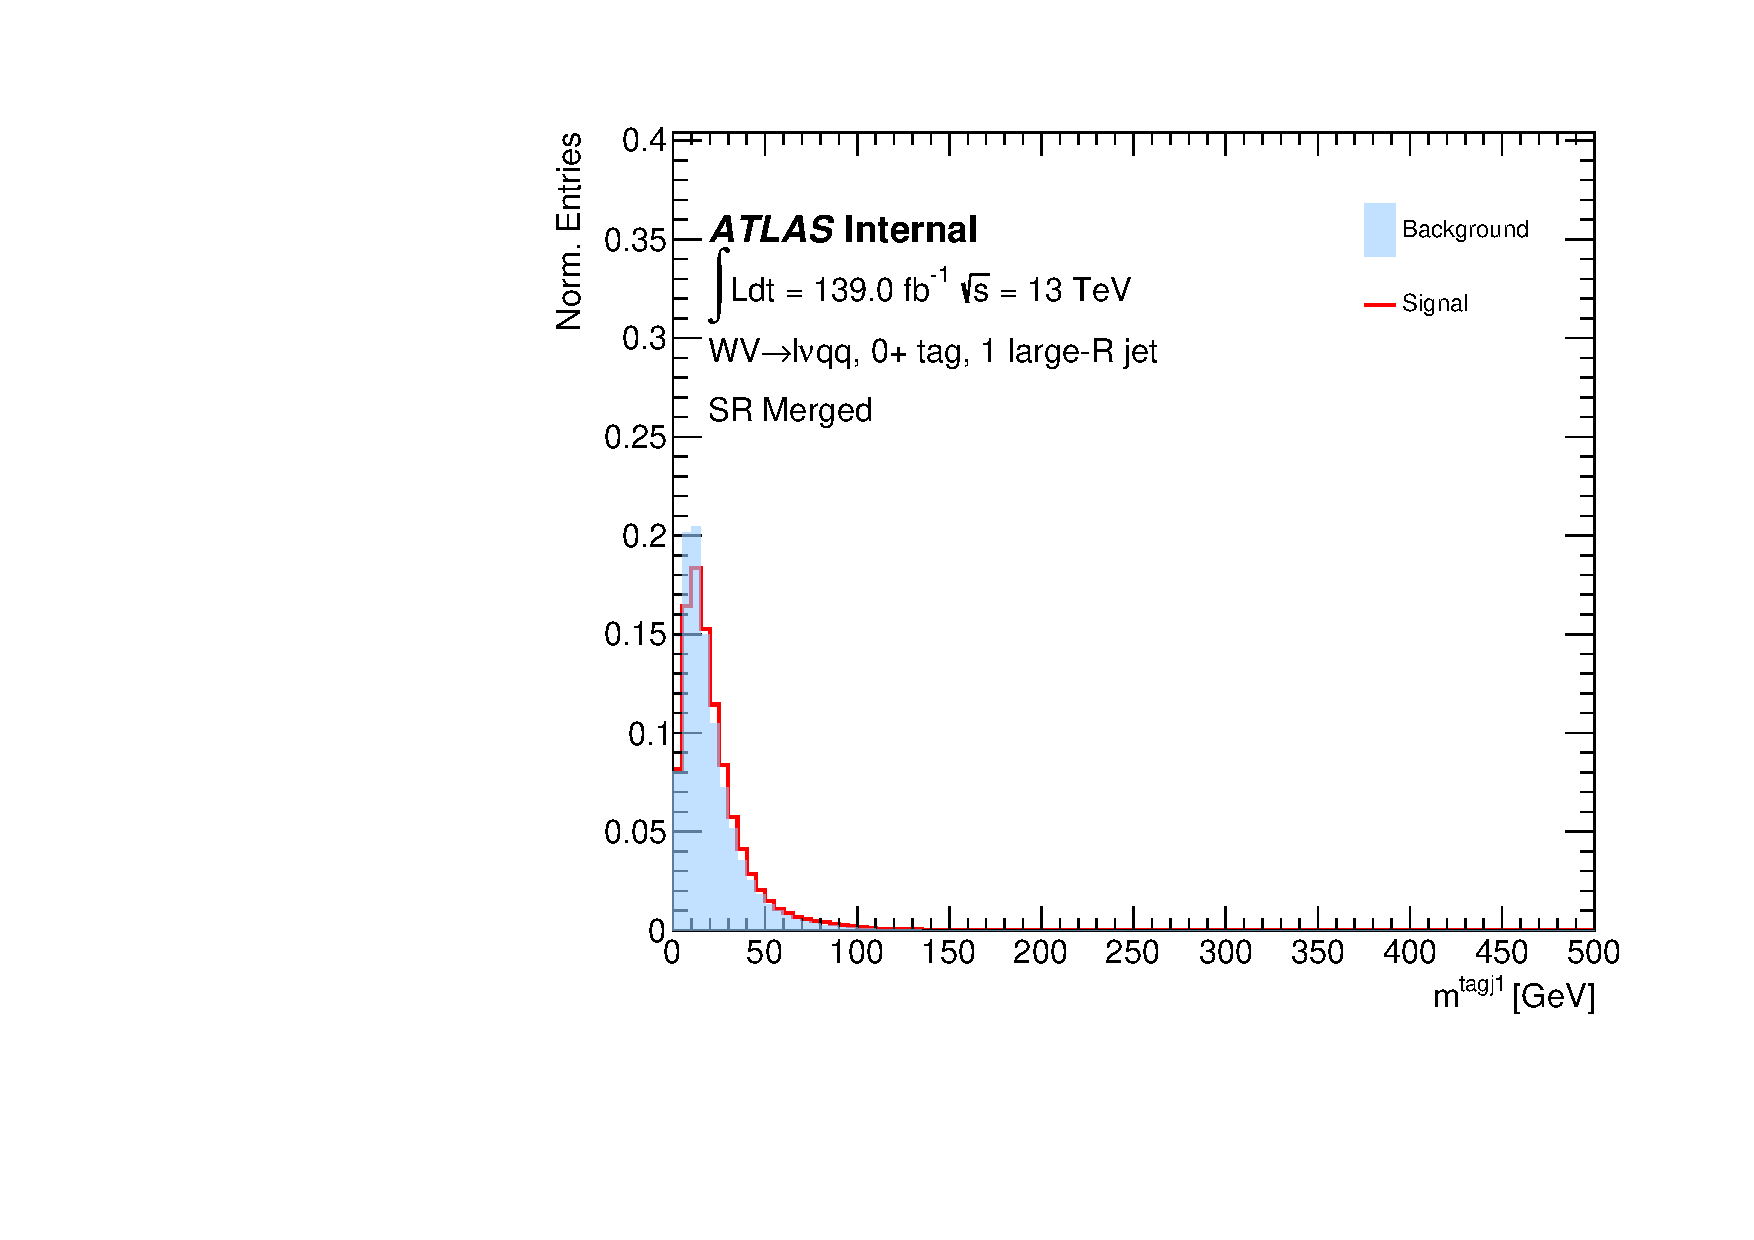
\includegraphics[width=0.3\textwidth]{figures/ml_dnn/variables/SR_Mer/norm_plot_merged_tagJ1_m.pdf}}

  % Row 3
%%  \subfloat[]{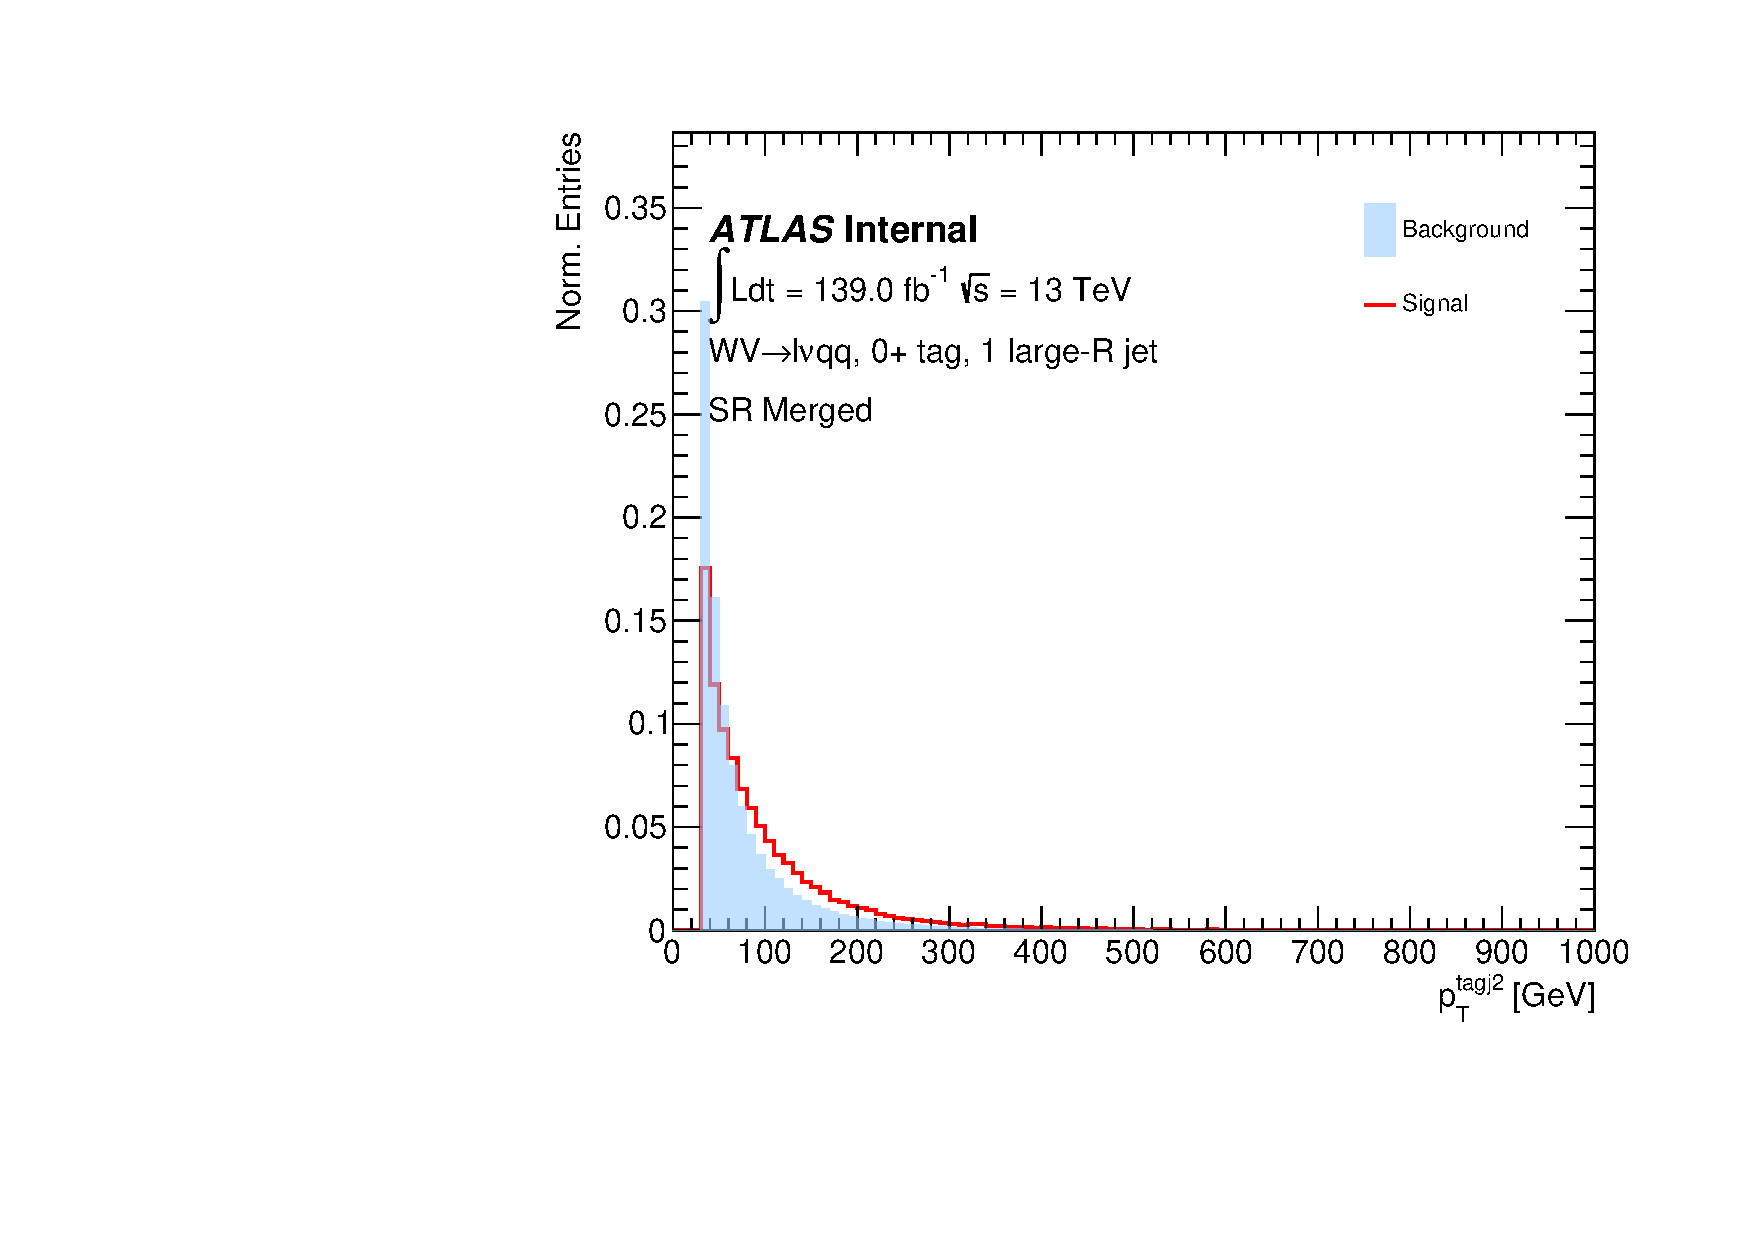
\includegraphics[width=0.3\textwidth]{figures/ml_dnn/variables/SR_Mer/norm_plot_merged_tagJ2_pt.pdf}}\quad
%%  \subfloat[]{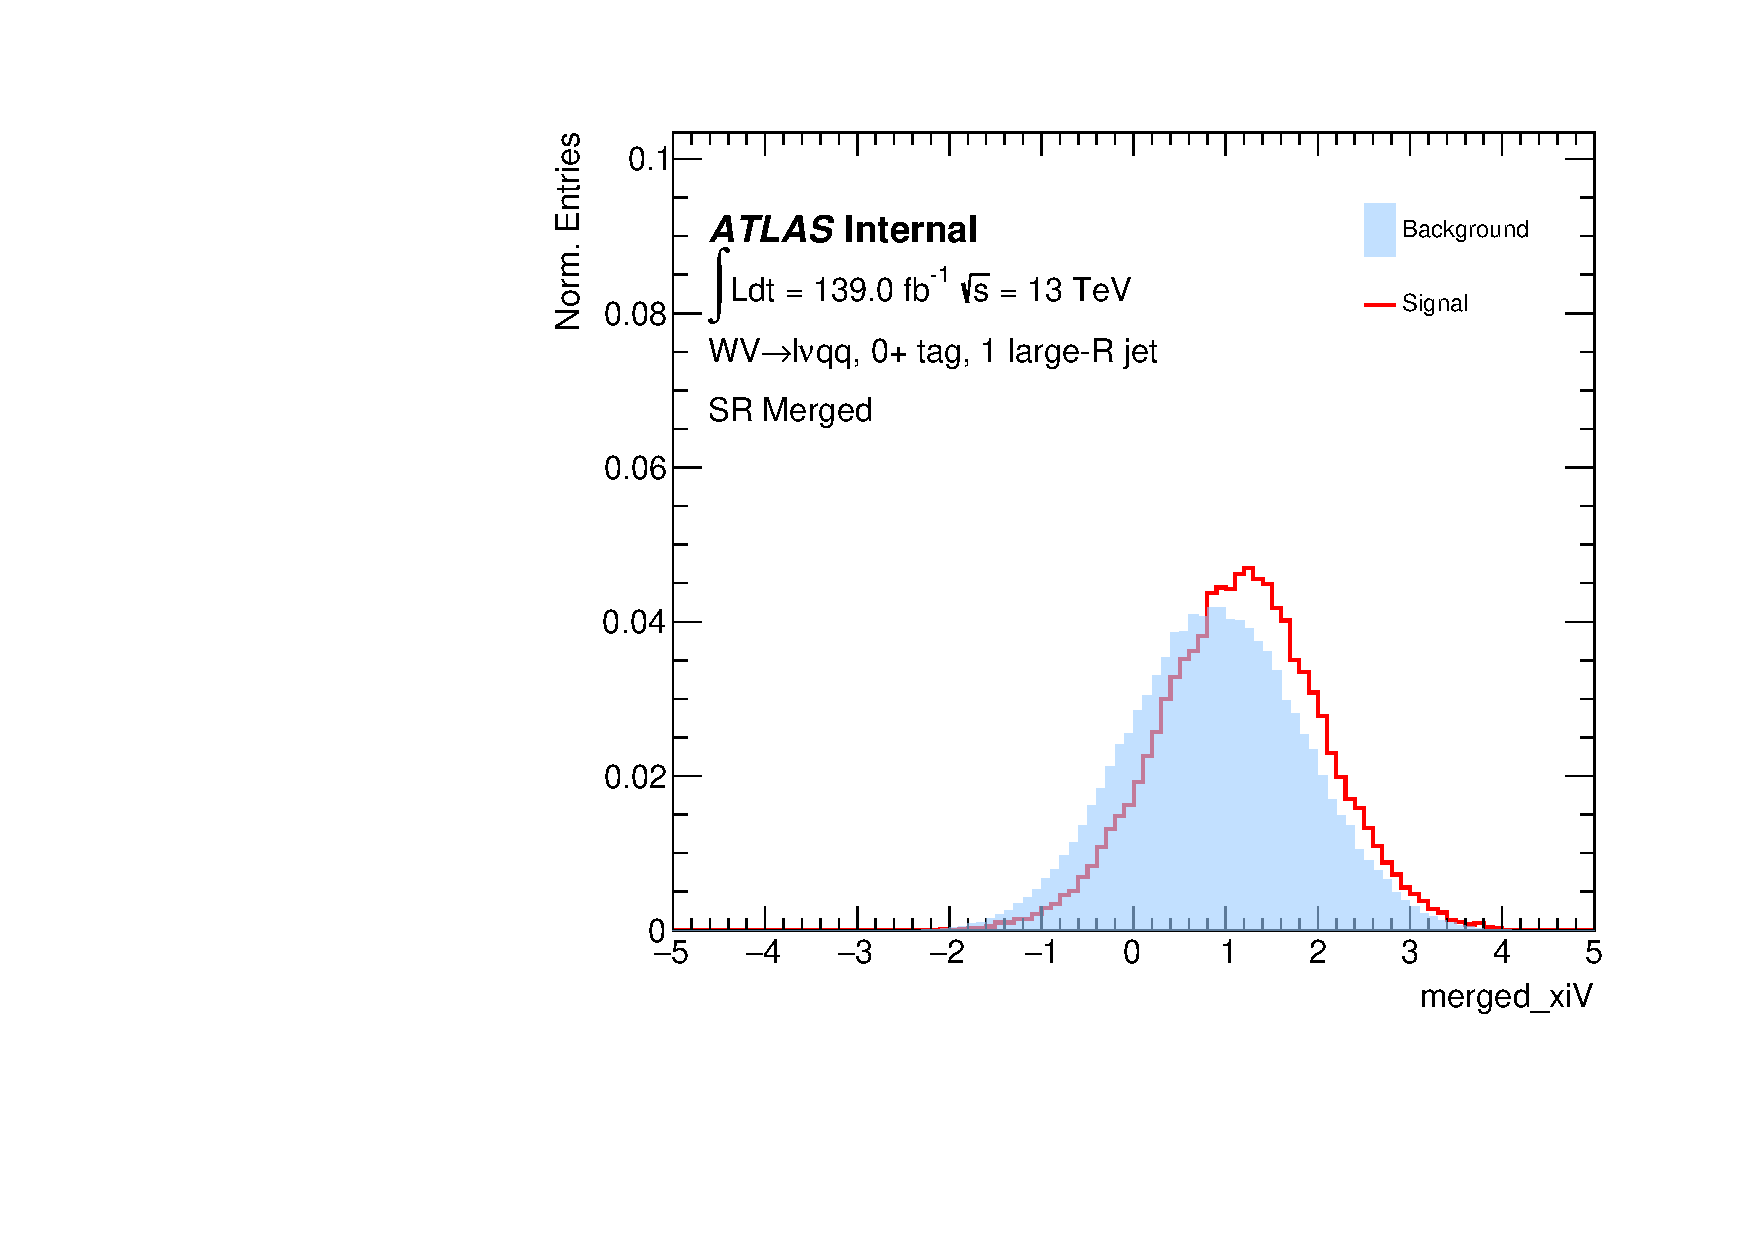
\includegraphics[width=0.3\textwidth]{figures/ml_dnn/variables/SR_Mer/norm_plot_merged_xiV.pdf}}\quad
%%  \subfloat[]{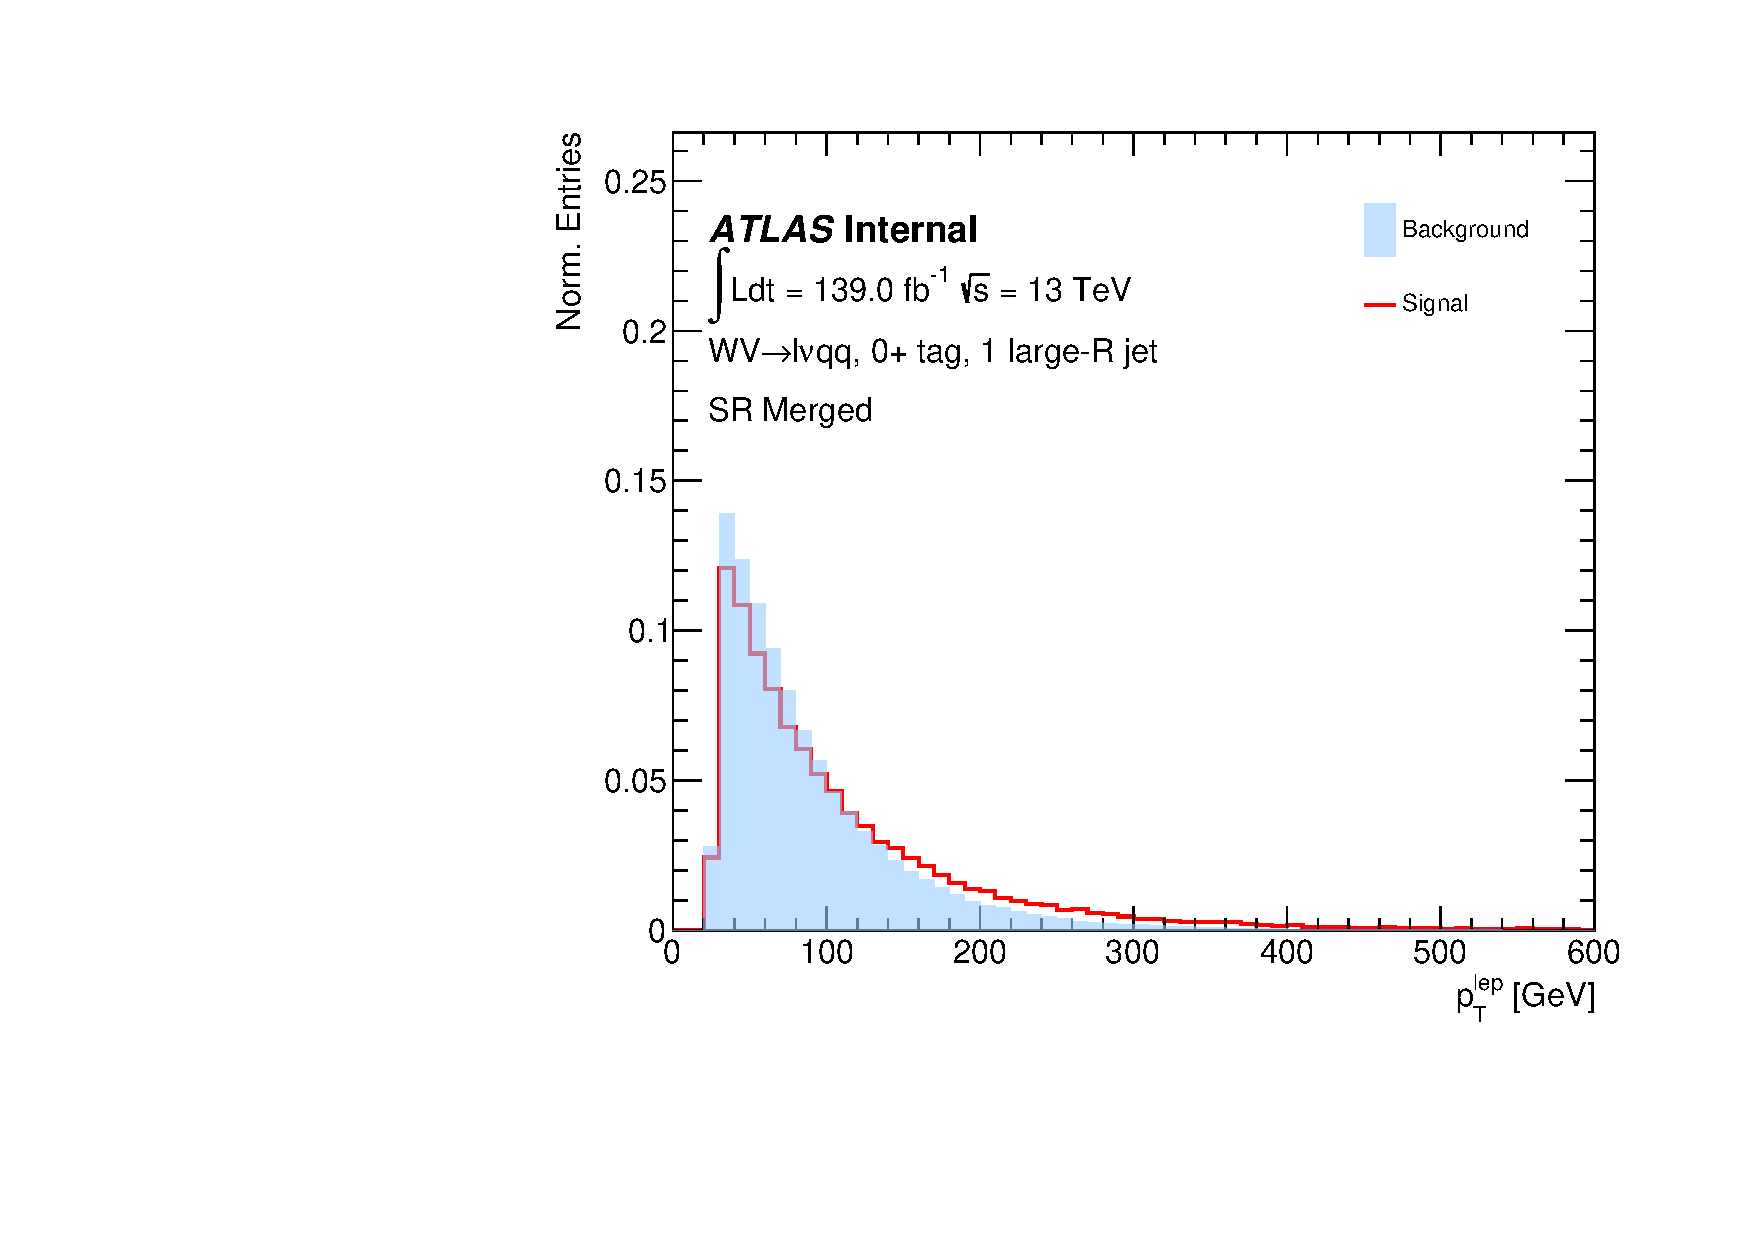
\includegraphics[width=0.3\textwidth]{figures/ml_dnn/variables/SR_Mer/norm_plot_lep_pt.pdf}}

 \caption{Distributions of input variables in the Merged SR (Continued on next page)}
 \label{fig:mer_inputs-part1}
\end{figure}

\begin{figure}[ht]
 \centering
  % Row 3
  \subfloat[]{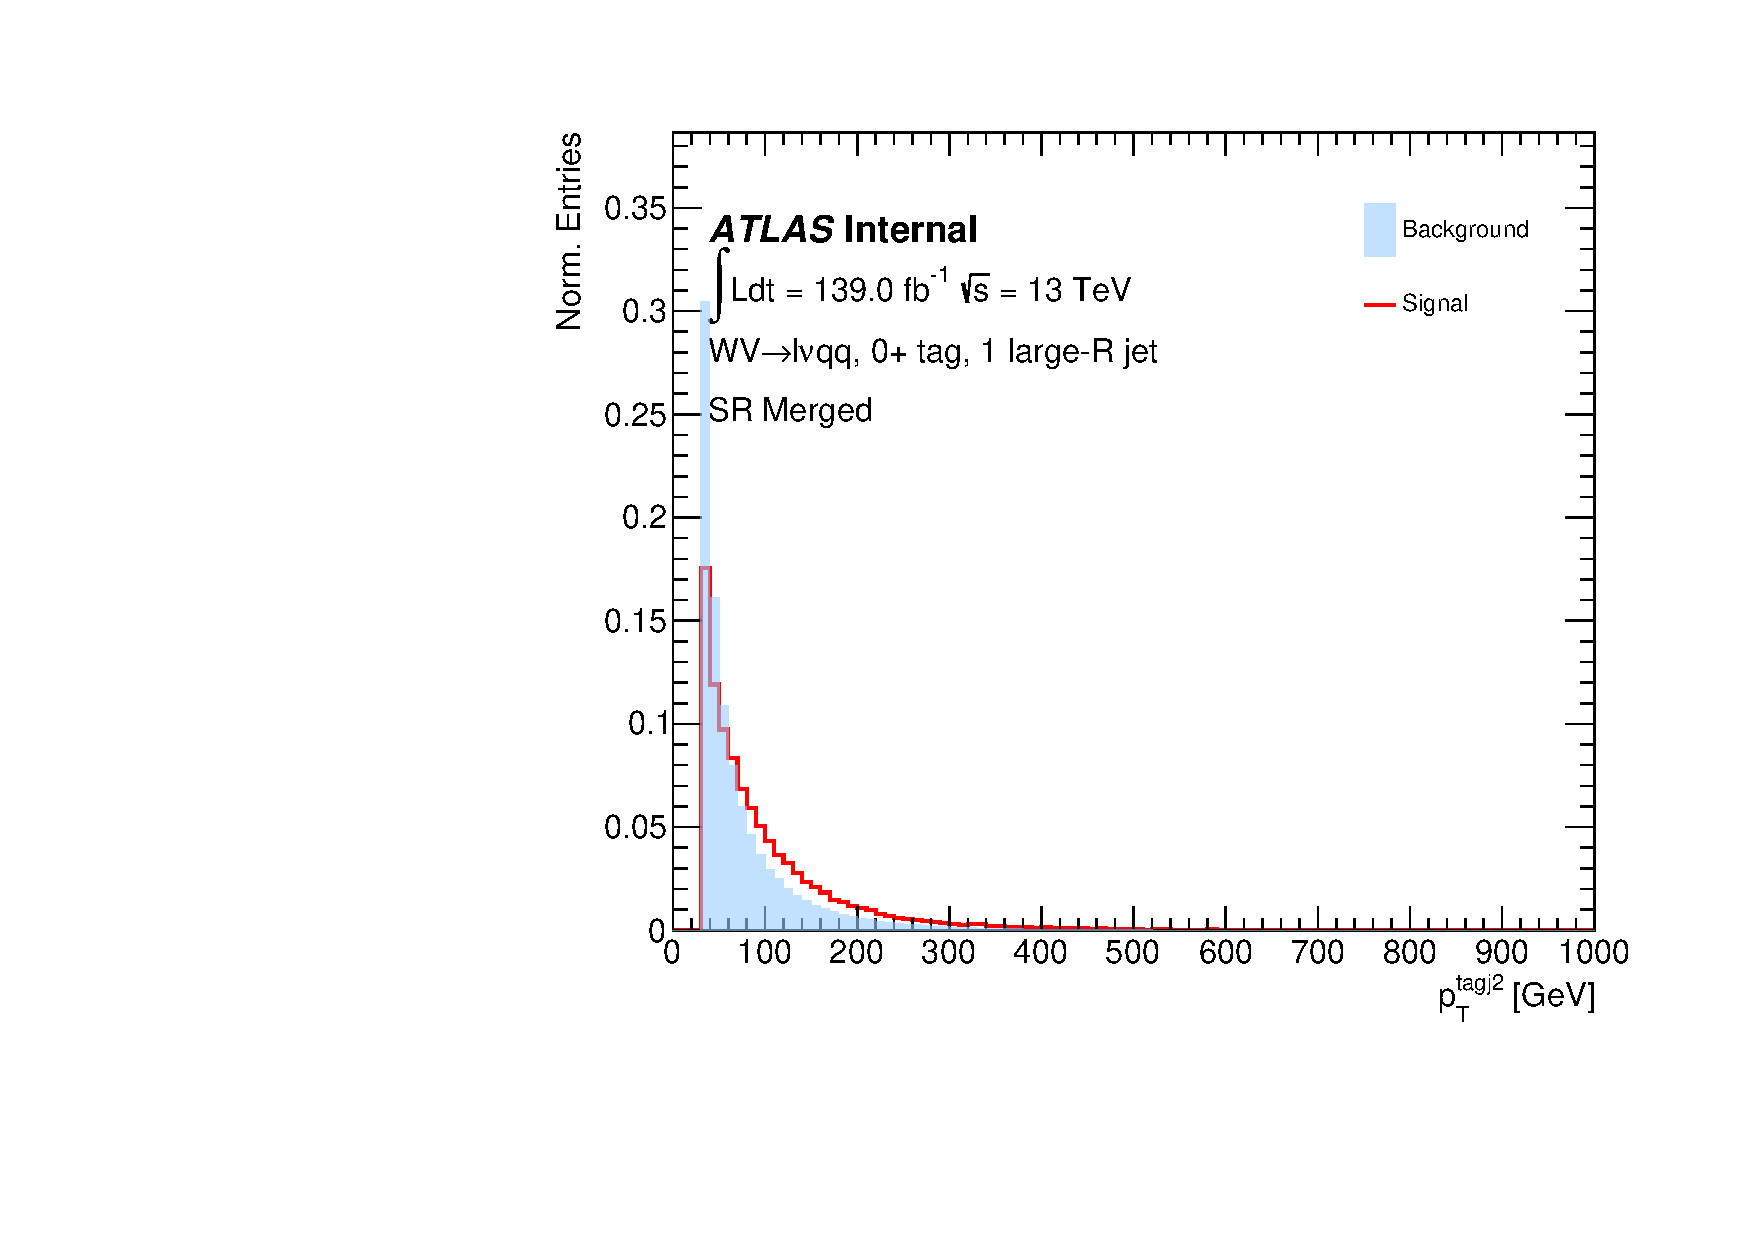
\includegraphics[width=0.3\textwidth]{figures/ml_dnn/variables/SR_Mer/norm_plot_merged_tagJ2_pt.pdf}}\quad
  \subfloat[]{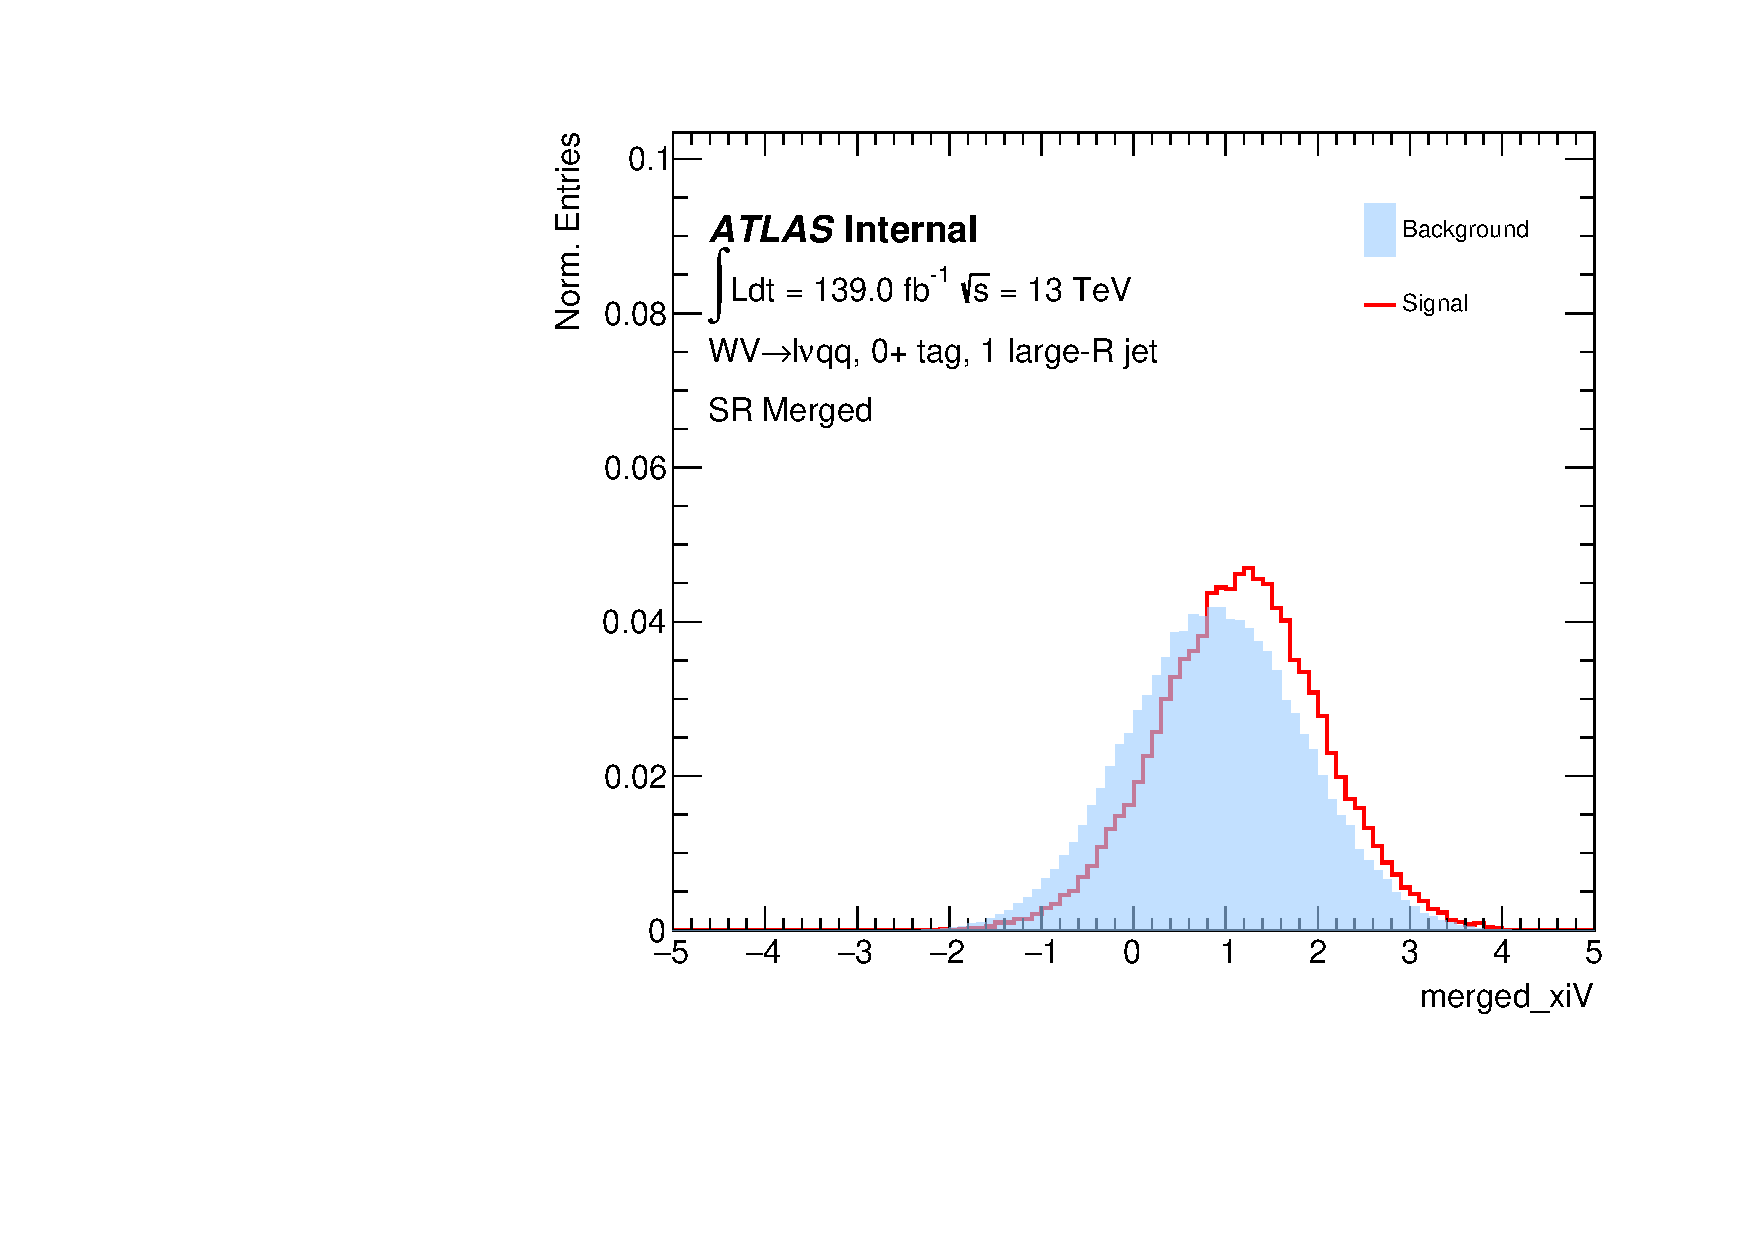
\includegraphics[width=0.3\textwidth]{figures/ml_dnn/variables/SR_Mer/norm_plot_merged_xiV.pdf}}\quad
  \subfloat[]{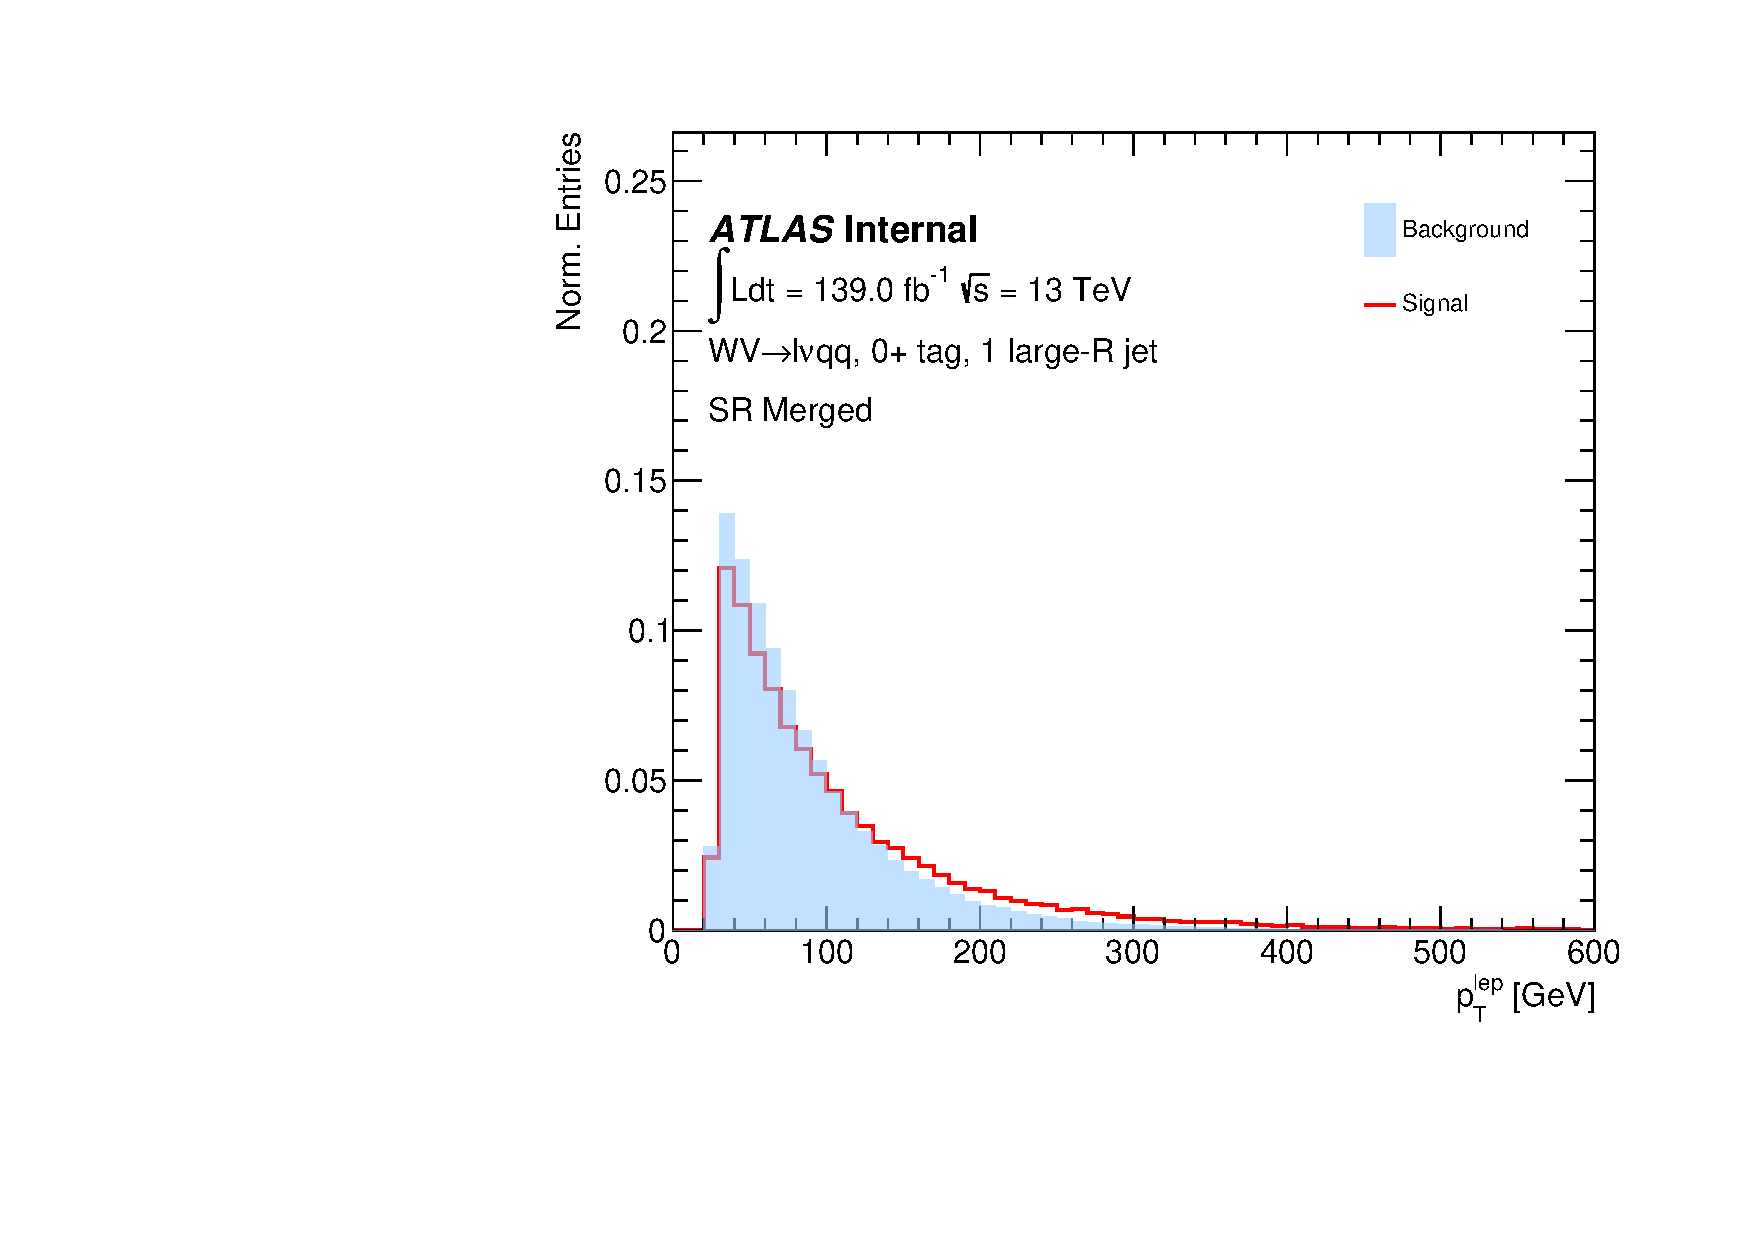
\includegraphics[width=0.3\textwidth]{figures/ml_dnn/variables/SR_Mer/norm_plot_lep_pt.pdf}}

  % Row 4
  \subfloat[]{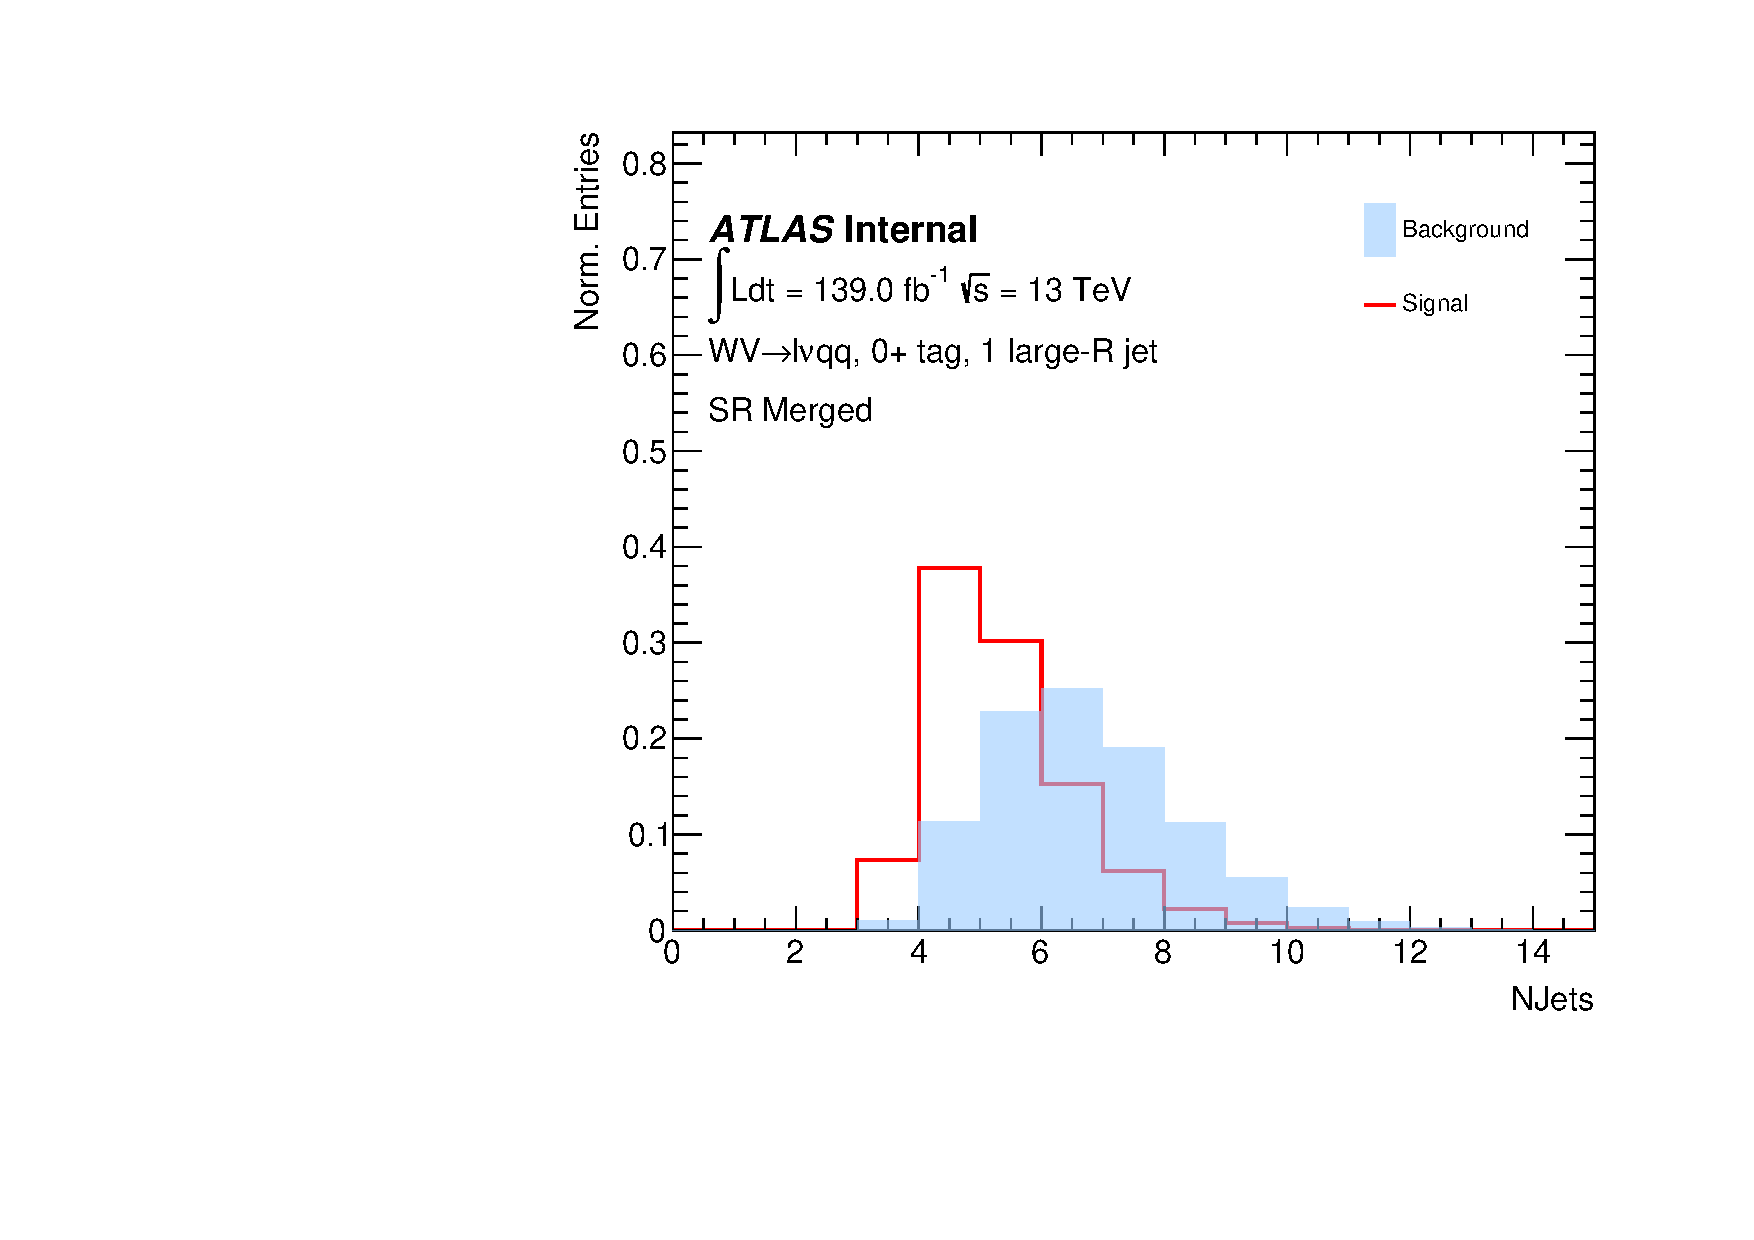
\includegraphics[width=0.3\textwidth]{figures/ml_dnn/variables/SR_Mer/norm_plot_NJets.pdf}}\quad
  \subfloat[]{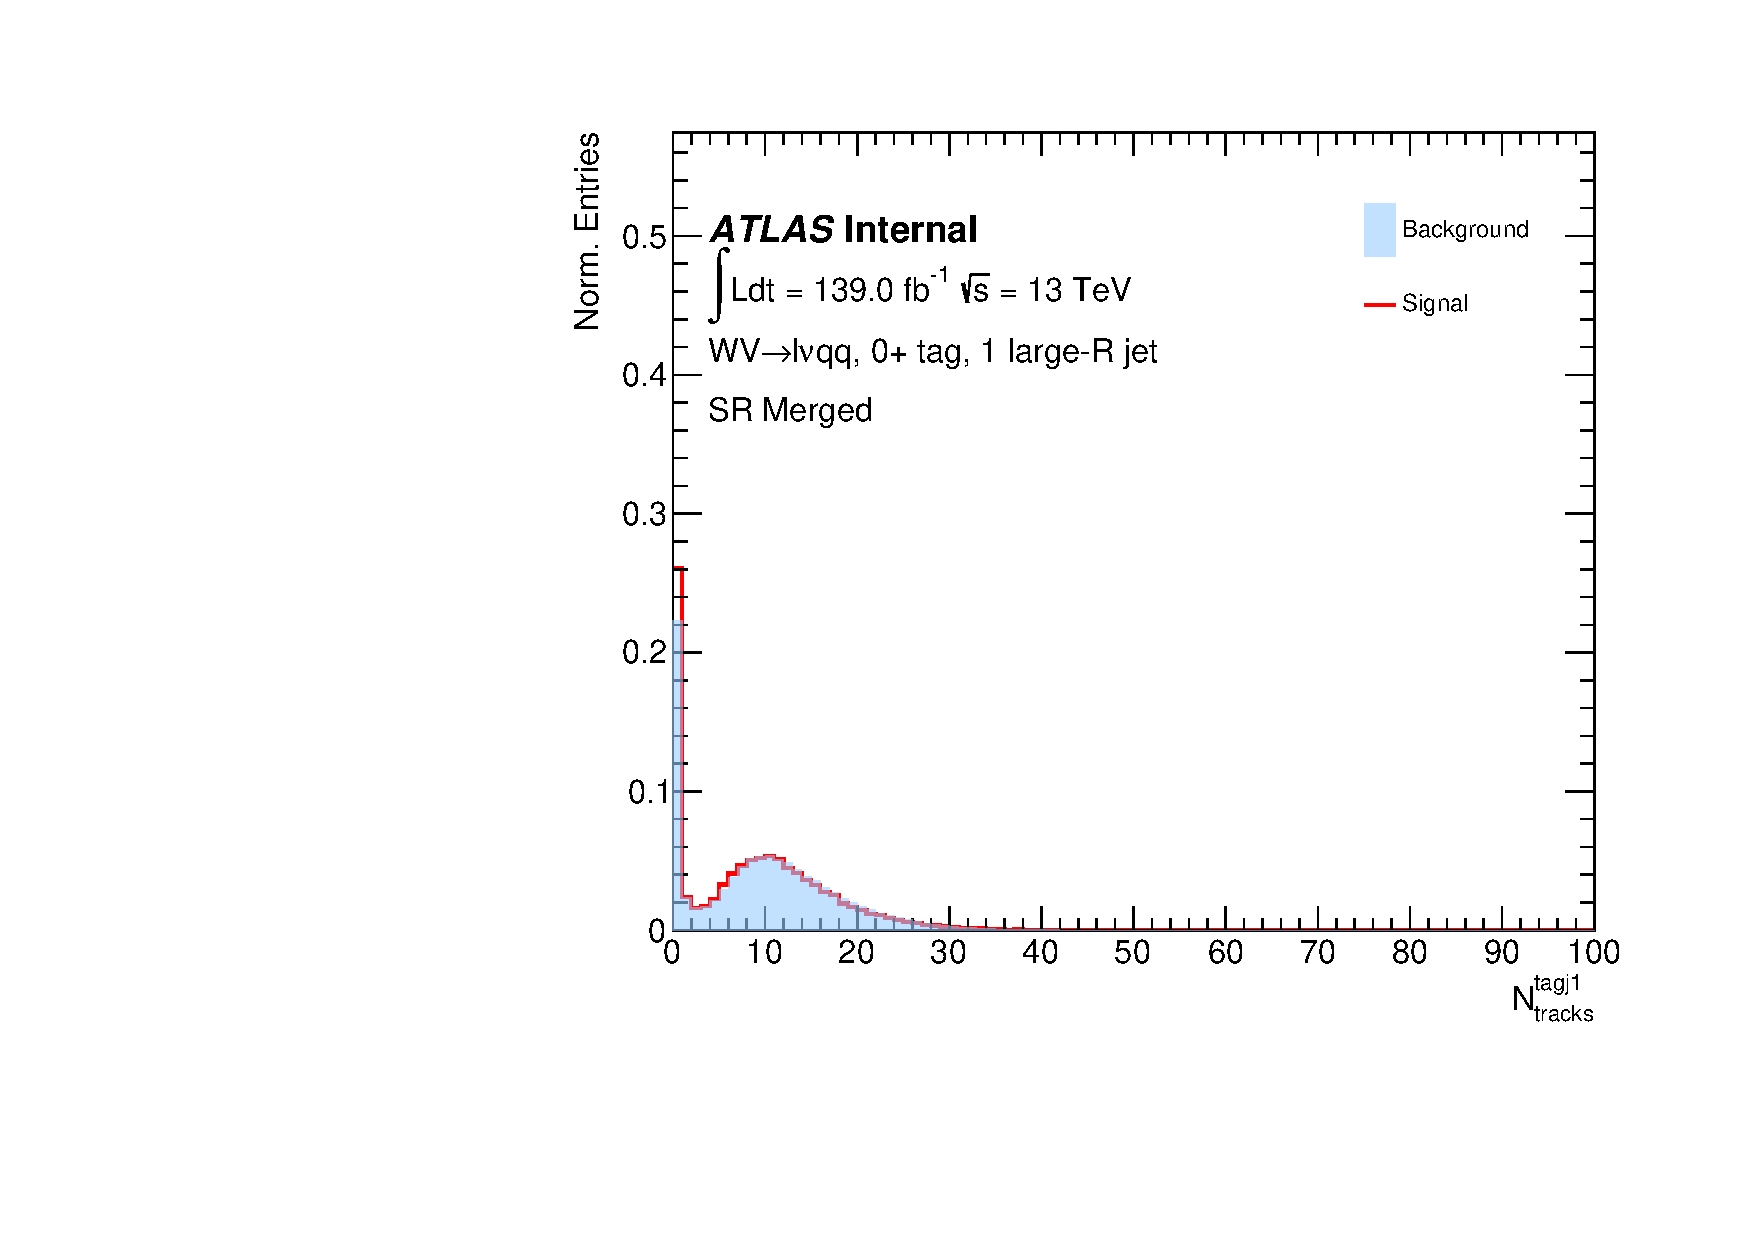
\includegraphics[width=0.3\textwidth]{figures/ml_dnn/variables/SR_Mer/norm_plot_merged_tagJ1_nTracks.pdf}}\quad
  \subfloat[]{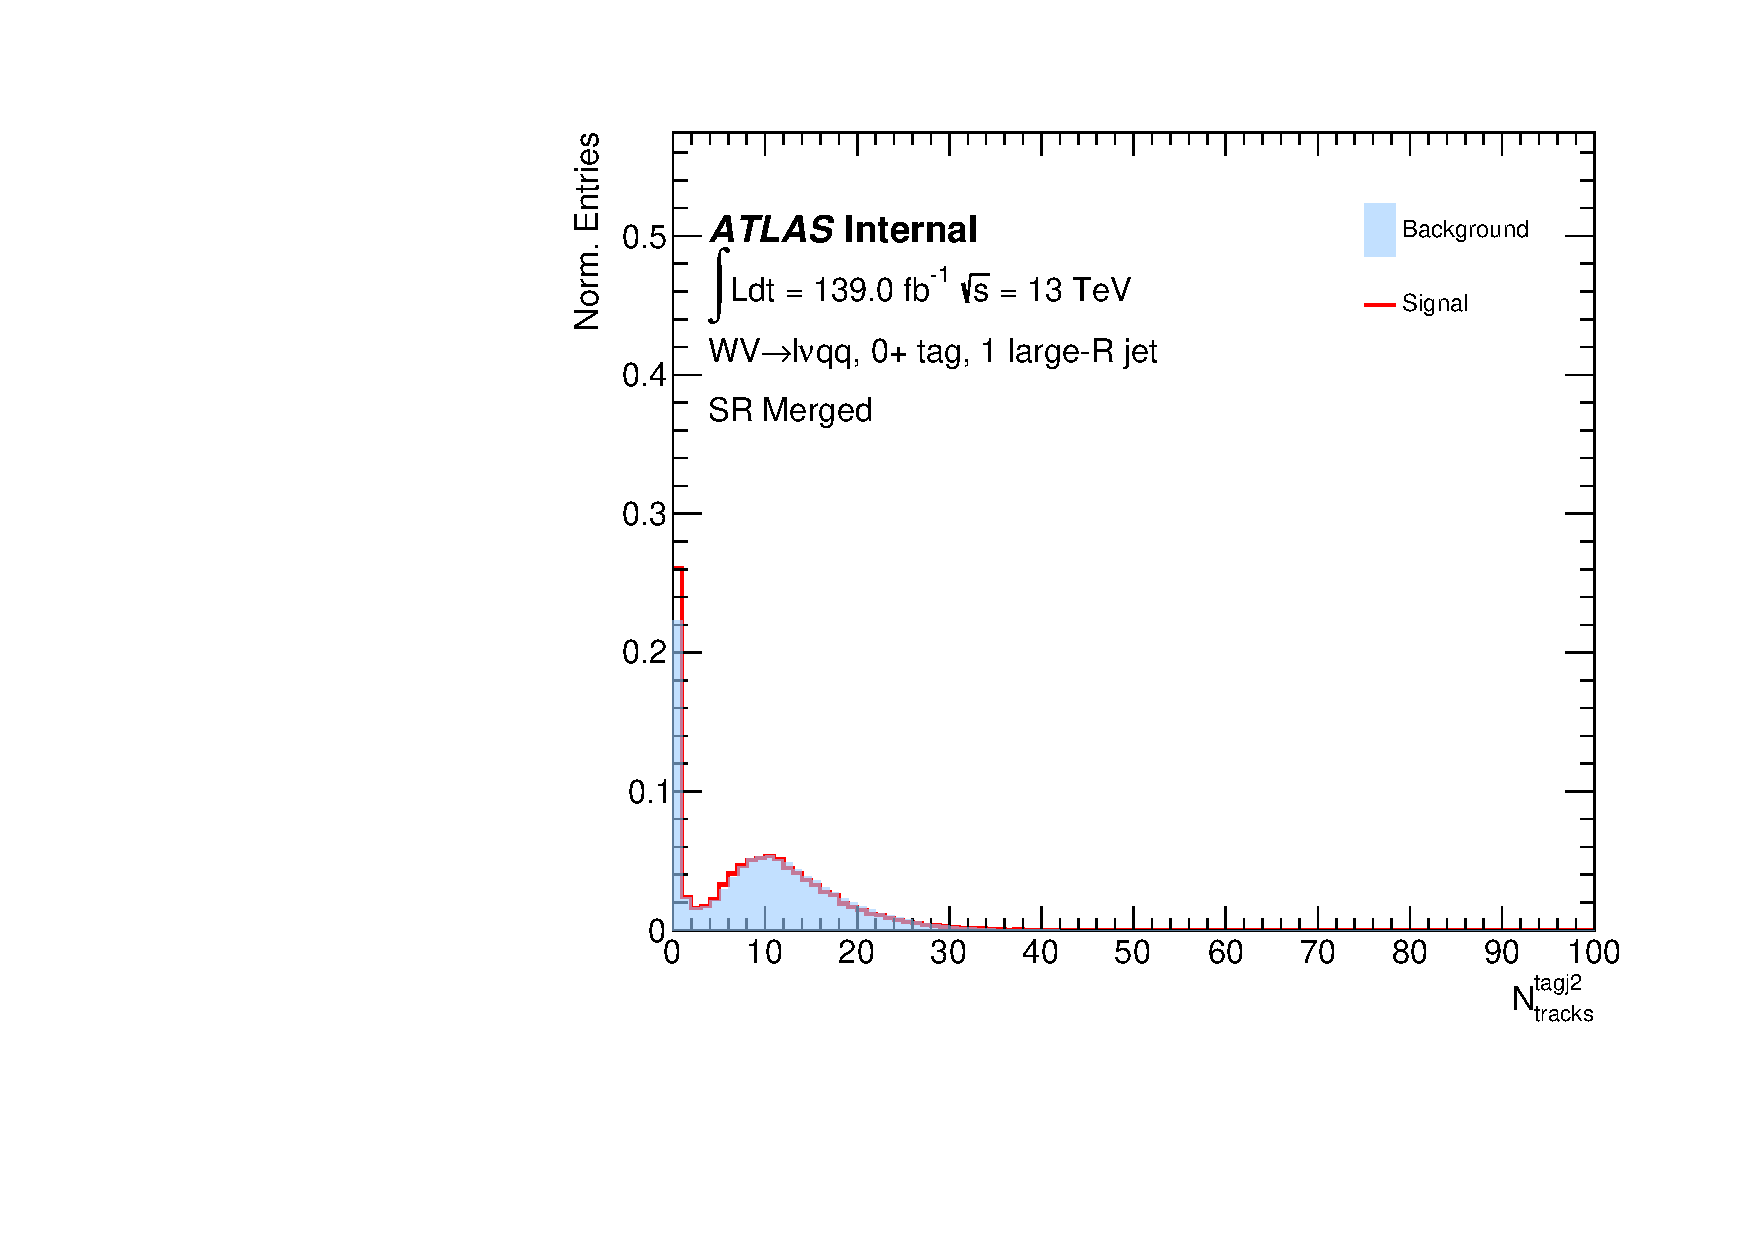
\includegraphics[width=0.3\textwidth]{figures/ml_dnn/variables/SR_Mer/norm_plot_merged_tagJ2_nTracks.pdf}}

  % Row 5
  \subfloat[]{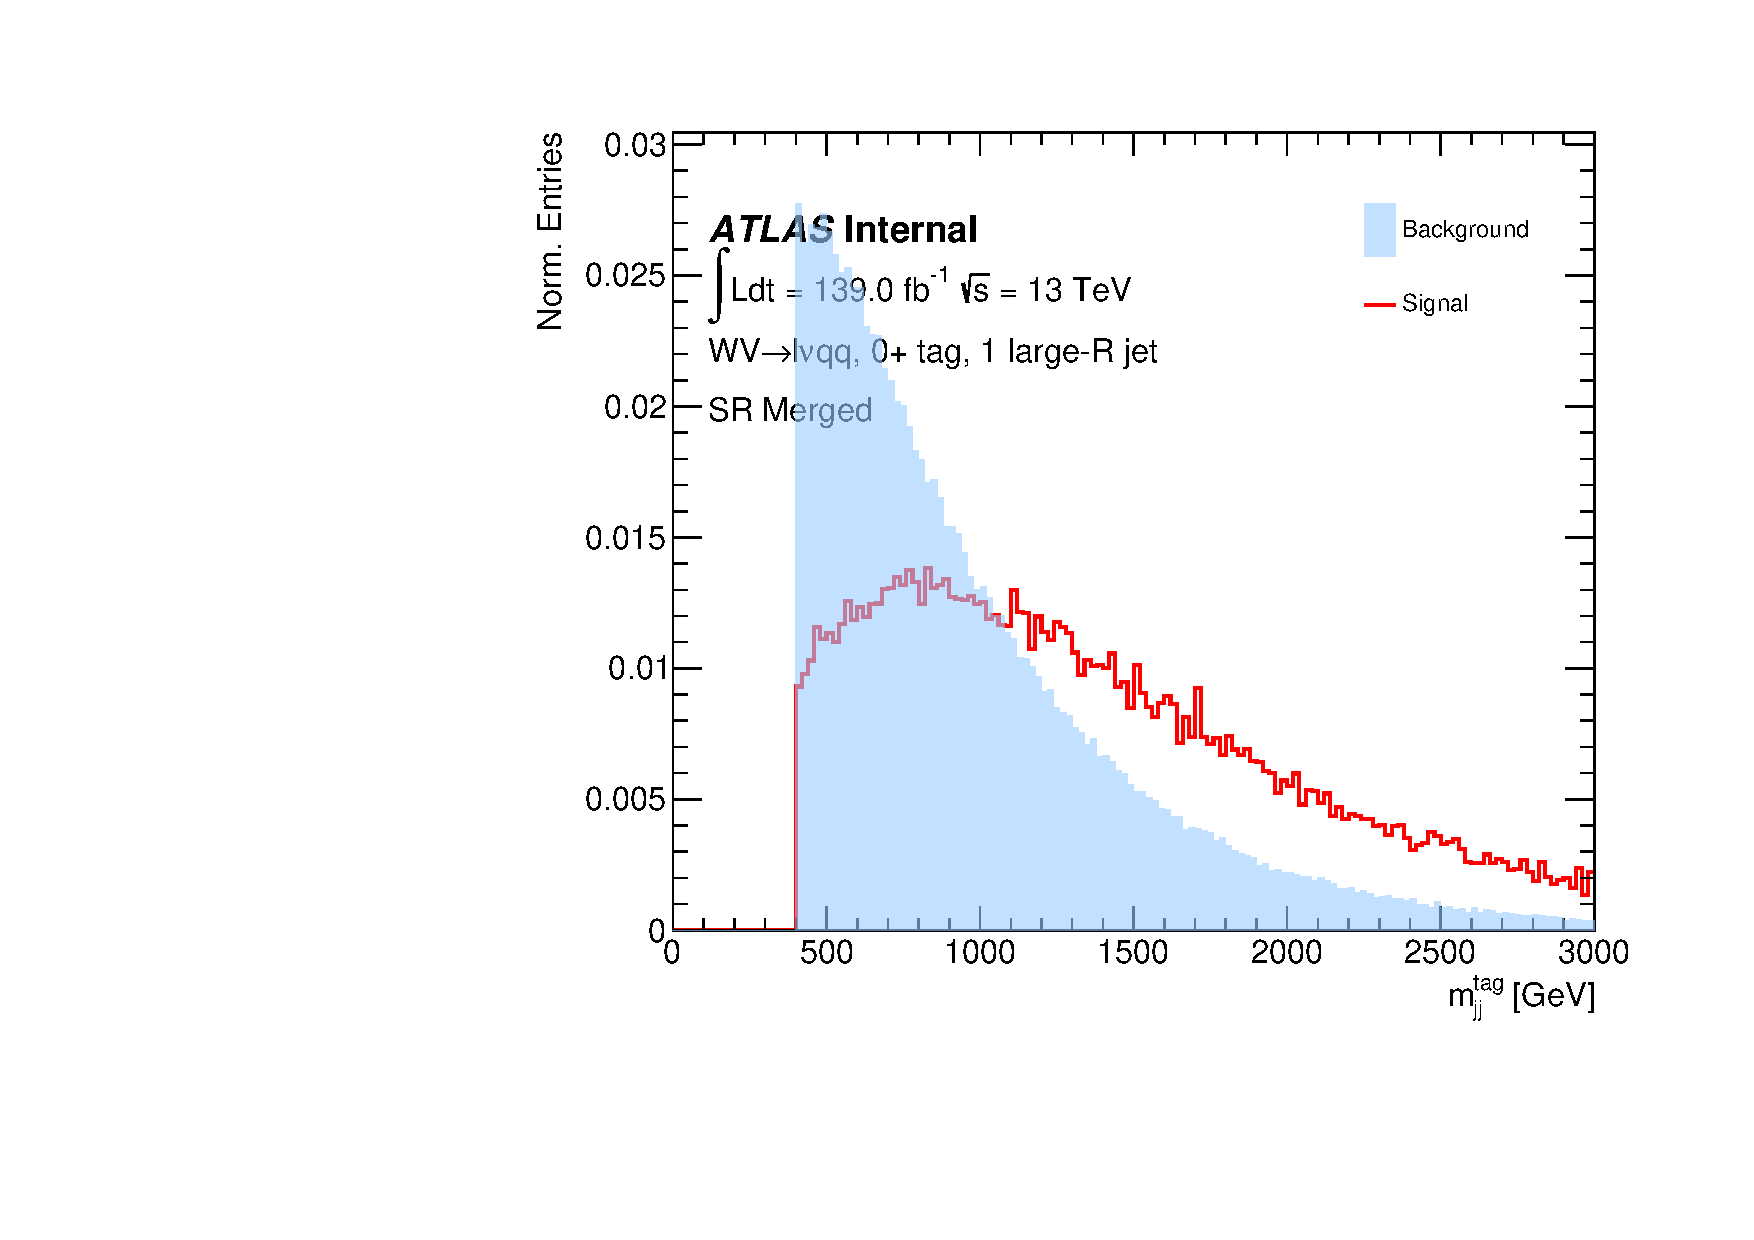
\includegraphics[width=0.3\textwidth]{figures/ml_dnn/variables/SR_Mer/norm_plot_merged_tagMjj.pdf}}\quad
  \subfloat[]{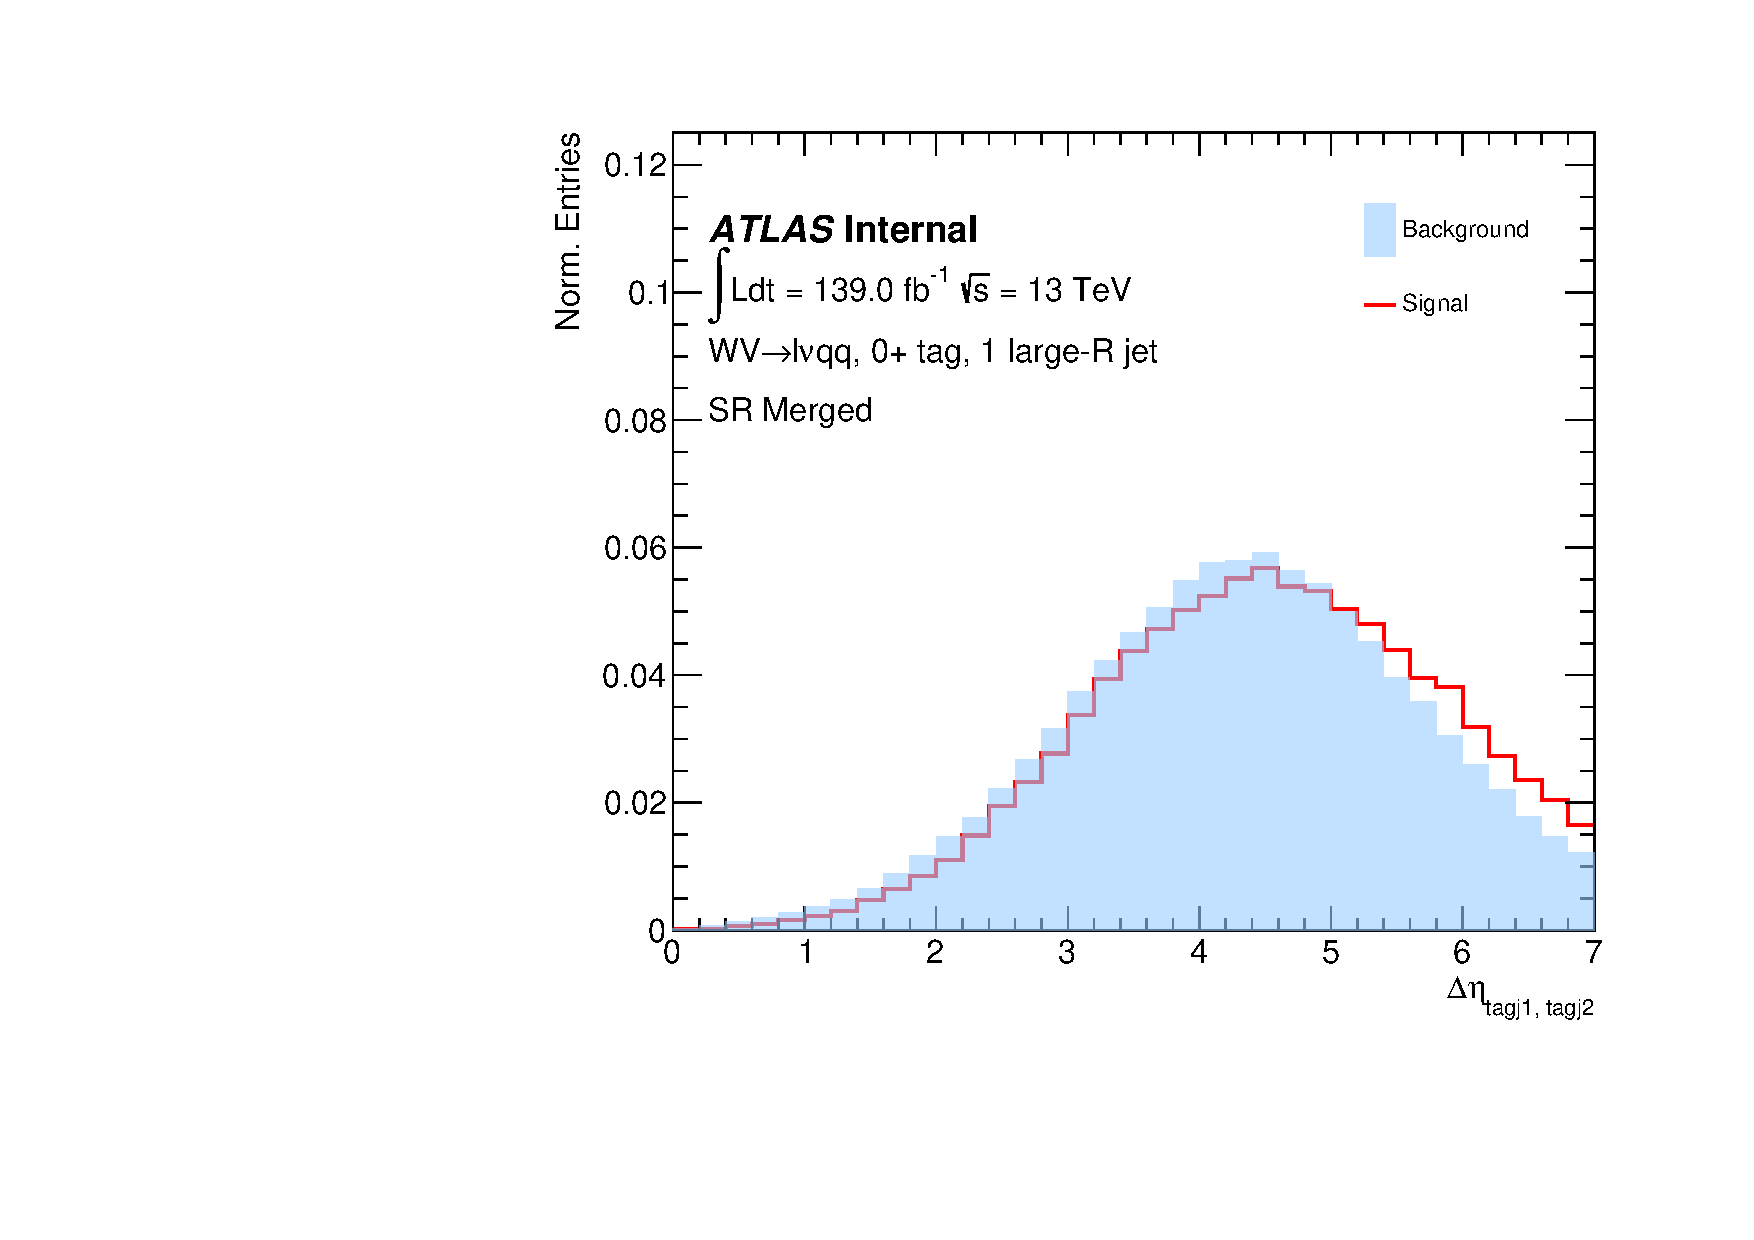
\includegraphics[width=0.3\textwidth]{figures/ml_dnn/variables/SR_Mer/norm_plot_merged_tagJdEta.pdf}}\quad
  \subfloat[]{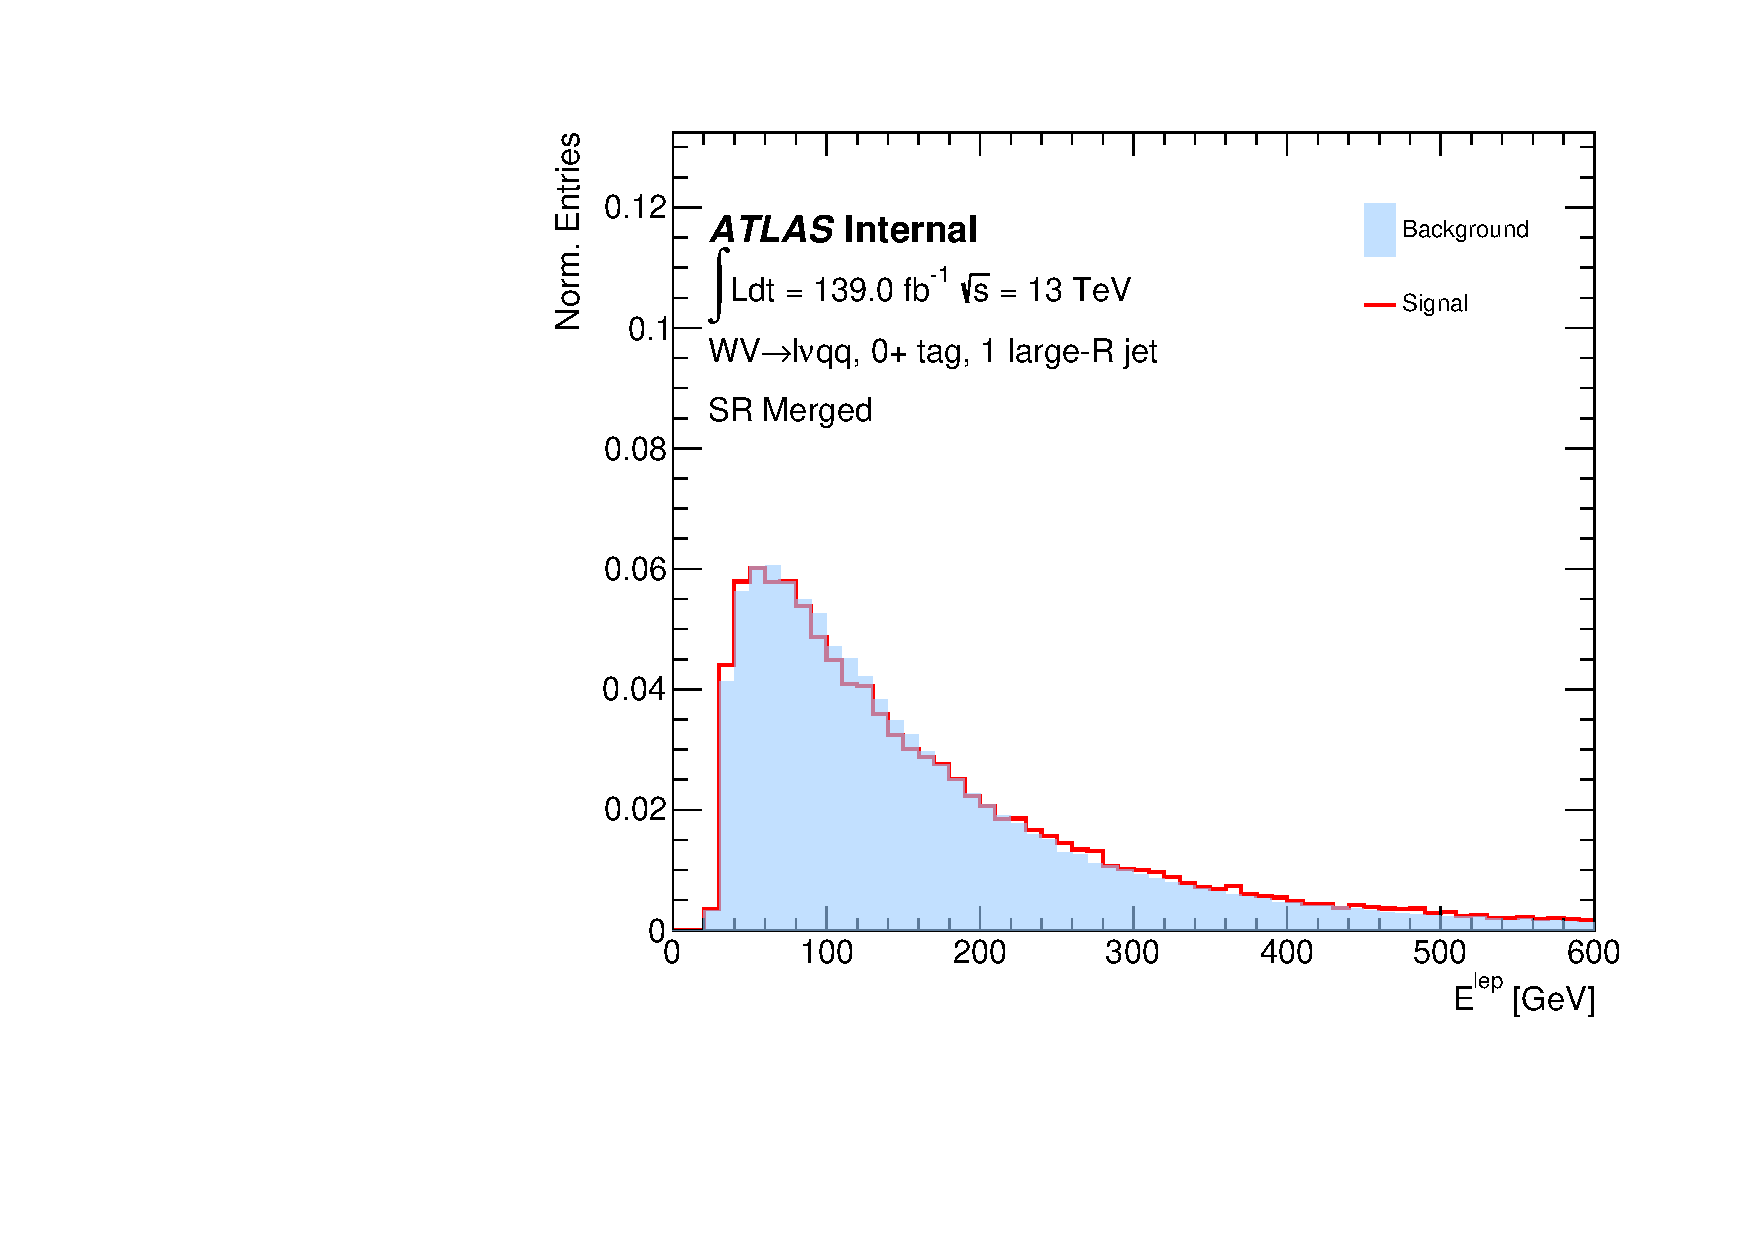
\includegraphics[width=0.3\textwidth]{figures/ml_dnn/variables/SR_Mer/norm_plot_lep_e.pdf}}

 \caption{Distributions of input variables in the Merged SR (Continued)}
 \label{fig:mer_inputs-part2}
\end{figure}

\begin{figure}[ht]
 \centering
  % Row 1
  \subfloat[]{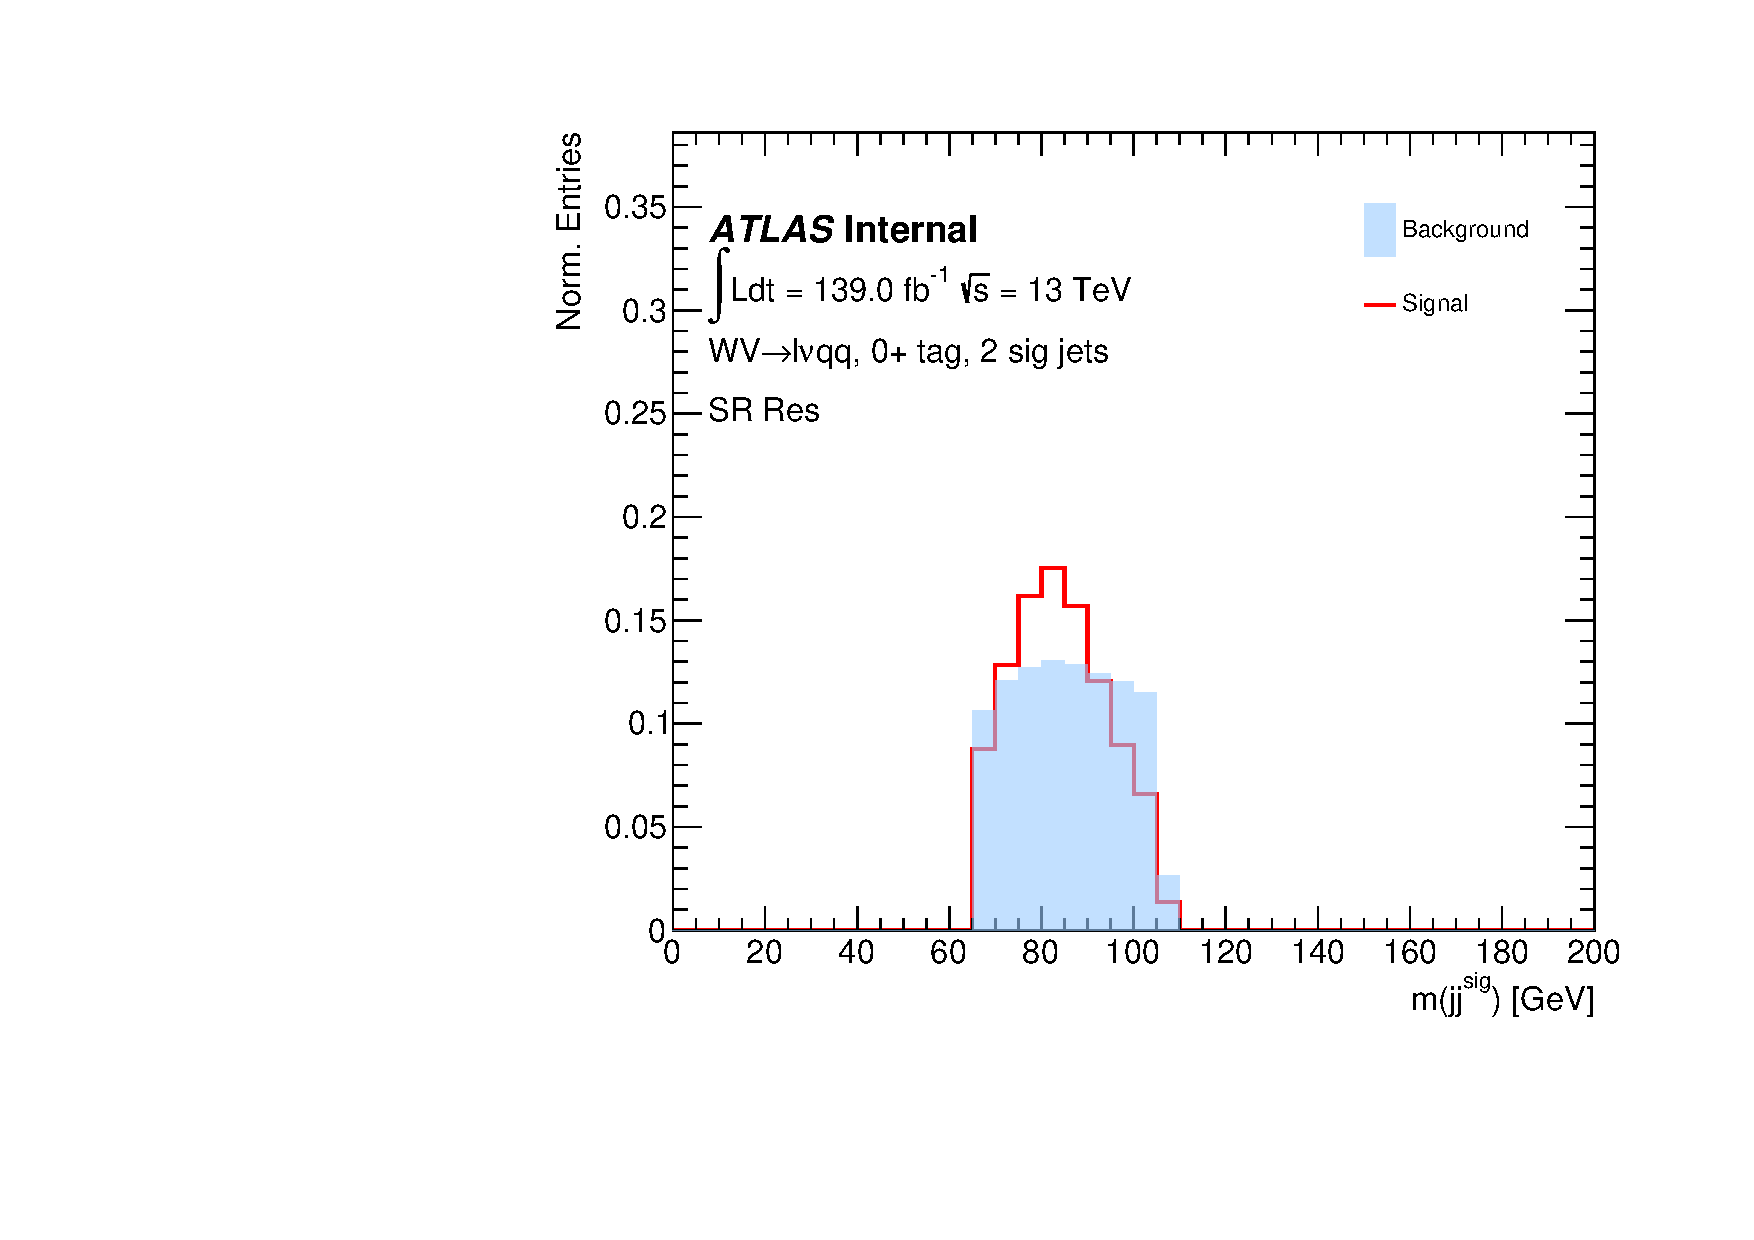
\includegraphics[width=0.3\textwidth]{figures/ml_dnn/variables/SR_Res/norm_plot_Dijet_m.pdf}}\quad
  \subfloat[]{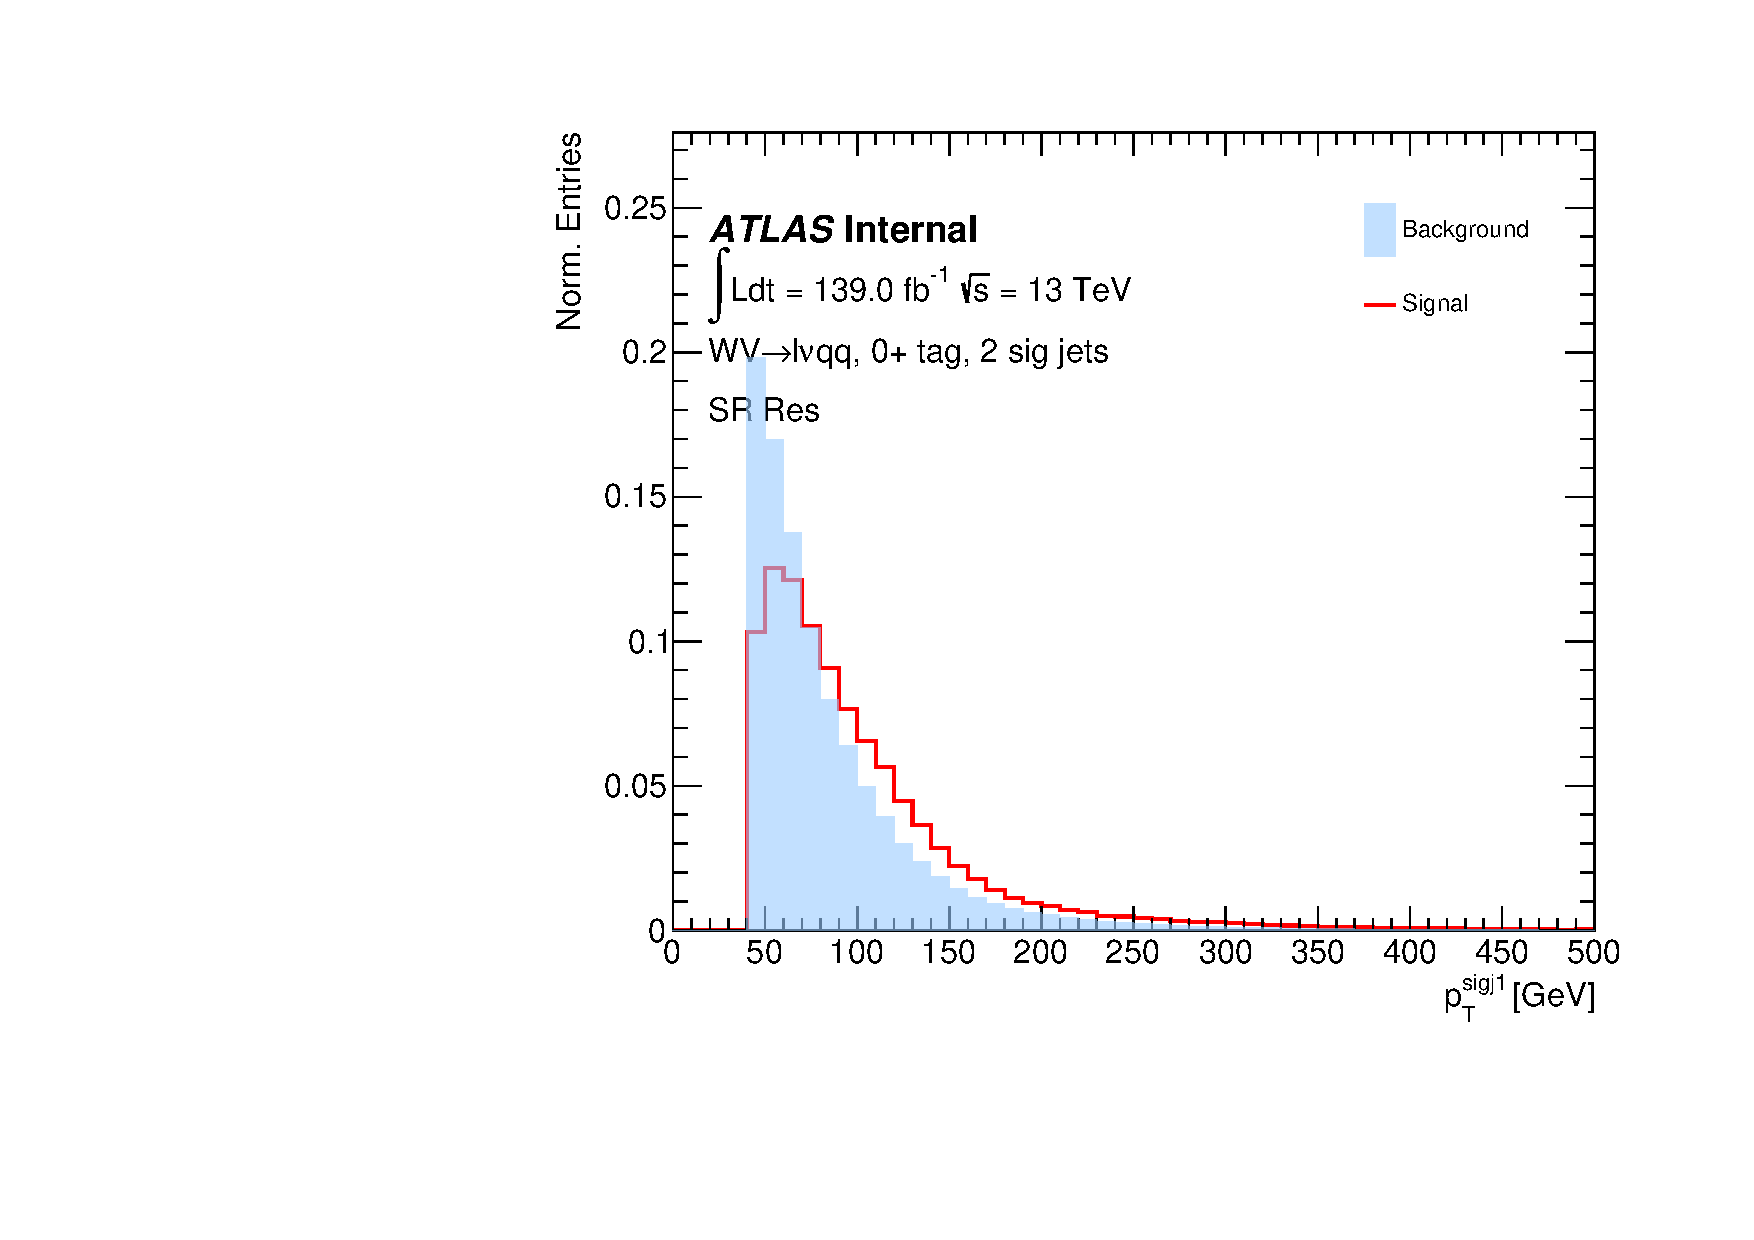
\includegraphics[width=0.3\textwidth]{figures/ml_dnn/variables/SR_Res/norm_plot_sigJ1_pt.pdf}}\quad
  \subfloat[]{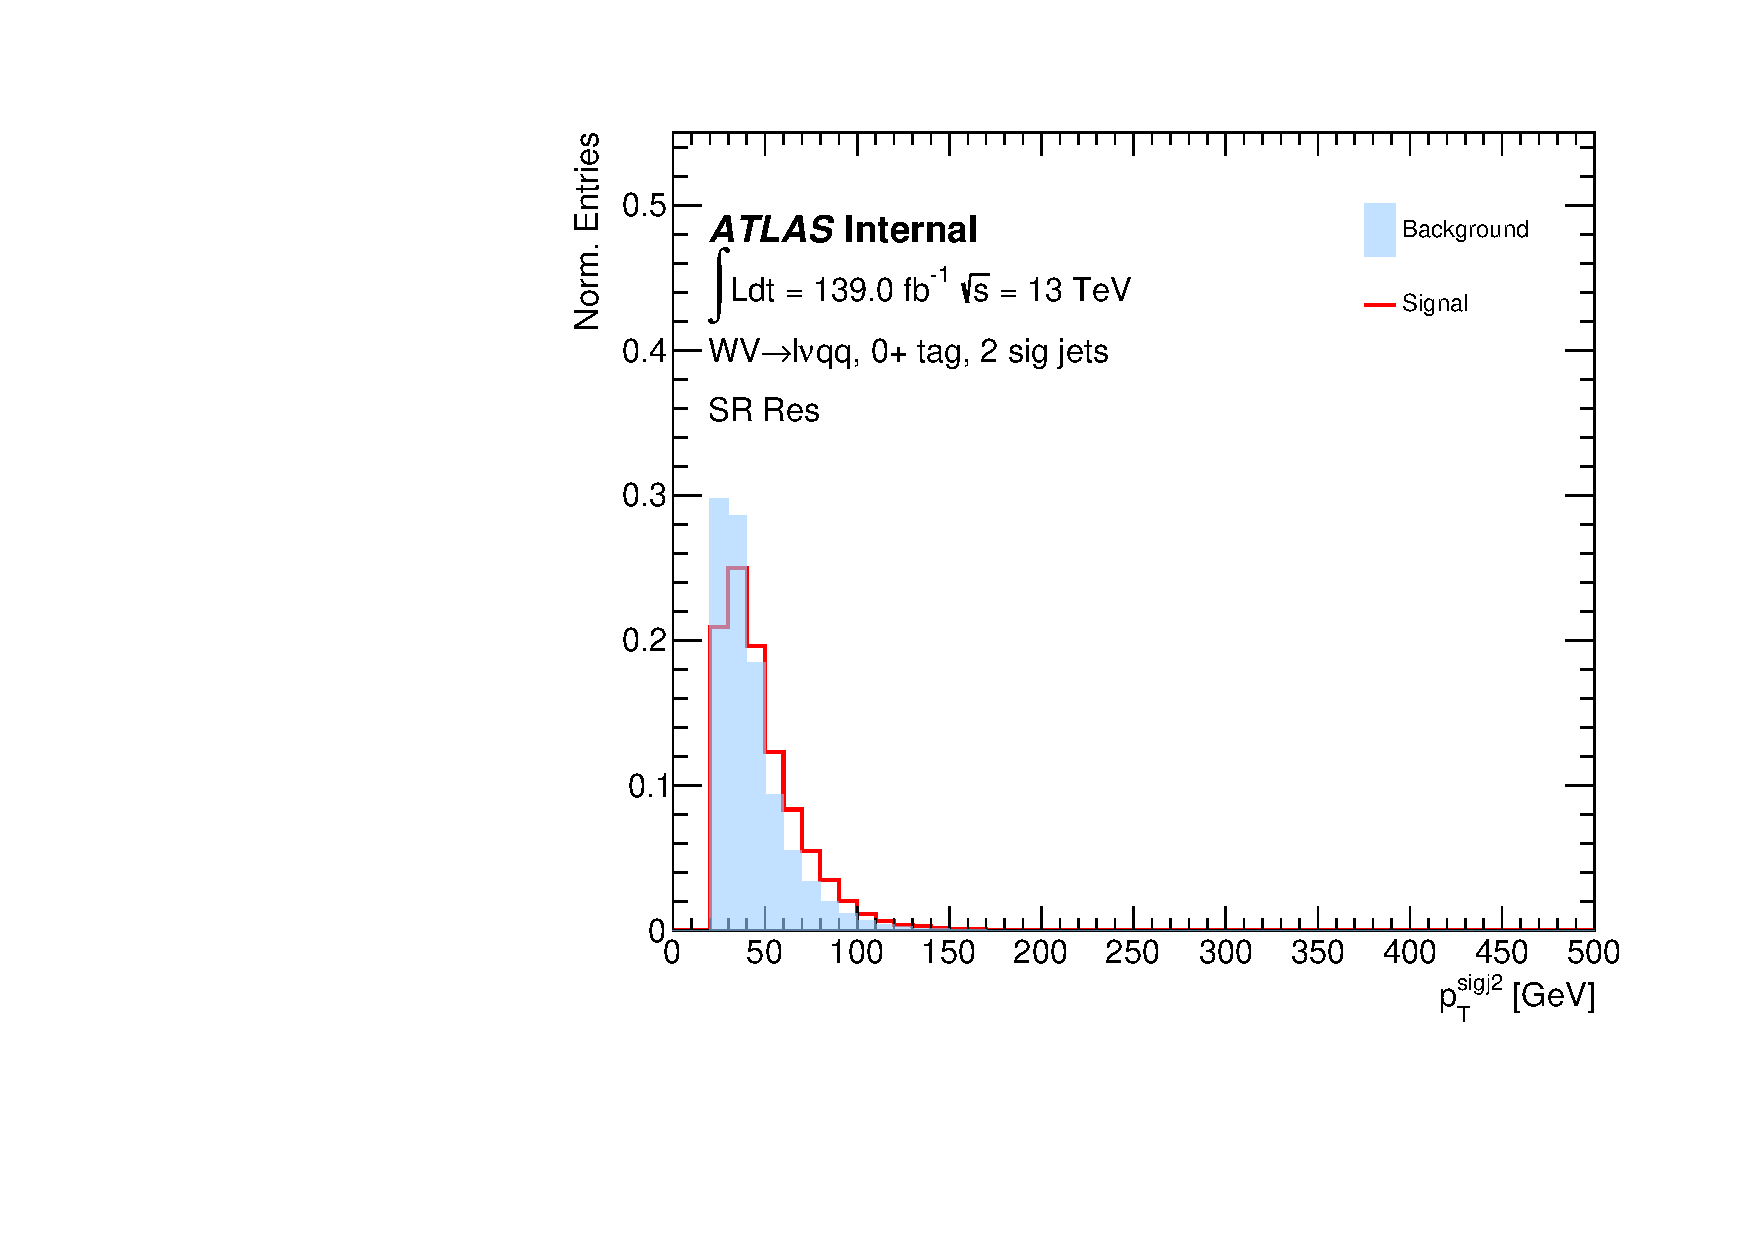
\includegraphics[width=0.3\textwidth]{figures/ml_dnn/variables/SR_Res/norm_plot_sigJ2_pt.pdf}}
  
  % Row 2
  \subfloat[]{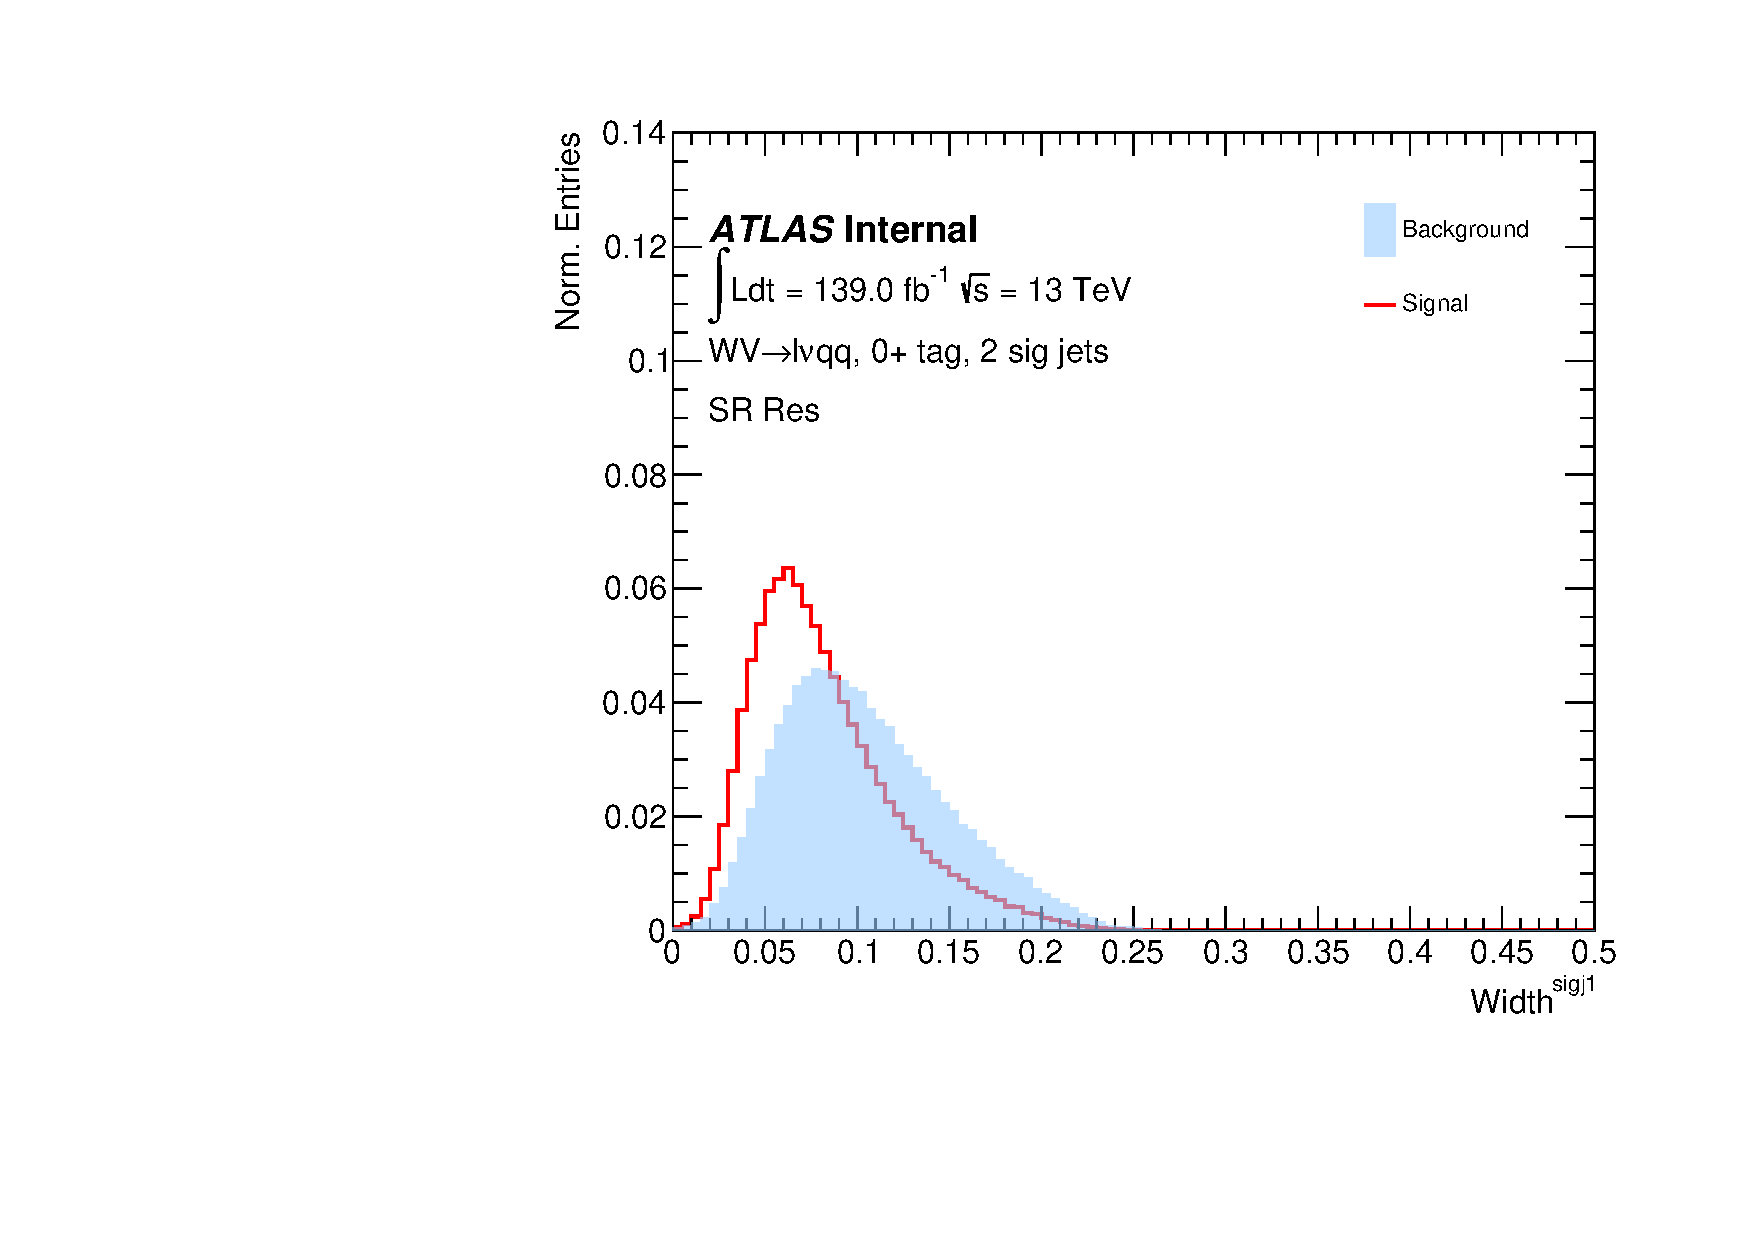
\includegraphics[width=0.3\textwidth]{figures/ml_dnn/variables/SR_Res/norm_plot_sigJ1_width.pdf}}\quad
  \subfloat[]{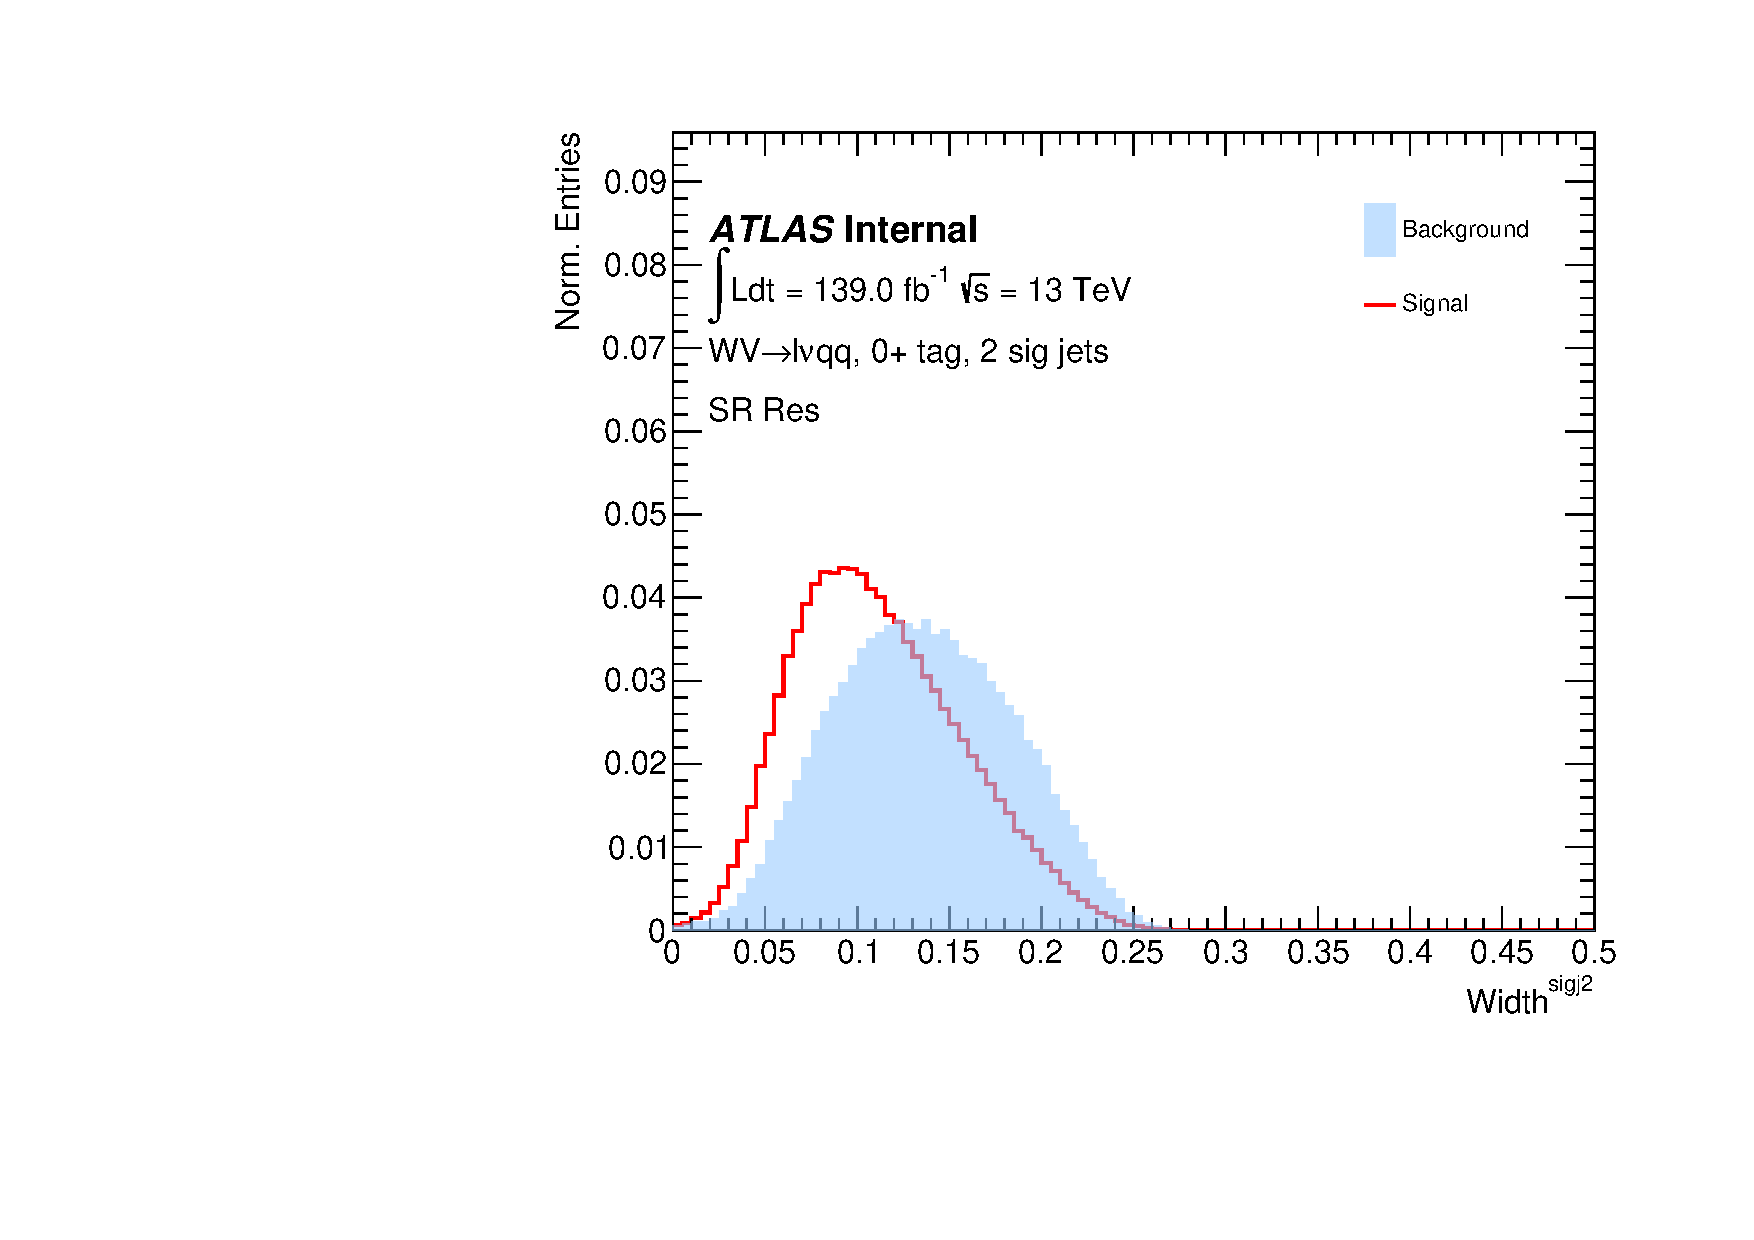
\includegraphics[width=0.3\textwidth]{figures/ml_dnn/variables/SR_Res/norm_plot_sigJ2_width.pdf}}\quad
  \subfloat[]{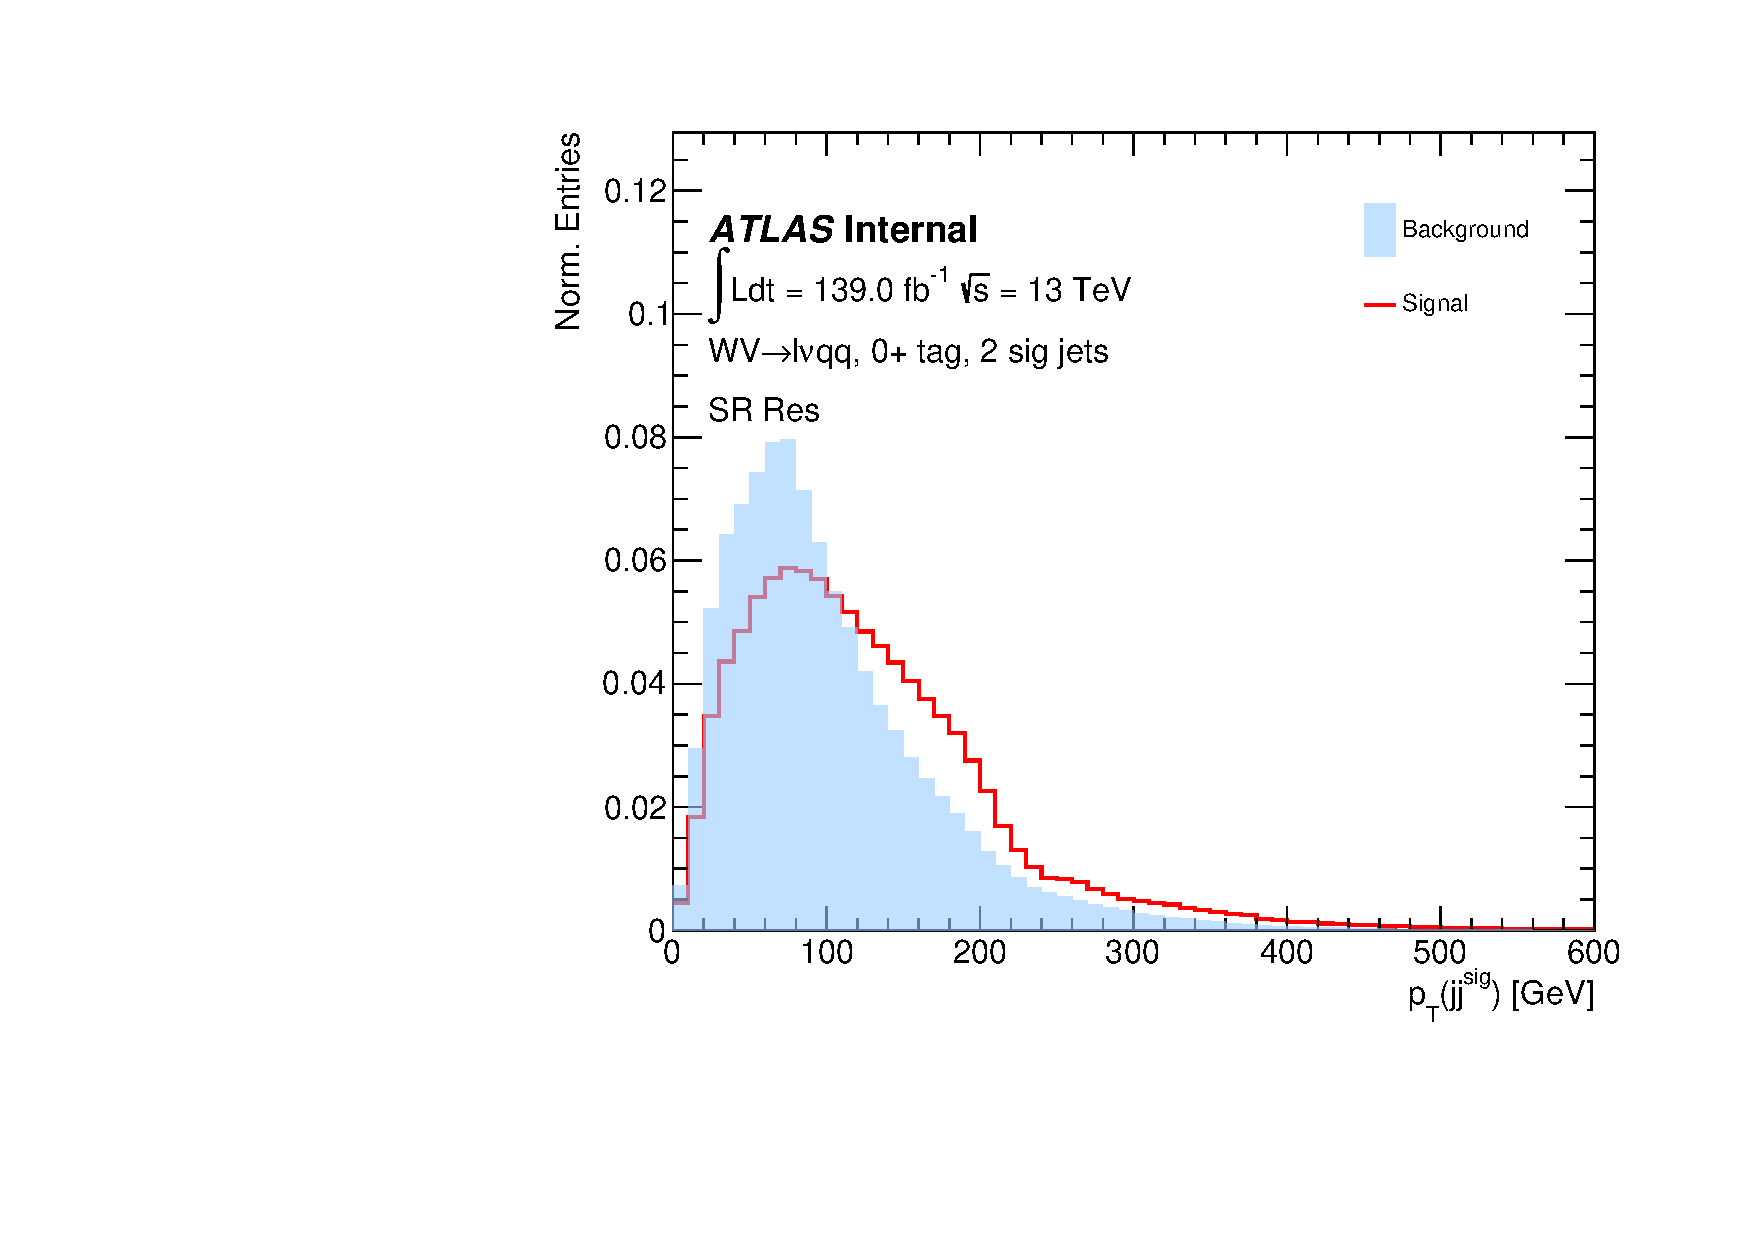
\includegraphics[width=0.3\textwidth]{figures/ml_dnn/variables/SR_Res/norm_plot_Dijet_pt.pdf}}
  
  % Row 3
  \subfloat[]{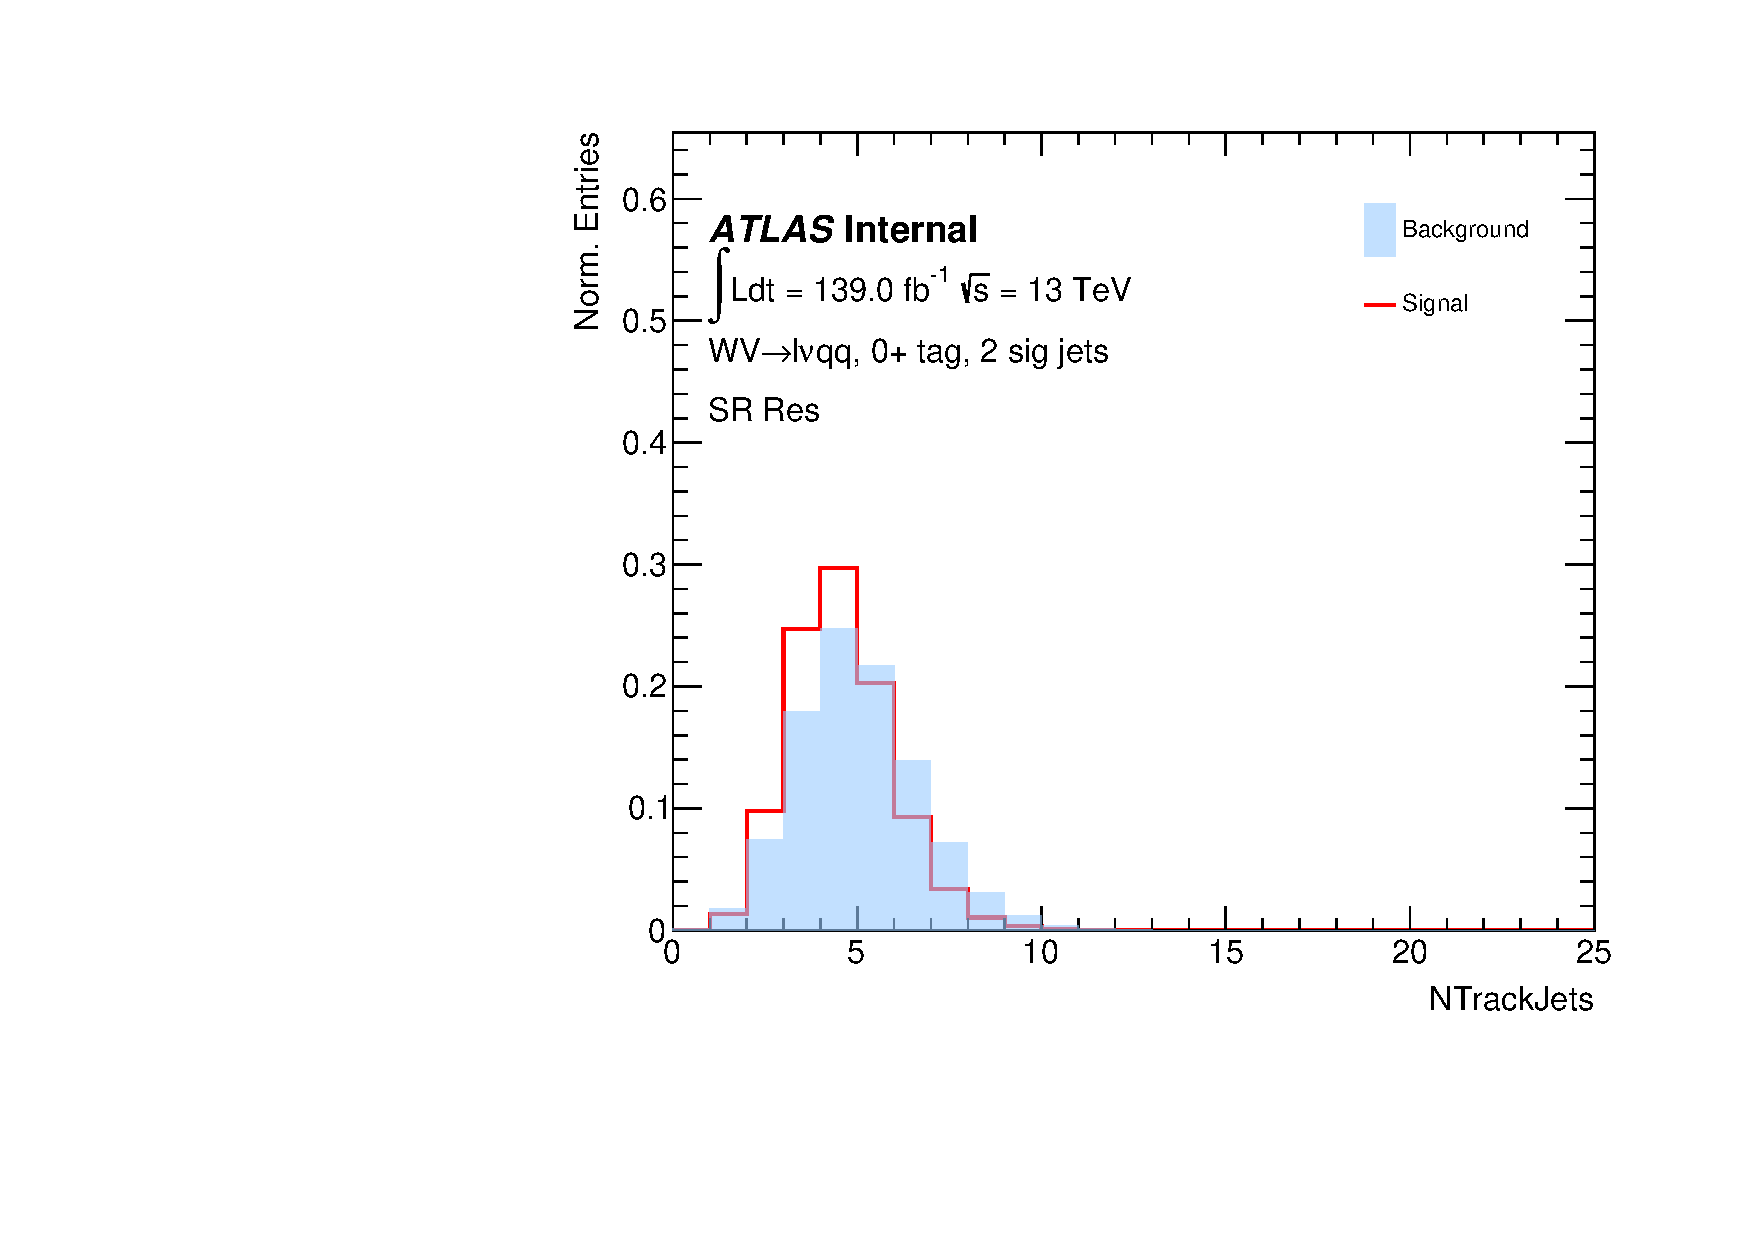
\includegraphics[width=0.3\textwidth]{figures/ml_dnn/variables/SR_Res/norm_plot_NTrackJets.pdf}}\quad
  \subfloat[]{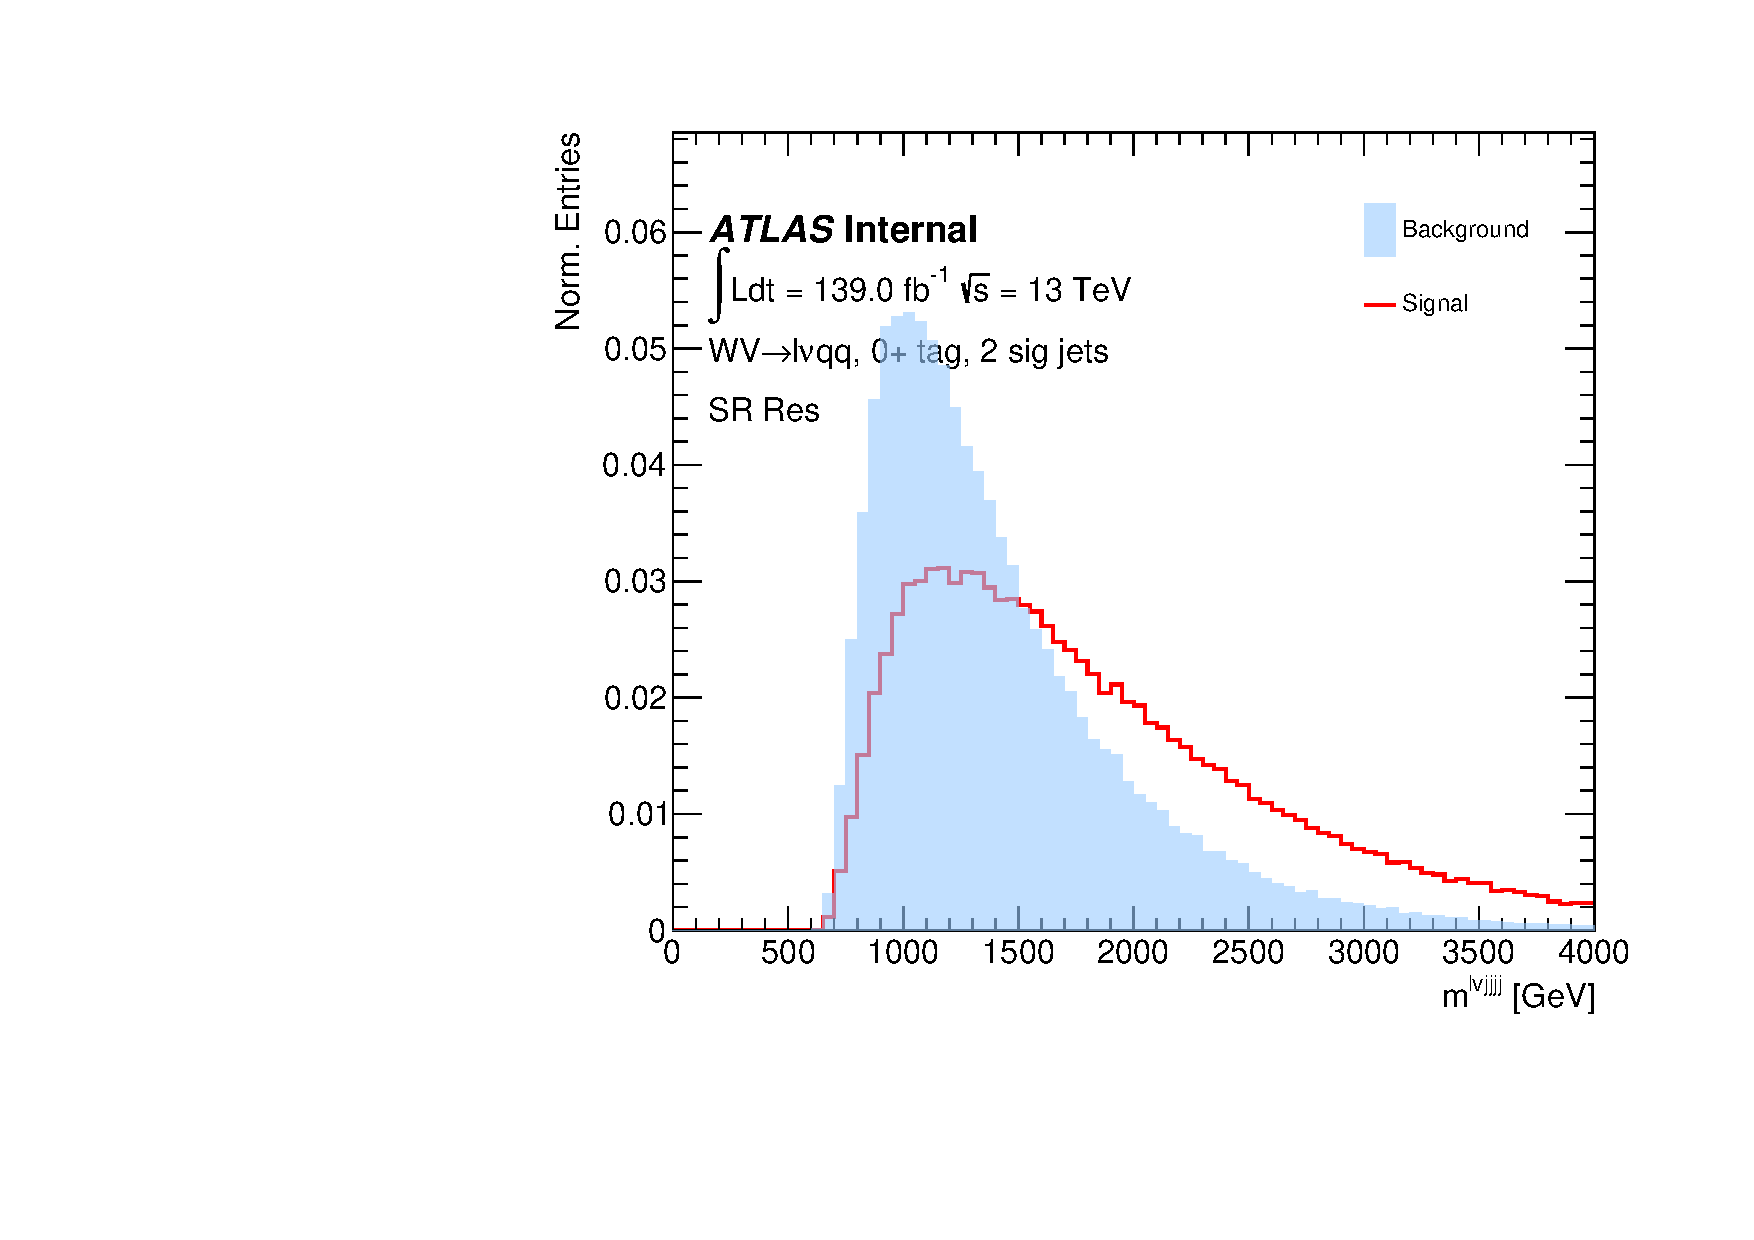
\includegraphics[width=0.3\textwidth]{figures/ml_dnn/variables/SR_Res/norm_plot_lvjjjjmass.pdf}}\quad
  \subfloat[]{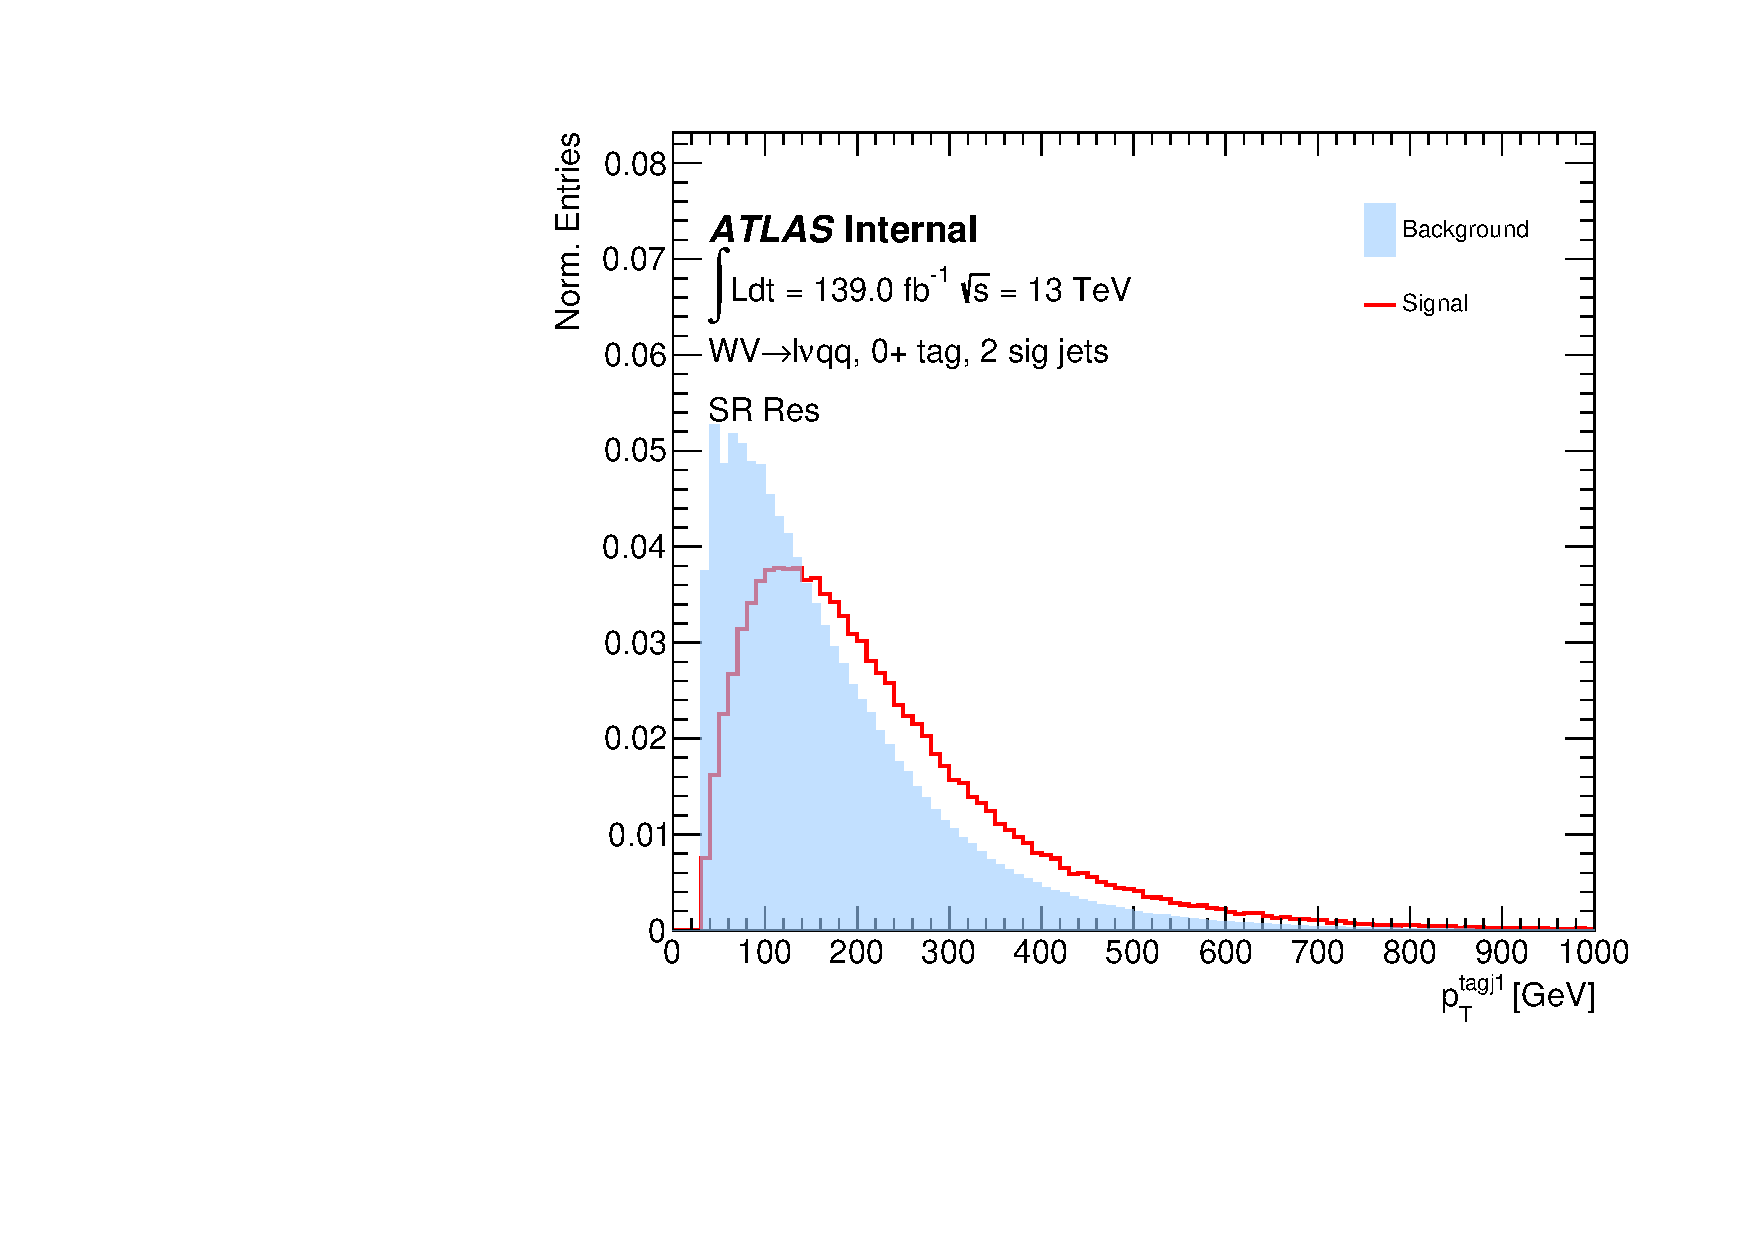
\includegraphics[width=0.3\textwidth]{figures/ml_dnn/variables/SR_Res/norm_plot_resolved_tagJ1_pt.pdf}}
  
 \caption{Distributions of input variables in the Resolved SR (Continued on next page)}
 \label{fig:res_inputs-part1}
\end{figure}

\begin{figure}[ht]
 \centering

  % Row 4
  \subfloat[]{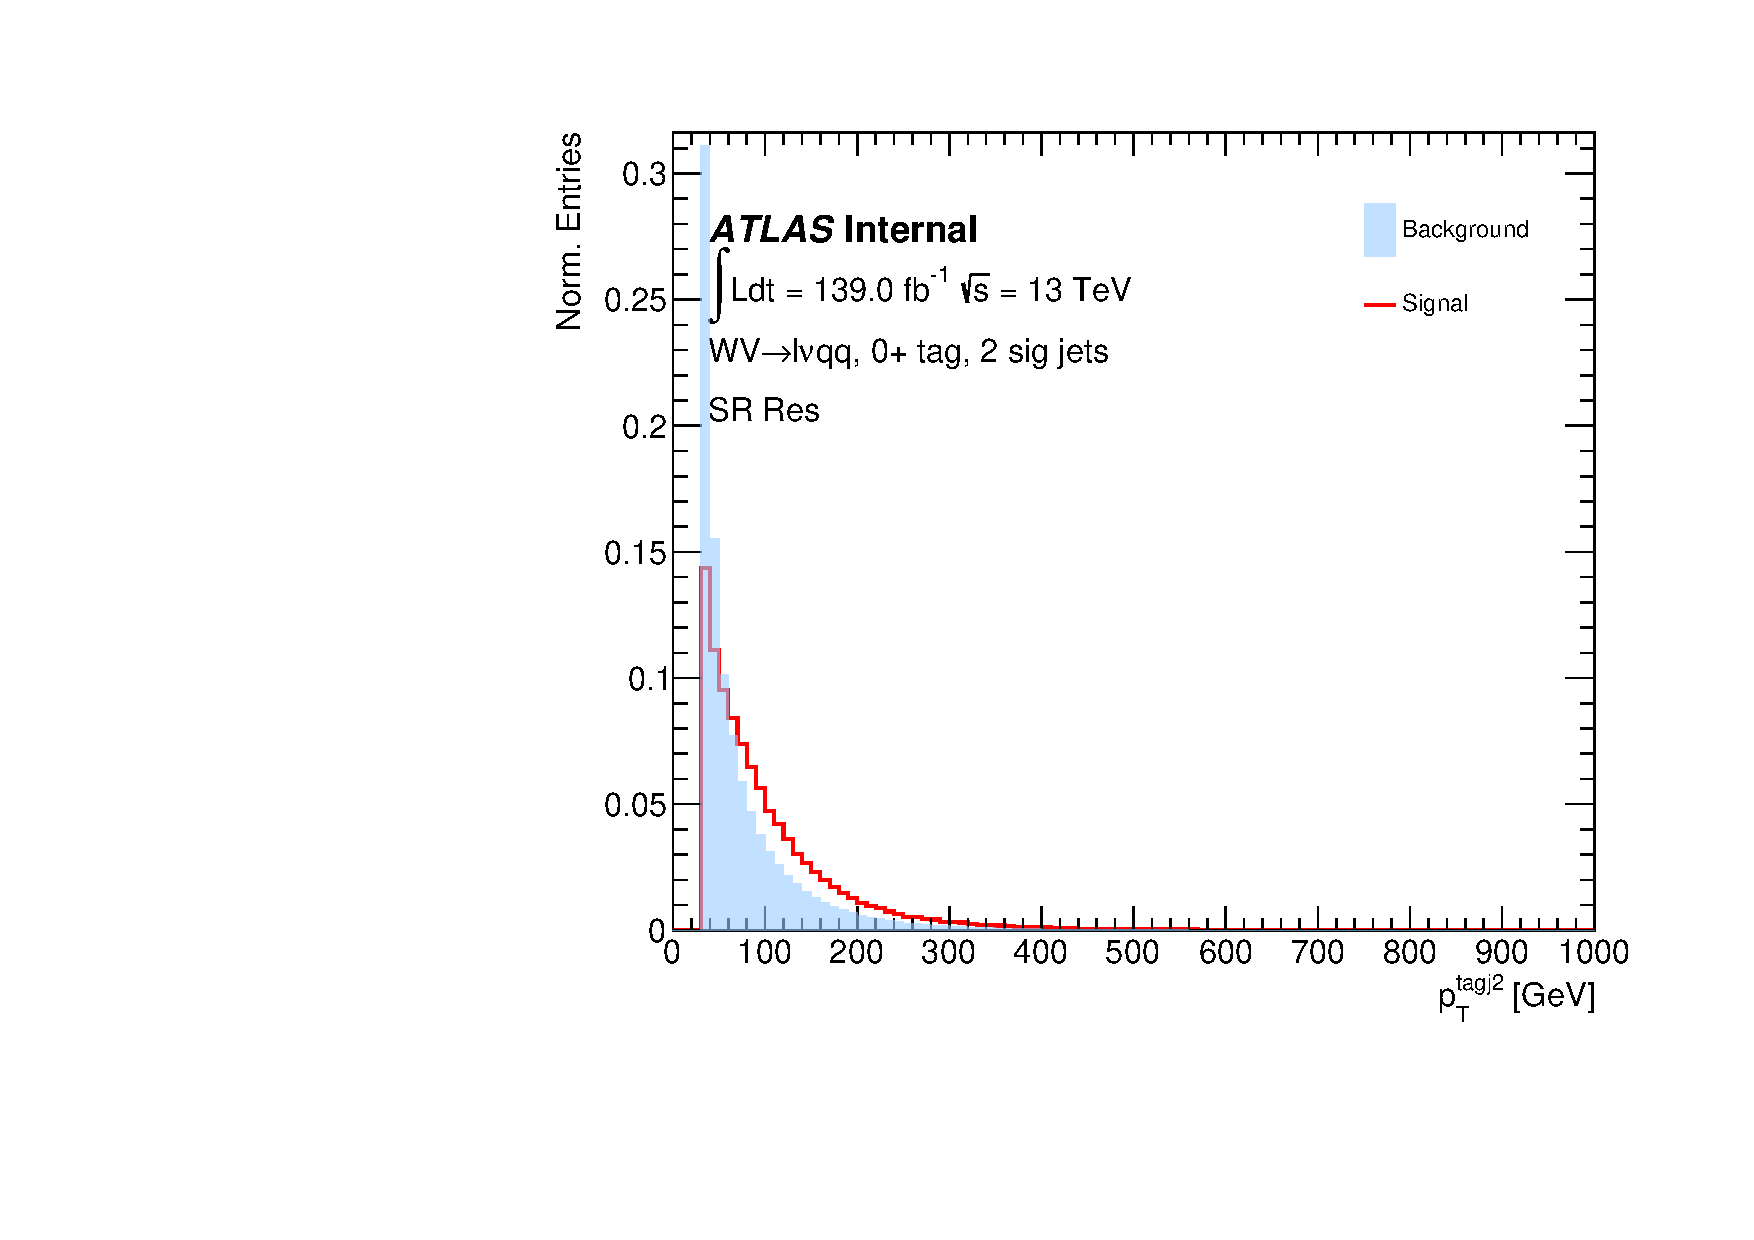
\includegraphics[width=0.3\textwidth]{figures/ml_dnn/variables/SR_Res/norm_plot_resolved_tagJ2_pt.pdf}}\quad
  \subfloat[]{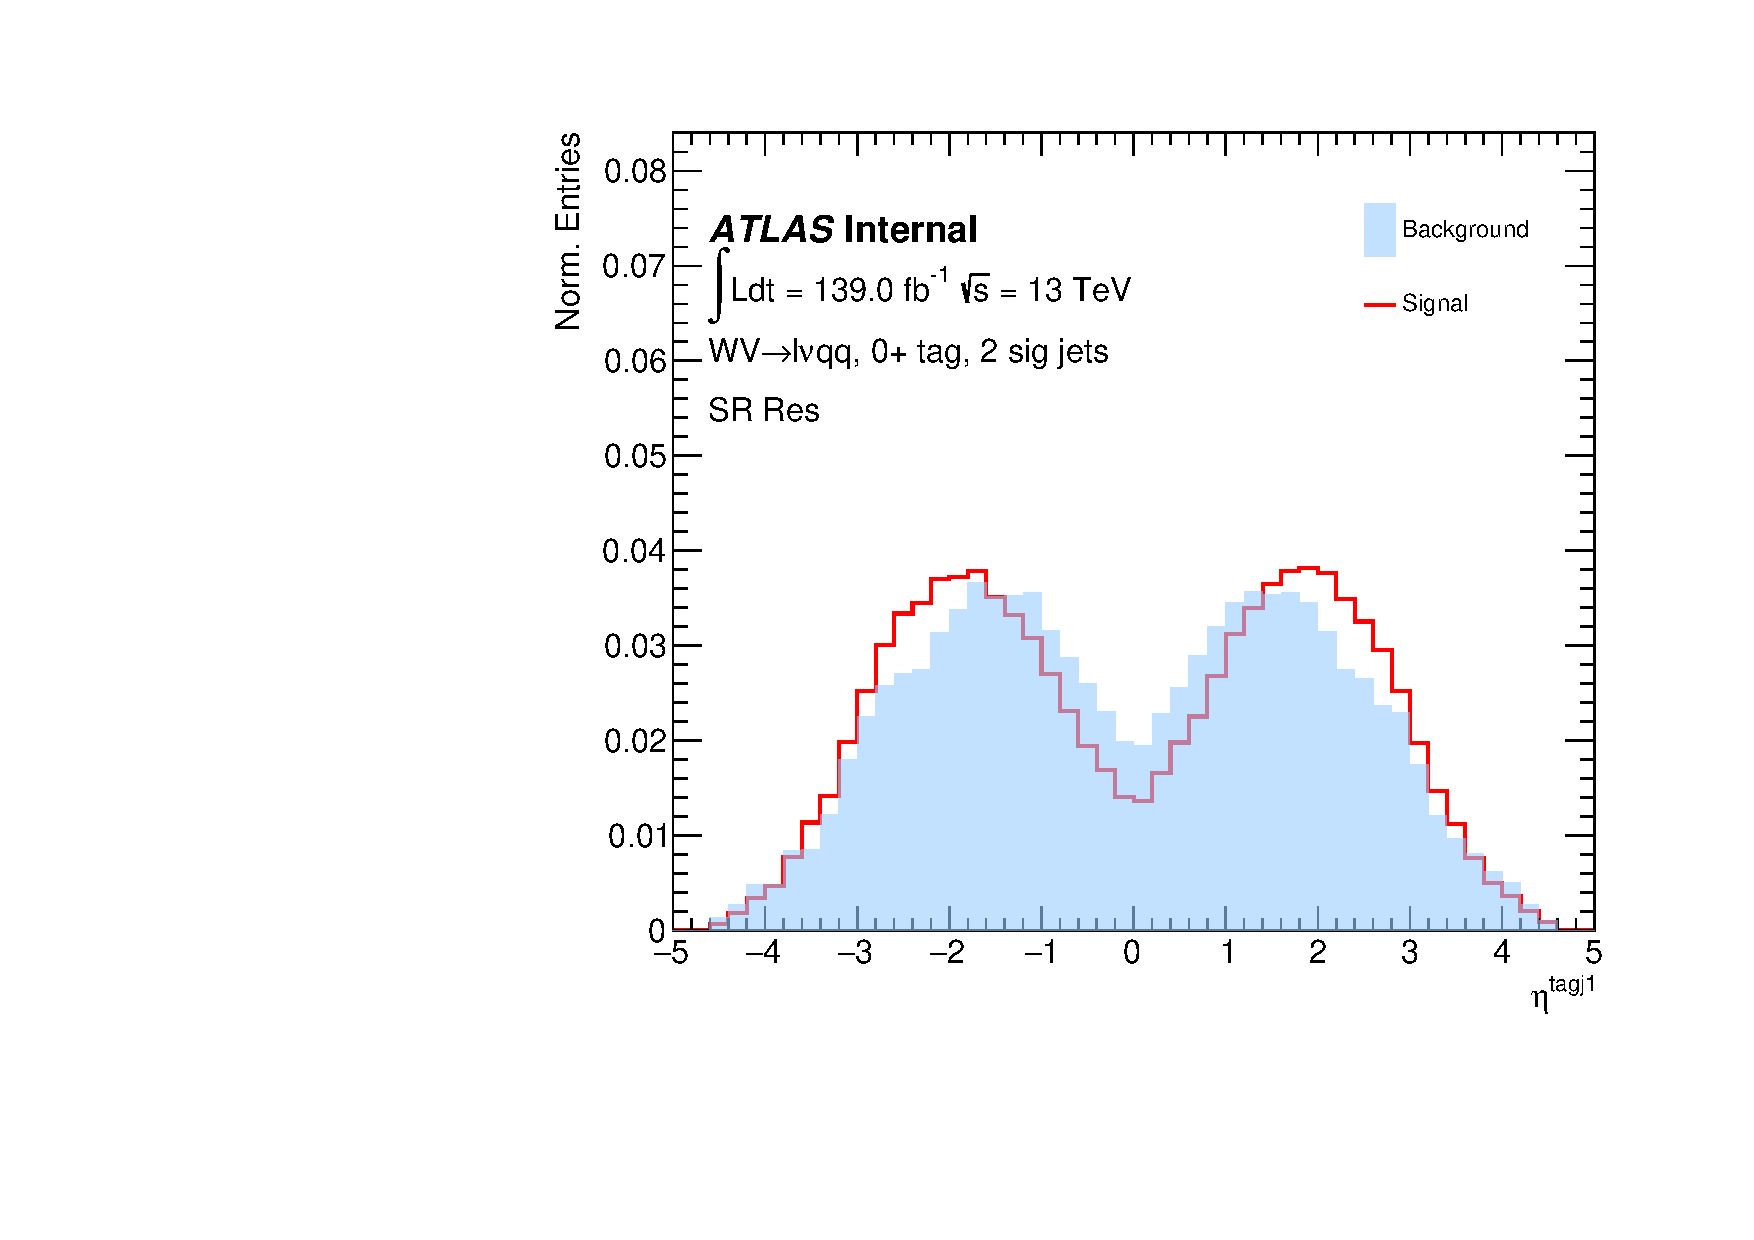
\includegraphics[width=0.3\textwidth]{figures/ml_dnn/variables/SR_Res/norm_plot_resolved_tagJ1_eta.pdf}}\quad
  \subfloat[]{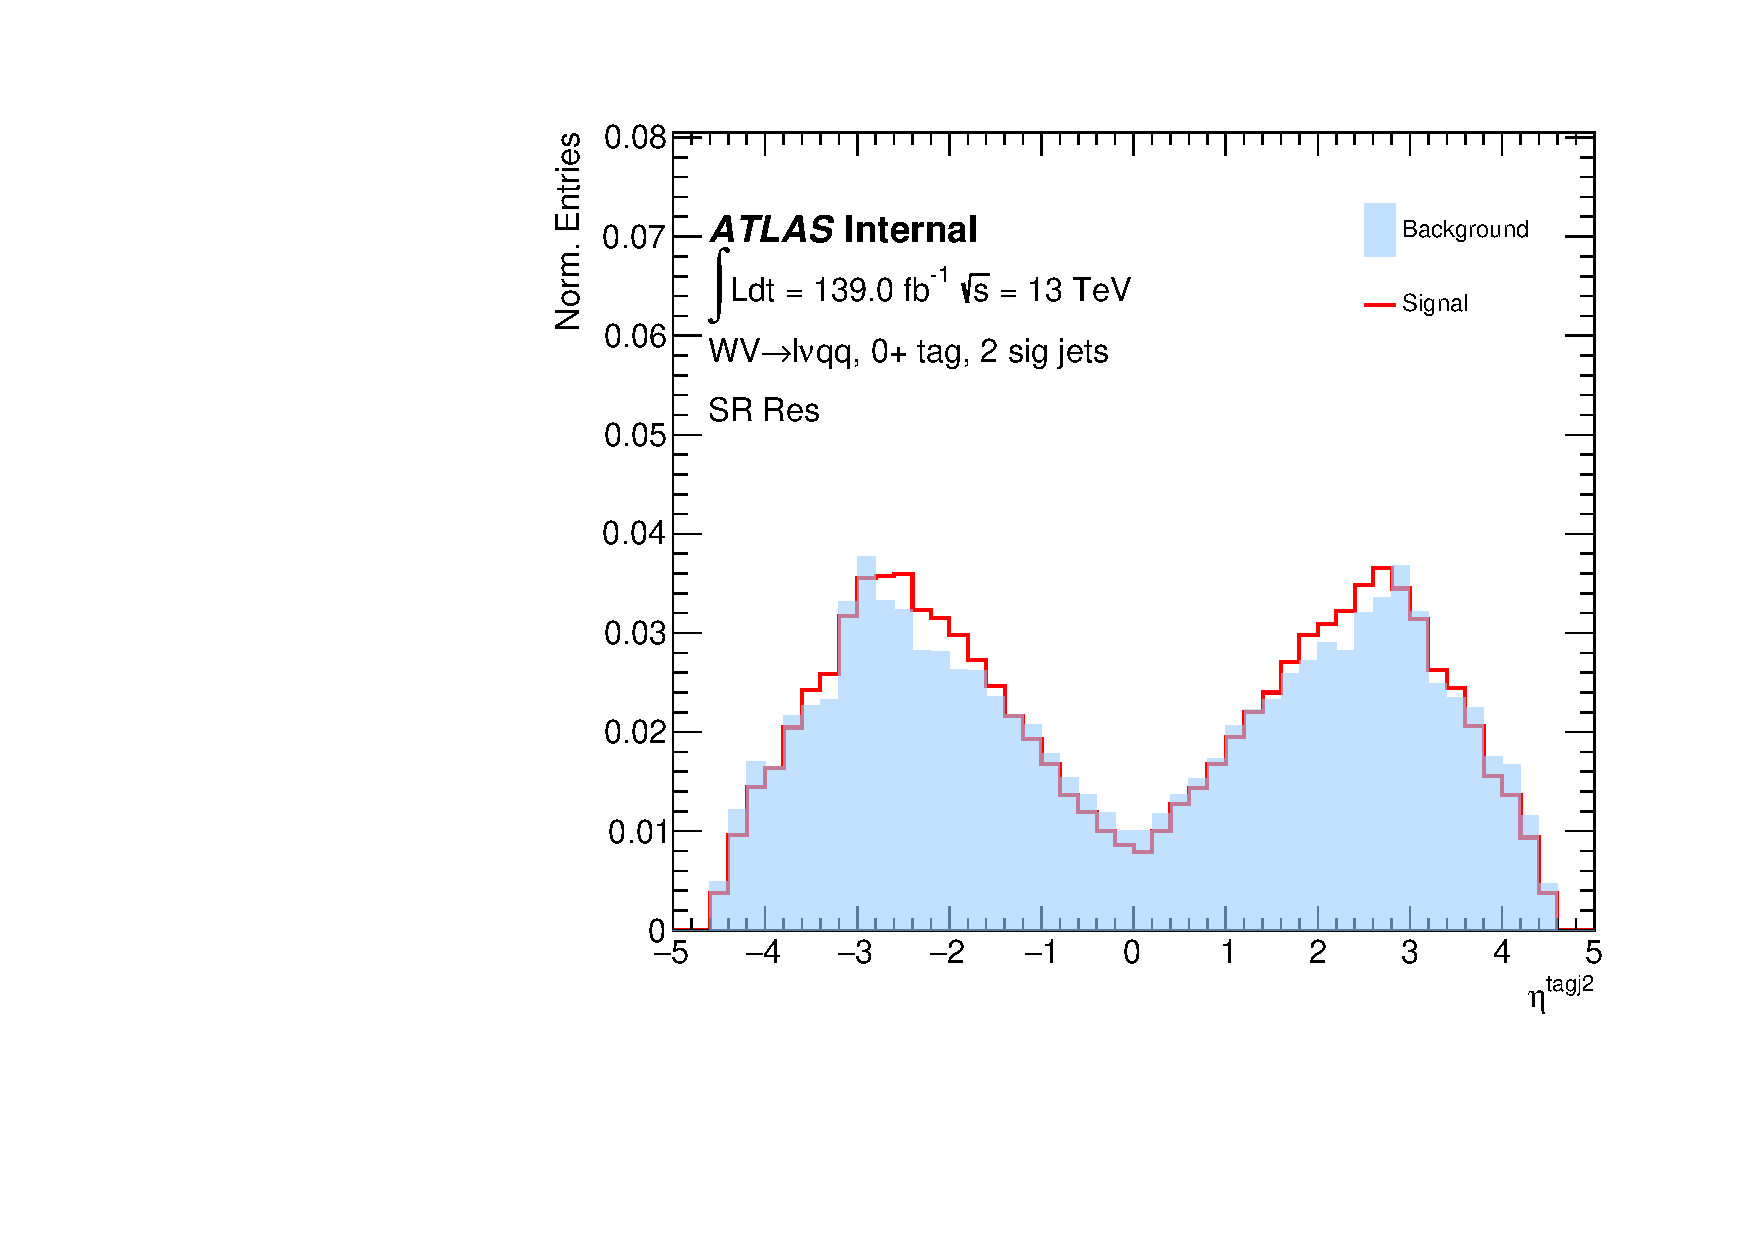
\includegraphics[width=0.3\textwidth]{figures/ml_dnn/variables/SR_Res/norm_plot_resolved_tagJ2_eta.pdf}}
  
  % Row 5
  \subfloat[]{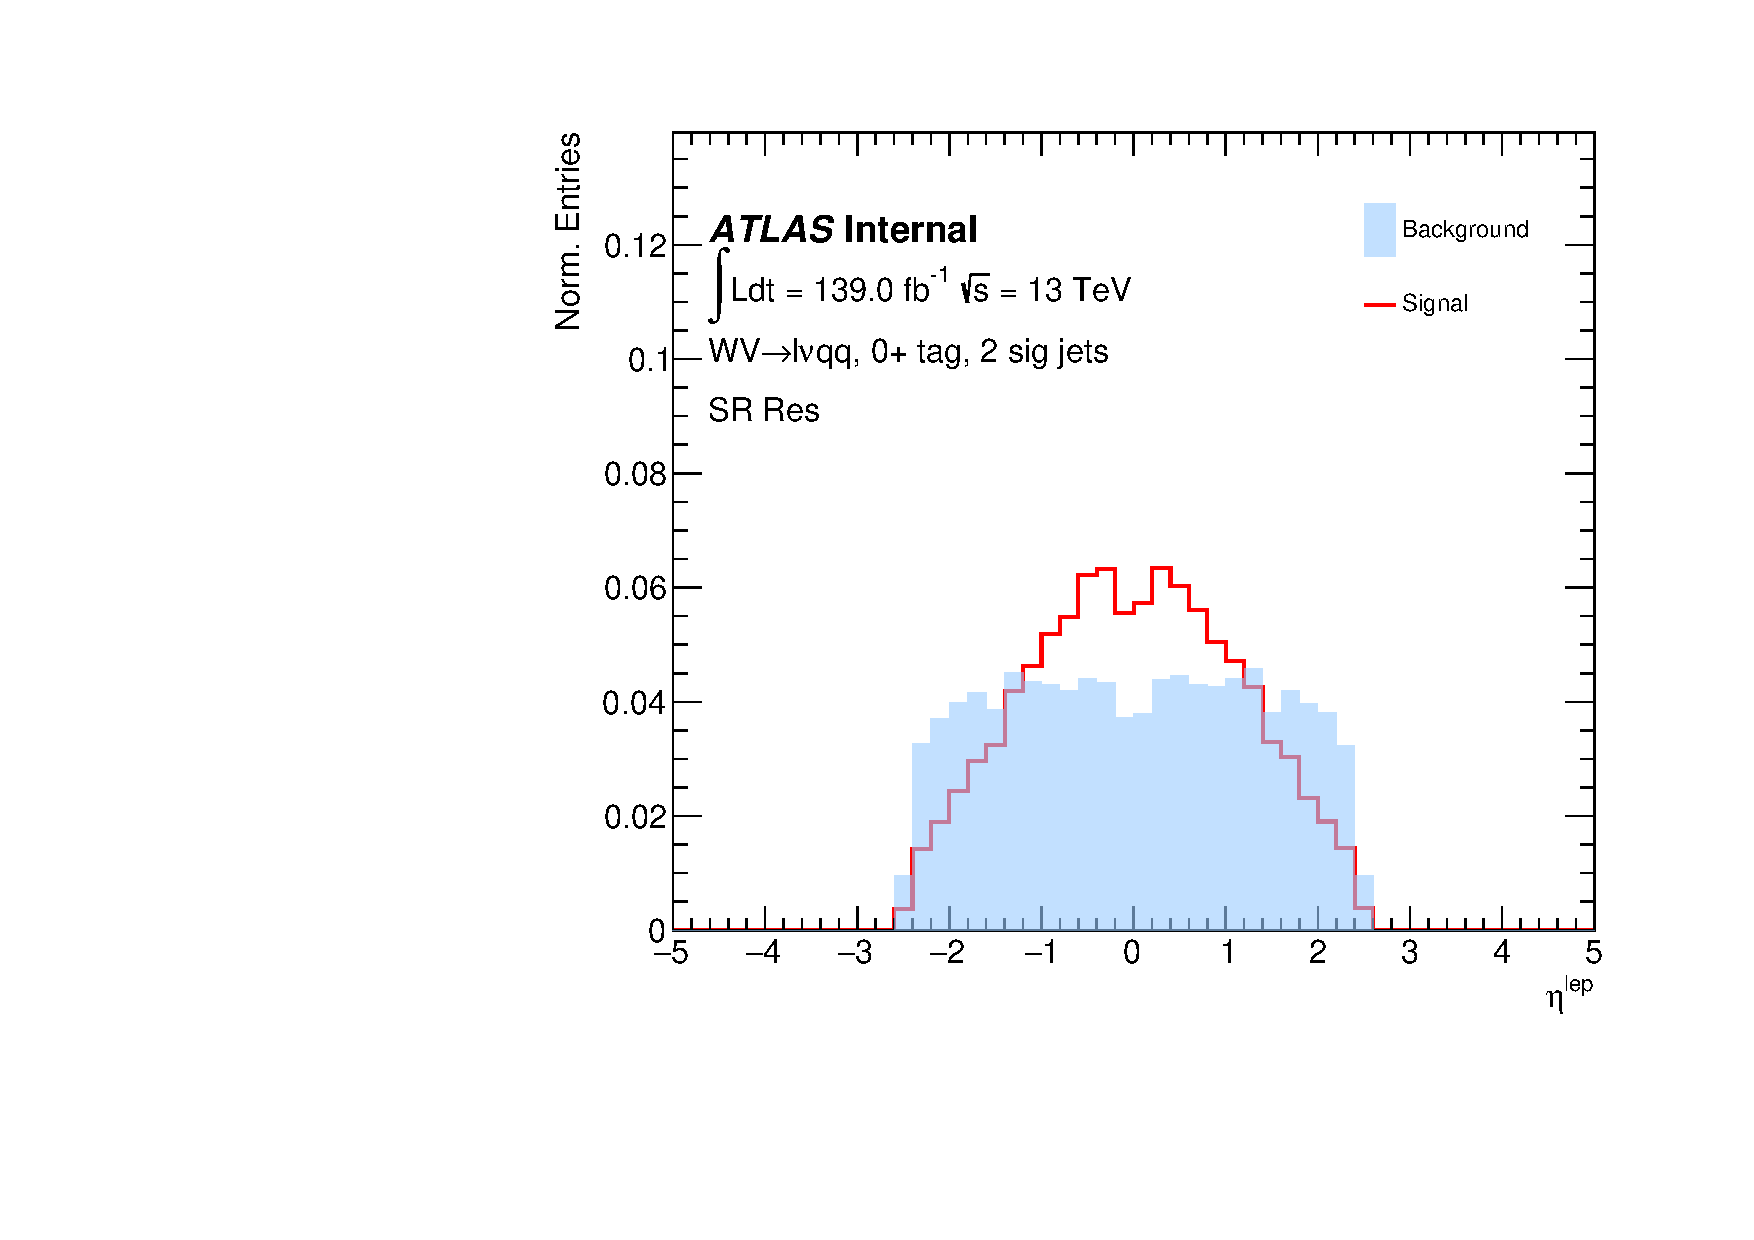
\includegraphics[width=0.3\textwidth]{figures/ml_dnn/variables/SR_Res/norm_plot_lep_eta.pdf}}\quad
  \subfloat[]{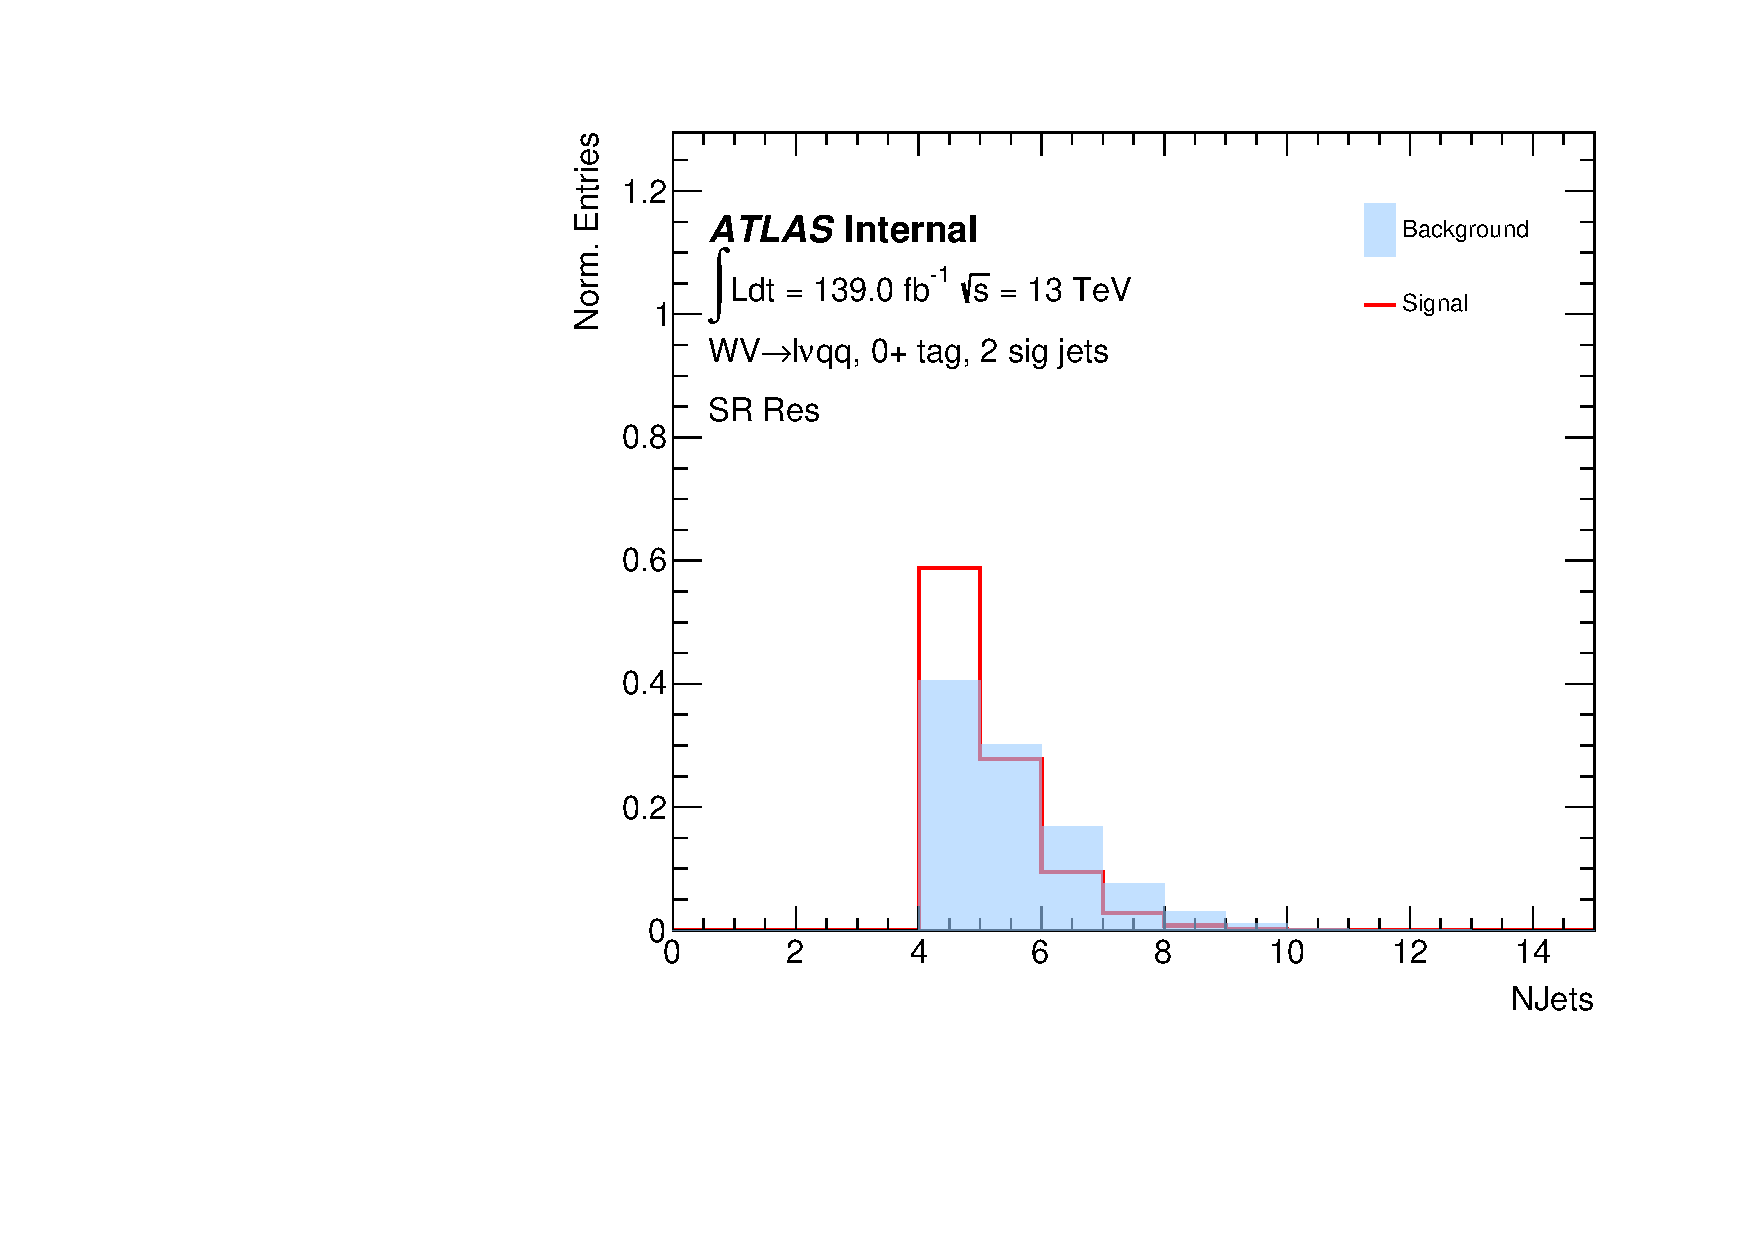
\includegraphics[width=0.3\textwidth]{figures/ml_dnn/variables/SR_Res/norm_plot_NJets.pdf}}\quad
  \subfloat[]{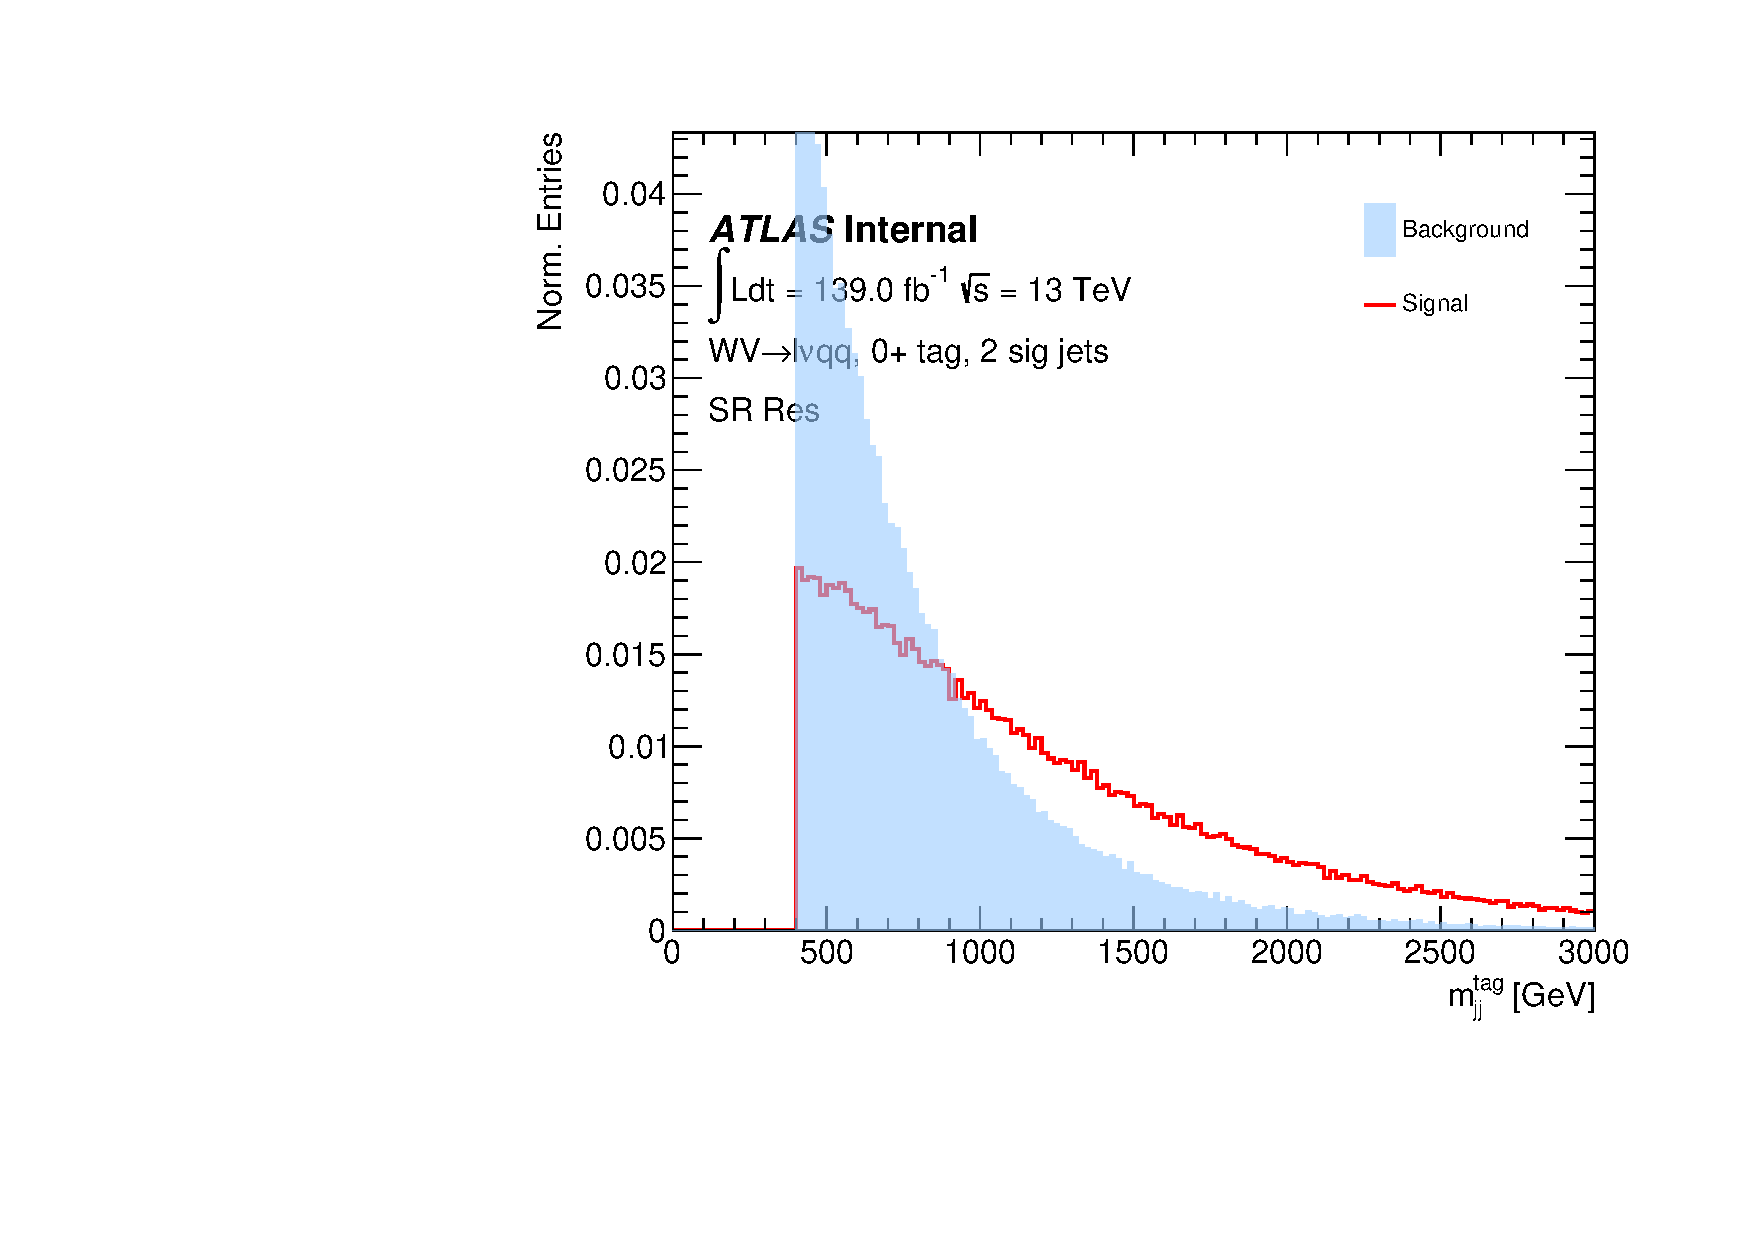
\includegraphics[width=0.3\textwidth]{figures/ml_dnn/variables/SR_Res/norm_plot_resolved_tagMjj.pdf}}
  
  % Row 6
  \subfloat[]{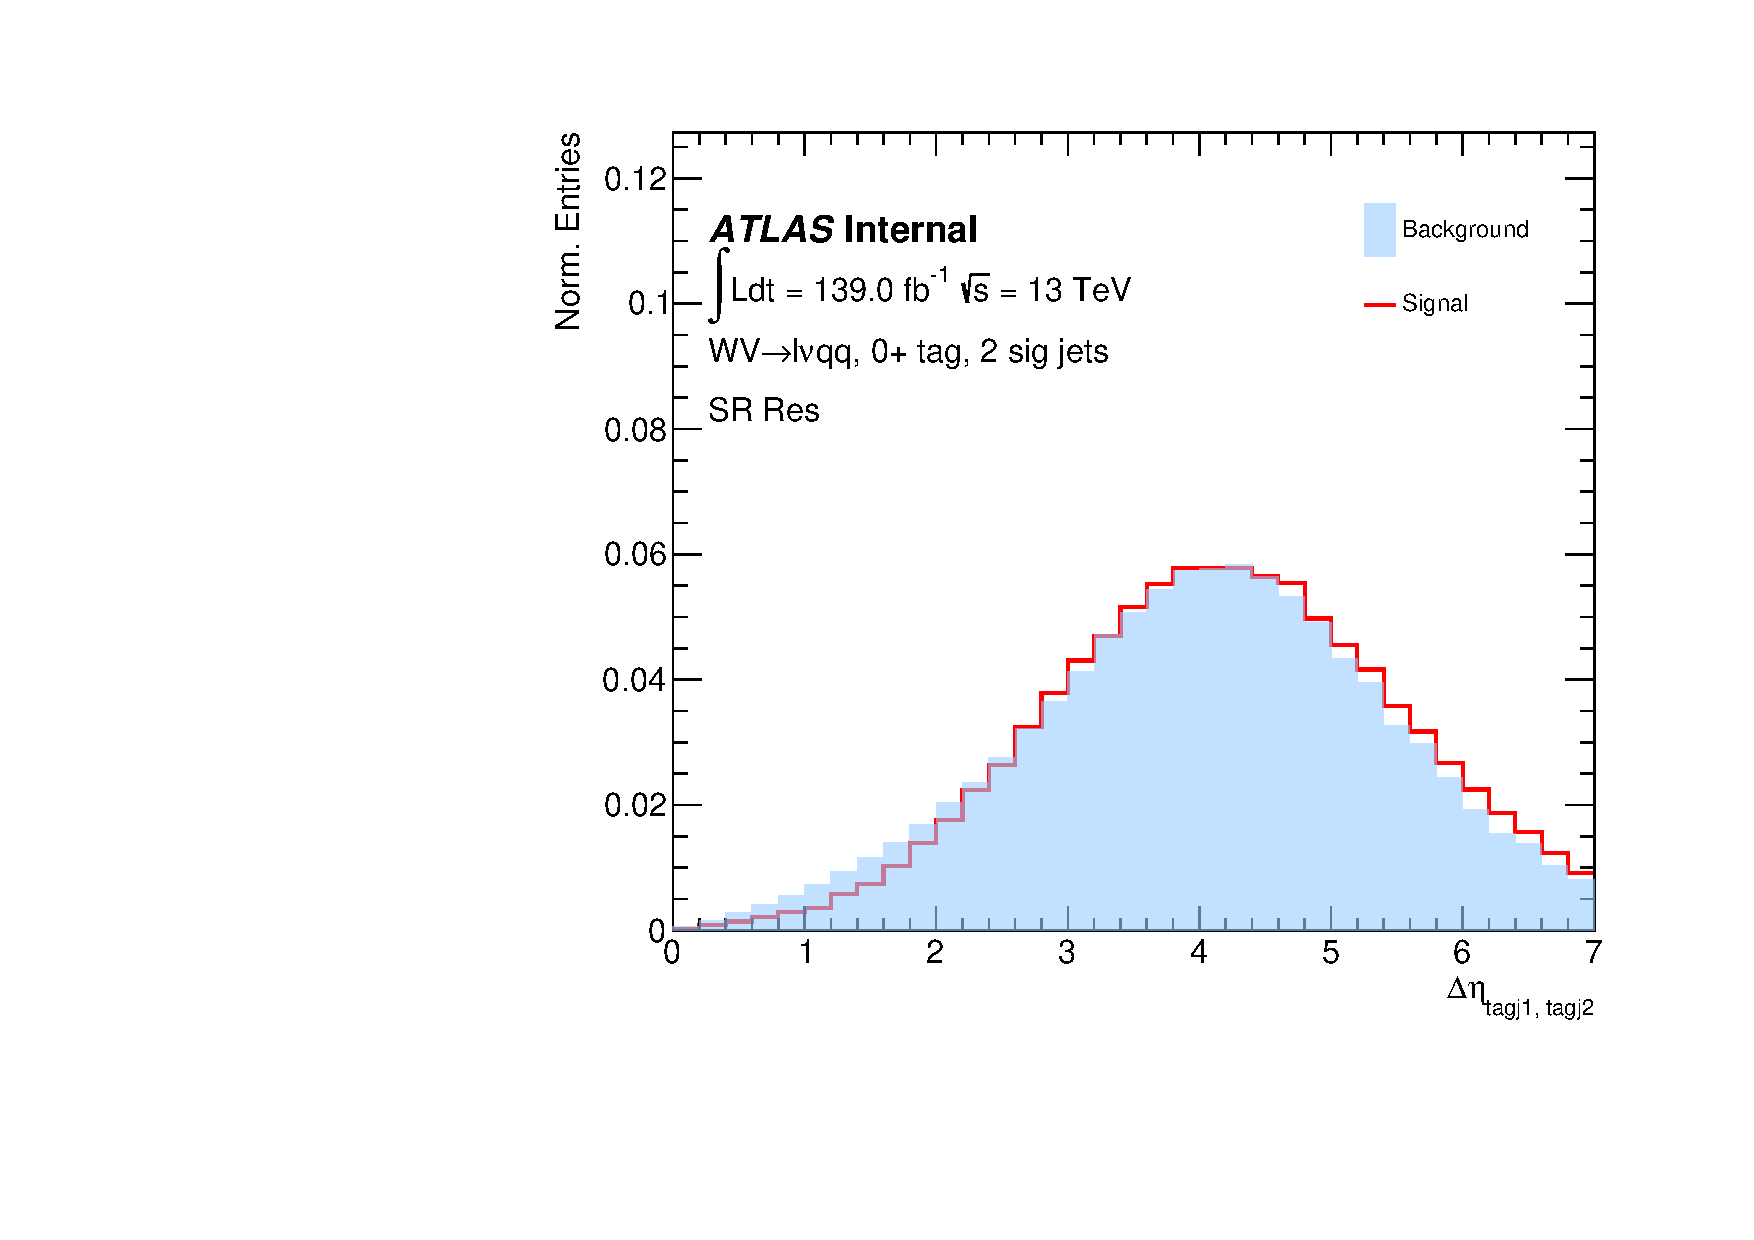
\includegraphics[width=0.3\textwidth]{figures/ml_dnn/variables/SR_Res/norm_plot_resolved_tagJdEta.pdf}}\quad
  \subfloat[]{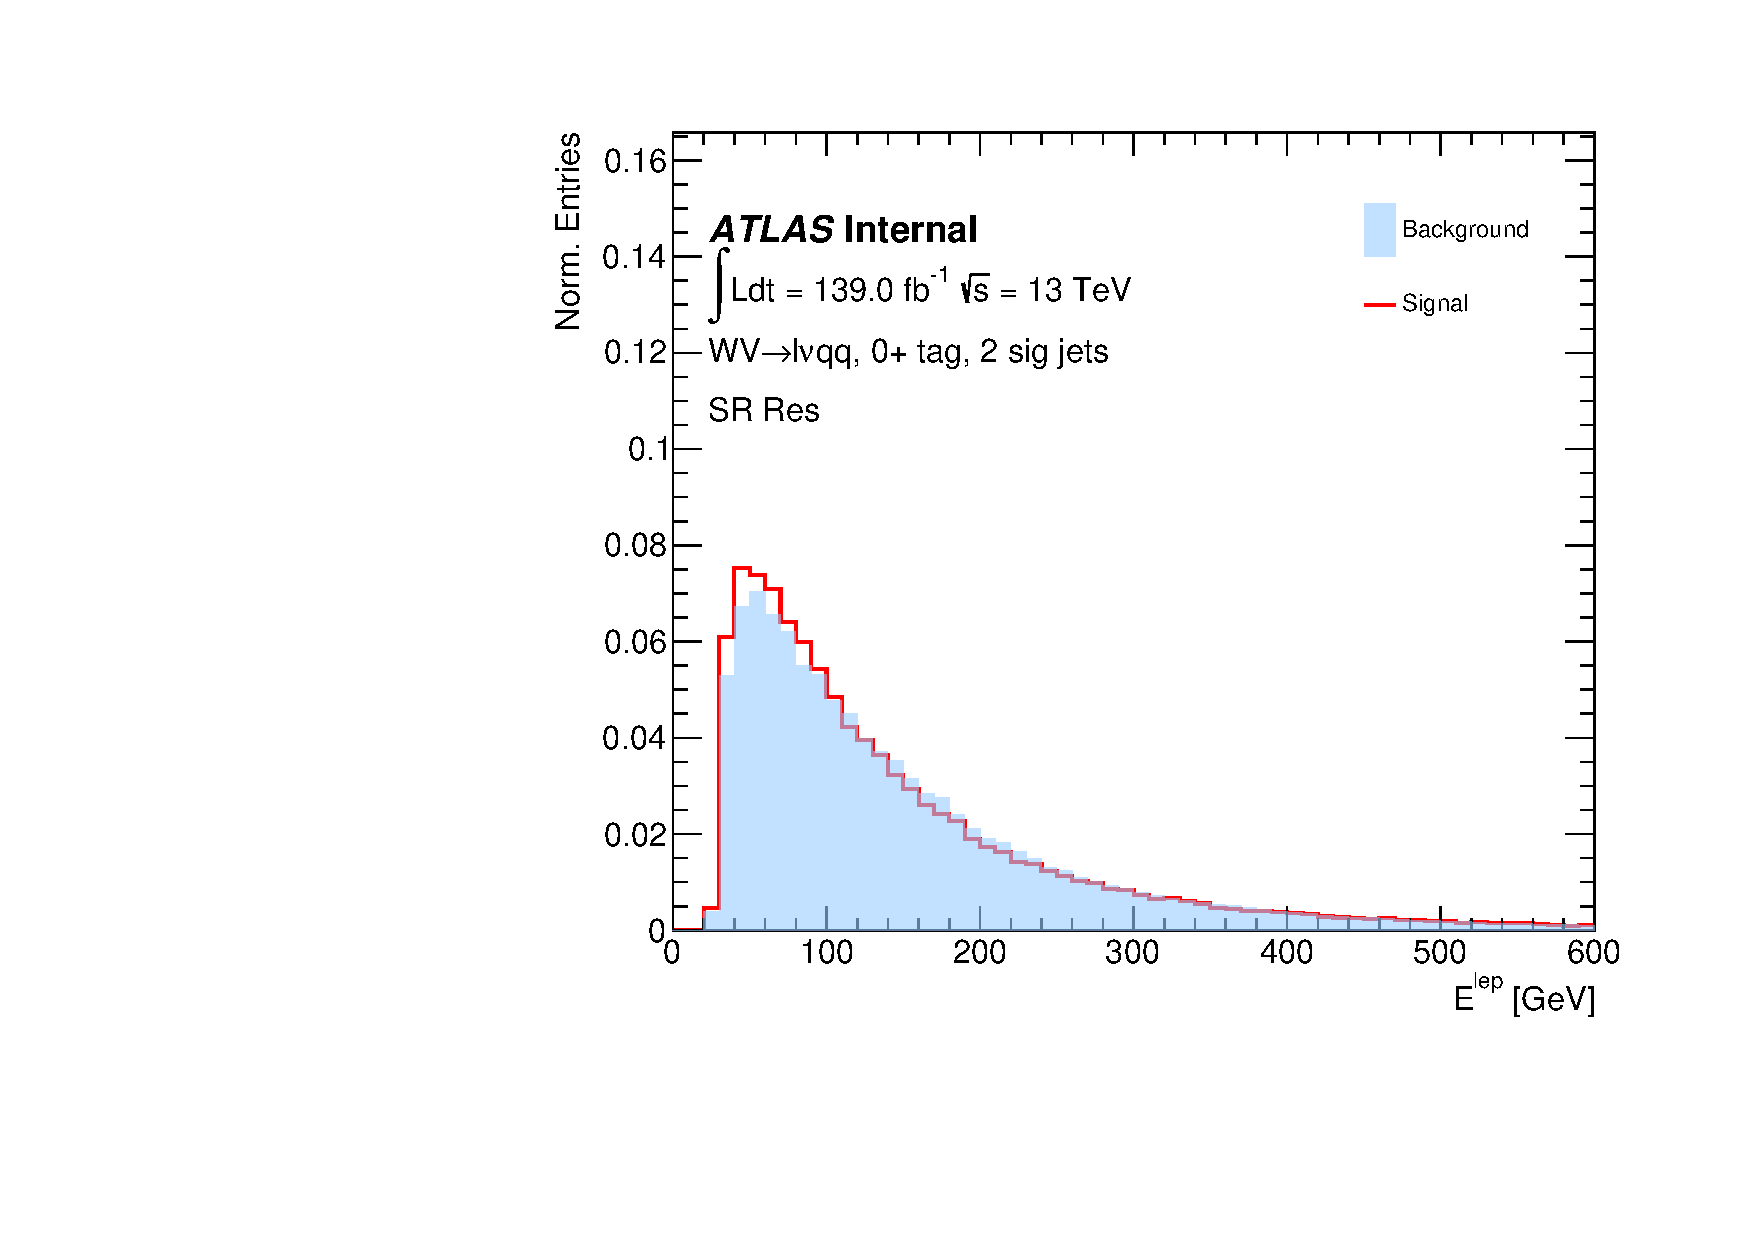
\includegraphics[width=0.3\textwidth]{figures/ml_dnn/variables/SR_Res/norm_plot_lep_e.pdf}}
  
  \caption{Distributions of input variables in the Resolved SR (Continued)}
  \label{fig:res_inputs-part2}
\end{figure}



%%%\clearpage
%%%\section{Trainings and Validations}
%%%\label{trainings_and_validations}
%%%
%%%Figure~\ref{fig:ROCChecks} presents a comparison of the performance between the initial and final DNN models within both the merged and resolved categories, with the results indicating similar levels of effectiveness.
%%%Within this context, signal efficiency and background rejection (rates) are defined as follows:
%%%
%%%\begin{equation}
%%%  Signal \ Efficiency = \frac{\# \ of \ Signal \ events \ with \ DNN > X}{\# \ of \ Signal \ events}
%%%\end{equation}
%%%\begin{equation}
%%%  Background \ Rejection = \frac{\# \ of \ Background \ events \ with \ DNN < X}{\# \ of \ Background \ events}.
%%%\end{equation}
%%%
%%%
%%%\begin{figure}[ht]
%%%      \centering
%%%       \subfloat[\emph{ROC Curve}]{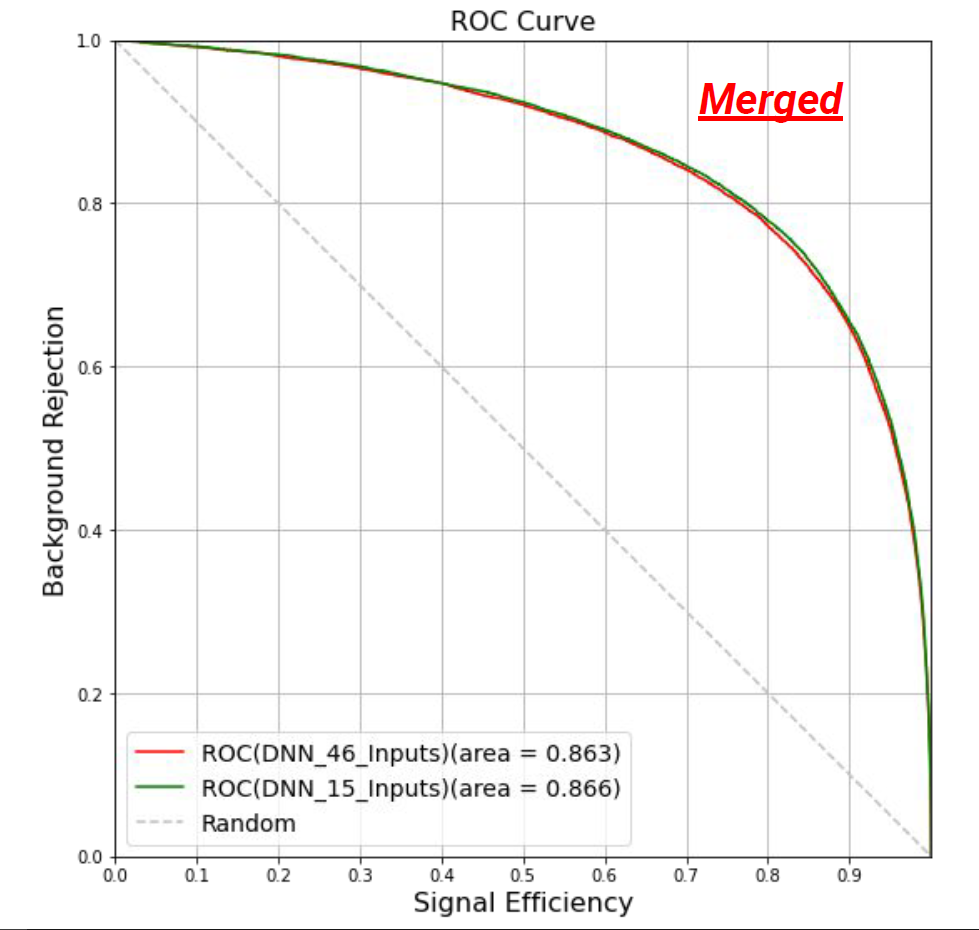
\includegraphics[width=0.4\textwidth]{figures/ml_dnn/ROCImpactMerged.png}}
%%%       \subfloat[\emph{ROC Curve}]{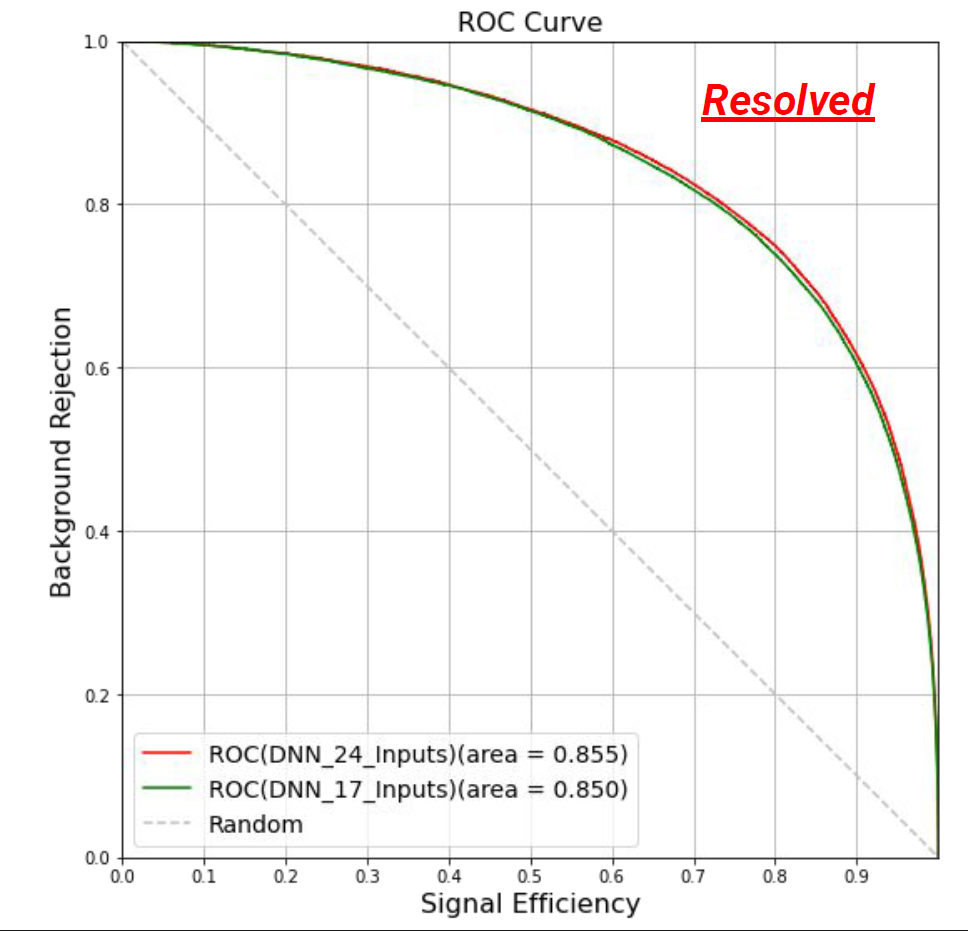
\includegraphics[width=0.4\textwidth]{figures/ml_dnn/ROCImpactRes.png}}
%%%       \caption{ROC curves for the DNN models in the merged (a) and resolved (b) categories. Here, "area" refers to the AUC (Area Under the ROC Curve). The AUC values are computed to offer quantitative measures of performance.}
%%%       \label{fig:ROCChecks}
%%%\end{figure}

\clearpage
\section{Trainings and Validations}
\label{trainings_and_validations}

%Distinct models are trained for the merged and resolved regimes. In the merged regime, a unified model is trained using samples from both the high purity and low purity signal regions. A dedicated model is utilized for the resolved signal region. For each regime, the MC sample is bifurcated by event number: half is allocated for DNN training, and the remainder for validation. Signal EW $VV+jj$ events are categorized as "1" and background events as "0".

%Binary cross-entropy is selected as the loss function, as illustrated in Figure \ref{fig:LossAndAccuracy}. Trials with both the Adam and SGD (stochastic gradient descent) optimizers on the DNN models suggest that SGD is preferable due to its role in refining the distribution of DNN scores.

We train separate models for the merged and resolved categories. In the merged category, a single model is trained with events from both high and low purity signal regions, while the resolved category uses its own dedicated model. For each category, we split the MC sample into two: one part for training the DNN and the other for validation. Signal EW $VV+jj$ events are labeled as ``1'' and background events as ``0''.

The loss function used is binary cross-entropy, as shown in Figure \ref{fig:LossAndAccuracy}. Experiments with Adaptive Moment Estimation (Adam) and Stochastic Gradient Descent (SGD) optimizers reveal that SGD is preferred for its effectiveness in adjusting the distribution of DNN scores.

%%%k-fold
In this analysis, we employ the k-fold cross-validation method to fully leverage our MC samples, ensuring an unbiased evaluation of performance. 
We utilize a 5-fold cross-validation strategy. This approach divides the dataset into 5 equally sized parts(or folds), then the DNN is trained and validated 5 times. 
During each of the five iterations, four folds are used for training the model, while the remaining fold serves as the validation set. 
This cyclical process ensures that every MC event in the SRs is used for both training and validation across the iterations.
Figure \ref{fig:kfoldValidations} provides a clear indication of the DNN approach's reliability across different subsets of the dataset.

For practicality and reliability, I employs a 2-fold cross-validation method for the DNN approach. The complete MC sample is evenly divided into training and testing datasets. The consistent performance between these datasets, highlighted in Figure \ref{fig:ROCValidations}, indicates no training set bias. 


Figure~\ref{fig:1lepDNN_performance} demonstrates the effective separation between signal and background in the DNN distribution for both merged and resolved regimes. Figure~\ref{fig:1lepDNNoutputs} presents the DNN score distributions across all three signal regions, featuring partially blinded data bins.
%Additionally, Figure \ref{fig:1lepDNNoutputs} displays the DNN scores across all three signal regions.


\begin{figure}[ht]
      \centering
       \subfloat[\emph{Loss curve}]{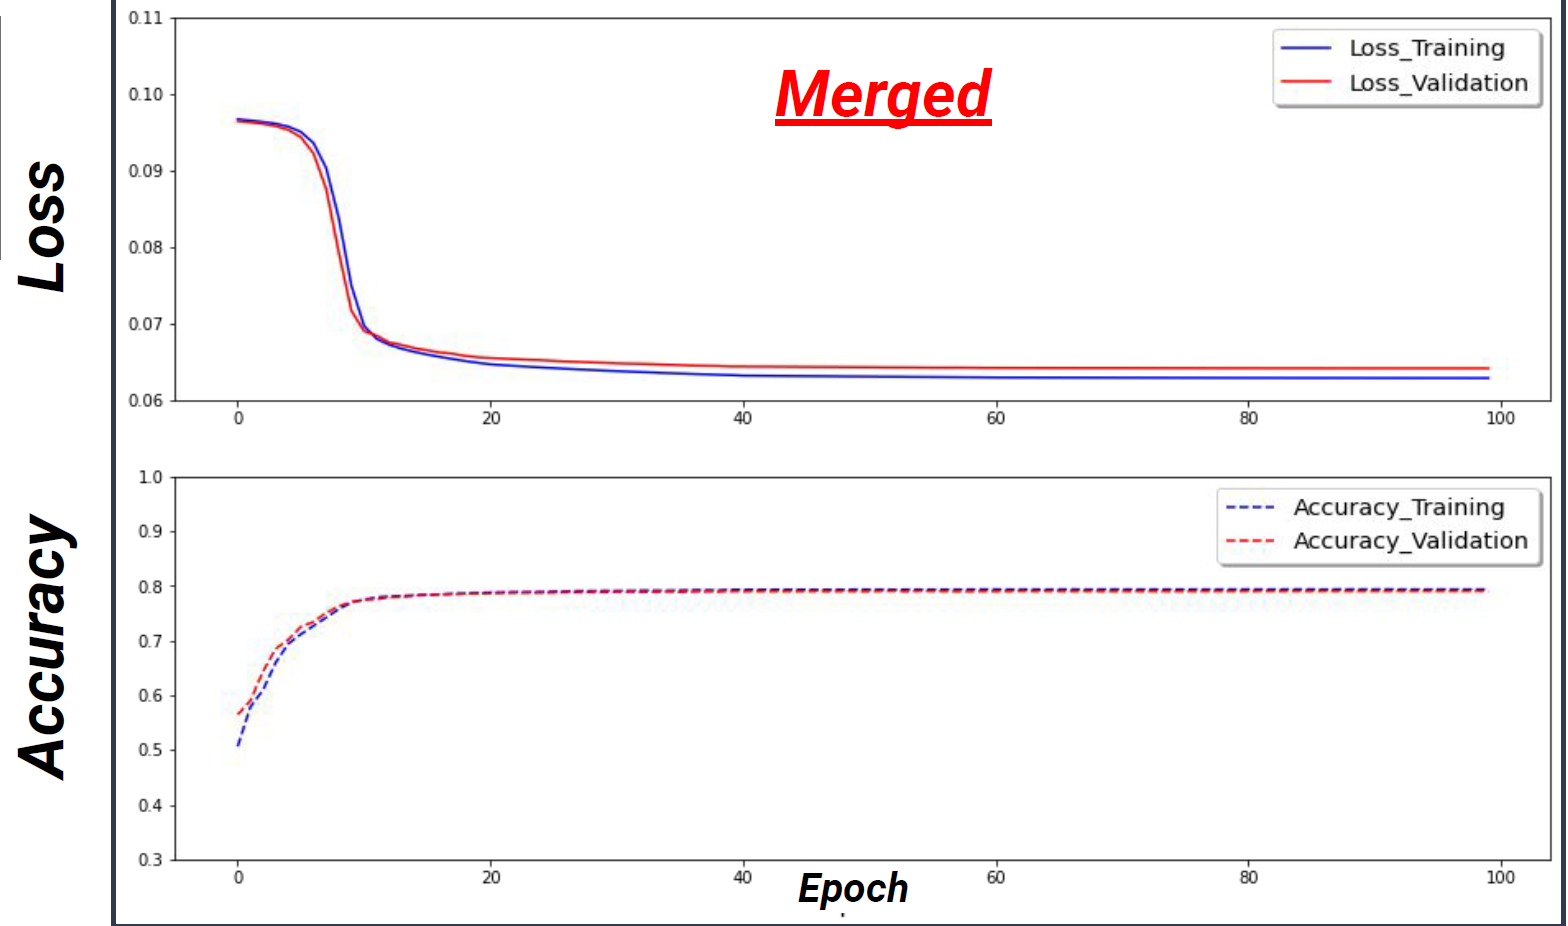
\includegraphics[width=0.45\textwidth]{figures/ml_dnn/loss_mer.png}}
       \subfloat[\emph{Loss curve}]{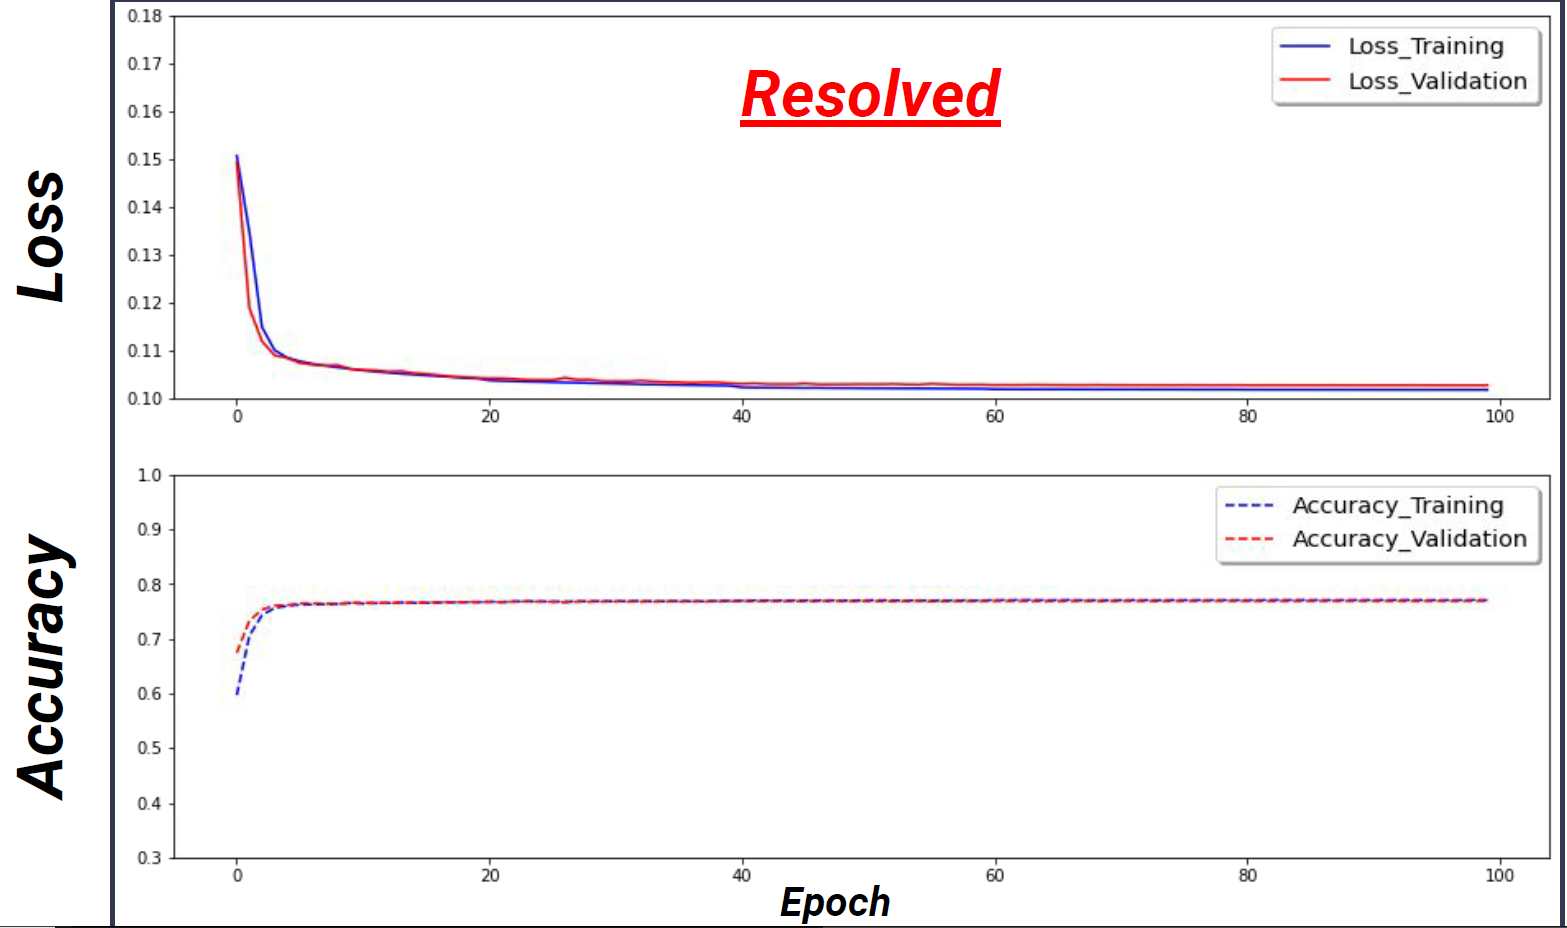
\includegraphics[width=0.45\textwidth]{figures/ml_dnn/loss_res.png}}
       \caption{Trainings for the DNN models in the merged and resolved regimes.}
       \label{fig:LossAndAccuracy}
\end{figure}

\begin{figure}[ht]
      \centering
       \subfloat[\emph{ROC curve}]{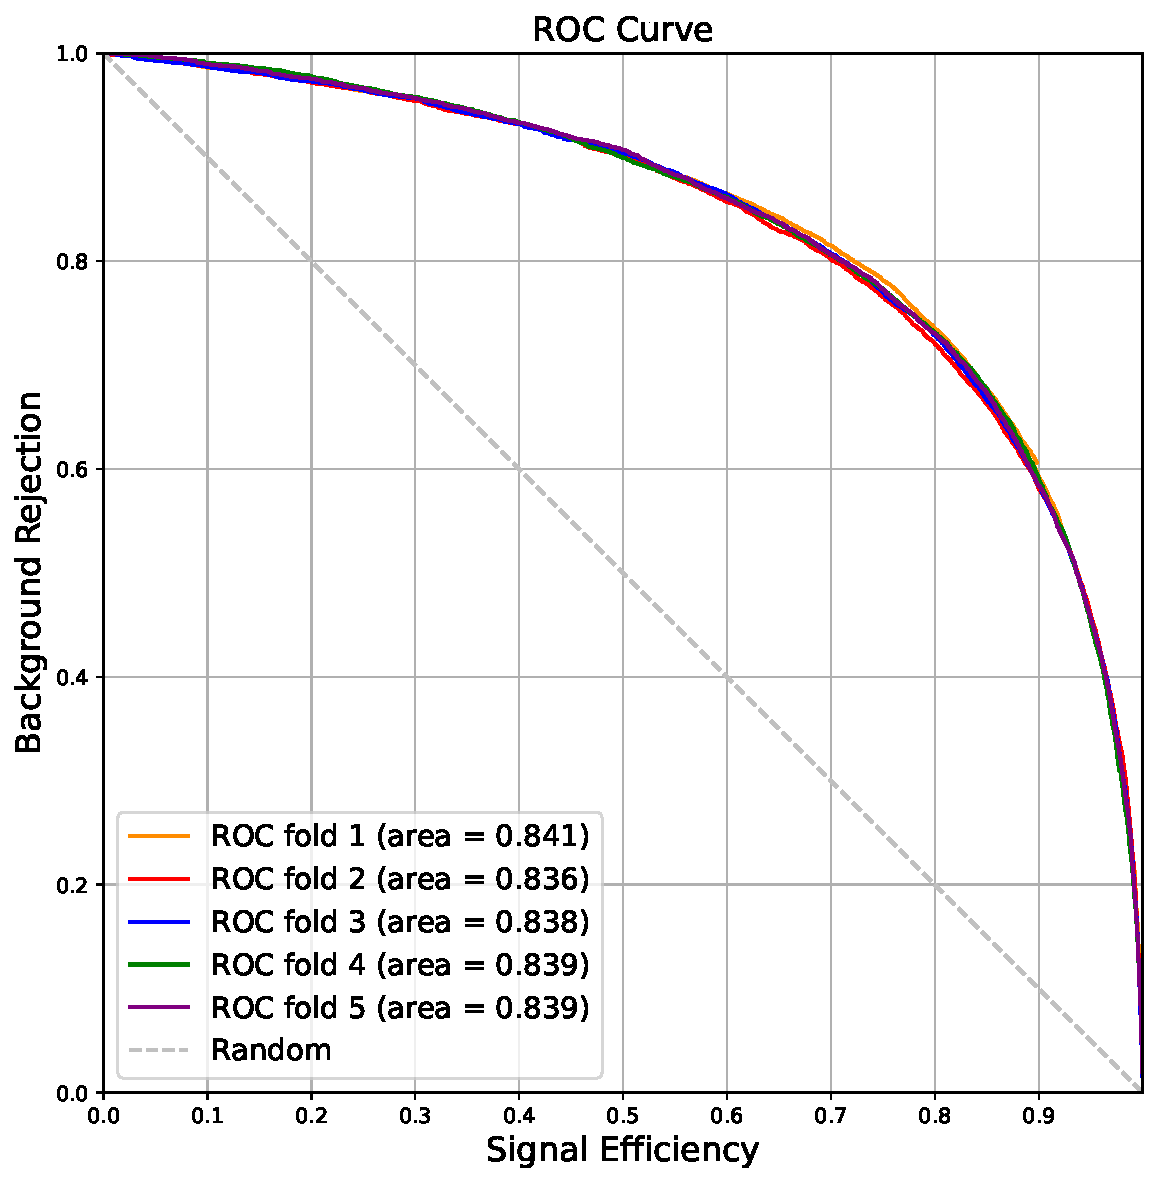
\includegraphics[width=0.45\textwidth]{figures/ml_dnn/kfold/roc_curve_mer.pdf}}
       \subfloat[\emph{ROC curve}]{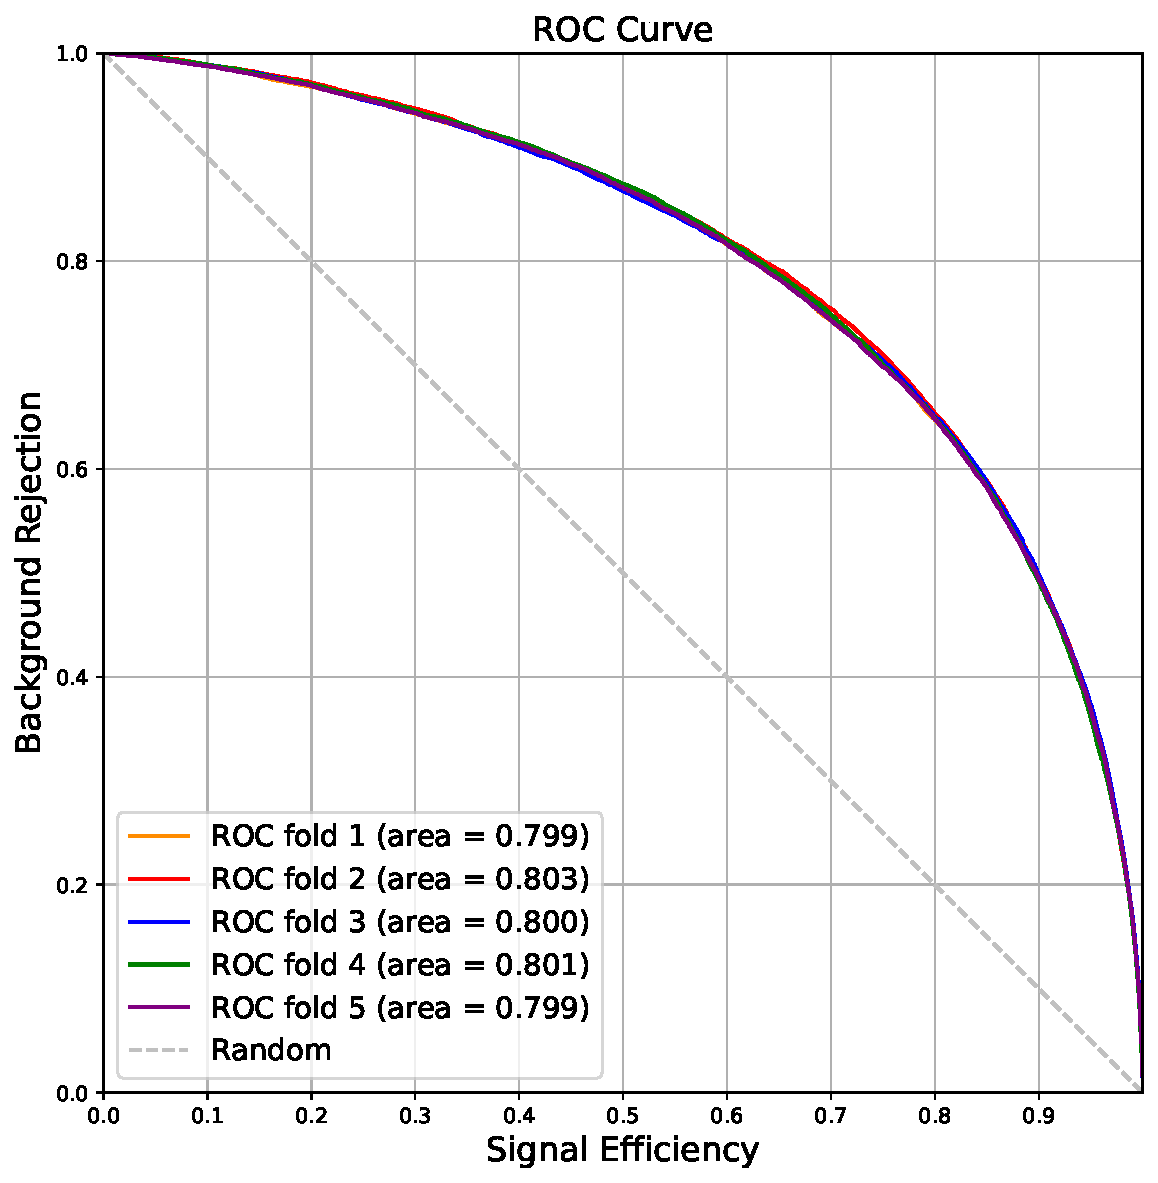
\includegraphics[width=0.45\textwidth]{figures/ml_dnn/kfold/roc_curve_res.pdf}}
       \caption{K-fold cross-validation for the DNN model trained in the merged and resolved regimes.}
       \label{fig:kfoldValidations}
\end{figure}


\begin{figure}[ht]
      \centering
       \subfloat[\emph{ROC curve}]{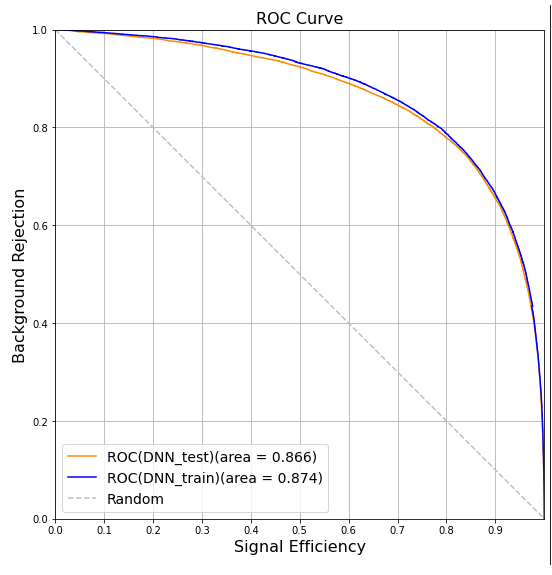
\includegraphics[width=0.45\textwidth]{figures/ml_dnn/roc_mer.png}}
       \subfloat[\emph{ROC curve}]{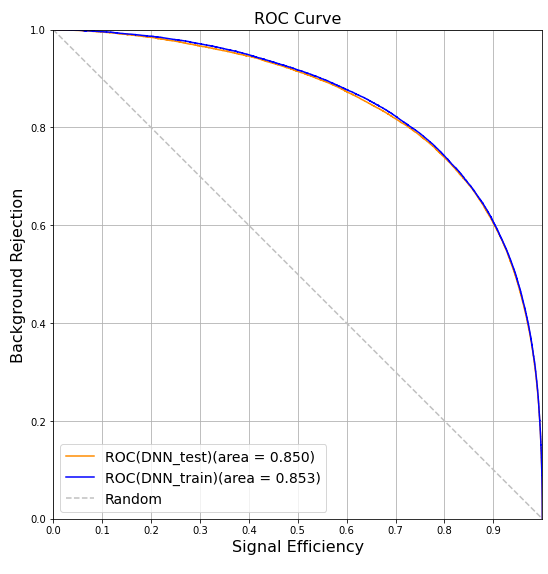
\includegraphics[width=0.45\textwidth]{figures/ml_dnn/roc_res.png}}
       \caption{Validation for the DNN model trained in the merged and resolved regimes.}
       \label{fig:ROCValidations}
\end{figure}

\begin{figure}[ht]
      \centering
       \subfloat[\emph{DNN Merged}]{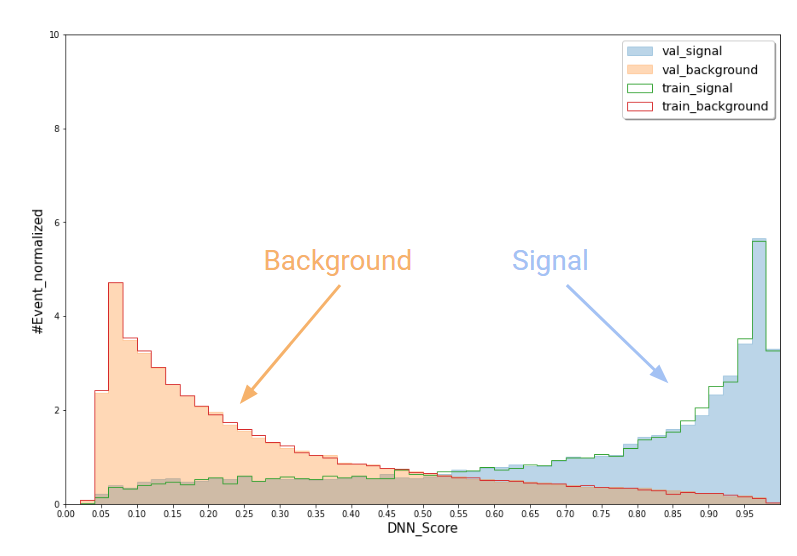
\includegraphics[width=0.45\textwidth]{figures/ml_dnn/dnn_dist/dnn_norm_mer.PNG}}
       \subfloat[\emph{DNN Resolved}]{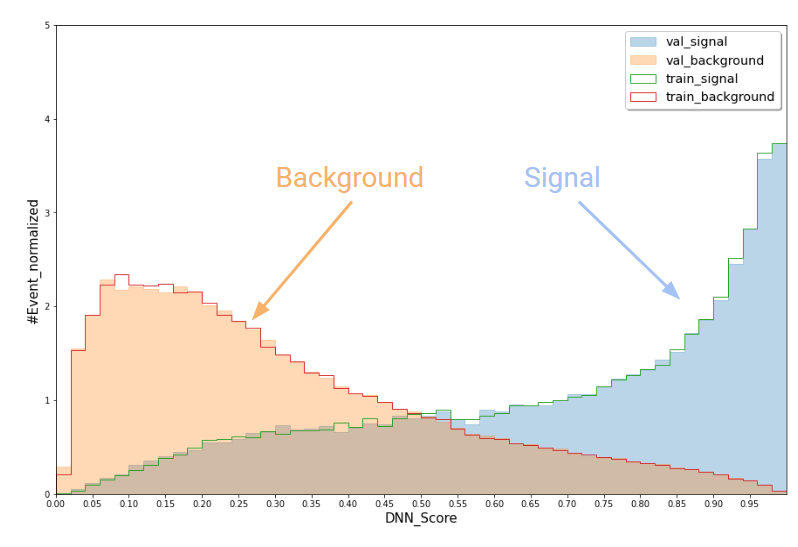
\includegraphics[width=0.45\textwidth]{figures/ml_dnn/dnn_dist/dnn_norm_res.PNG}}
       \caption{Performance for the DNN model trained in the merged and resolved regimes.}
       \label{fig:1lepDNN_performance}
\end{figure}

\begin{figure}[ht]
 \begin{center}
  \subfloat[DNN HP]{\includegraphics[width=0.3\textwidth]{figures/ml_dnn/Region_distDNN_DSRVBSHP_BMin0_J0_incJet1_L1_T0_incFat1_Y6051_incTag1_Fat1_Prefit.pdf}}
  \subfloat[DNN LP]{\includegraphics[width=0.3\textwidth]{figures/ml_dnn/Region_distDNN_DSRVBSLP_BMin0_J0_incJet1_L1_T0_incFat1_Y6051_incTag1_Fat1_Prefit.pdf}}
  \subfloat[DNN Res]{\includegraphics[width=0.3\textwidth]{figures/ml_dnn/Region_distDNN_DSRVBSTight_BMin0_T0_Y6051_incTag1_J2_L1_incJet1_Prefit.pdf}}
  \caption{DNN score distributions for the high purity merged, low purity merged, and resolved signal regions.}
 \label{fig:1lepDNNoutputs}
 \end{center}
\end{figure}

%%%\clearpage
%%%\subsection{Fit results in unblinded SR}

